\documentclass[journal, letterpaper]{IEEEtran}
\usepackage{graphicx}
\usepackage{url}        
\usepackage{amsmath}
\usepackage{longdivision}
\usepackage{amssymb}  
\usepackage{textgreek}	% Greek to me, dawg
\usepackage{listings}
\usepackage{csvsimple}
\usepackage{longtable}
\usepackage{cmbright}
\usepackage[most]{tcolorbox}
\newtcolorbox{mybox}[2][]{breakable,sharp corners, skin=enhancedmiddle jigsaw,parbox=false,
boxrule=0mm,leftrule=2mm,boxsep=0mm,arc=0mm,outer arc=0mm,attach title to upper,
after title={.\ }, coltitle=black,colback=blue!10,colframe=black, title={#2},
fonttitle=\bfseries,#1}

\newtcolorbox{myboxg}[2][]{breakable,sharp corners, skin=enhancedmiddle jigsaw,parbox=false,
boxrule=0mm,leftrule=2mm,boxsep=0mm,arc=0mm,outer arc=0mm,attach title to upper,
after title={.\ }, coltitle=black,colback=gray!10,colframe=black, title={#2},
fonttitle=\bfseries,#1}

\newtcolorbox{myboxr}[2][]{breakable,sharp corners, skin=enhancedmiddle jigsaw,parbox=false,
boxrule=0mm,leftrule=2mm,boxsep=0mm,arc=0mm,outer arc=0mm,attach title to upper,
after title={.\ }, coltitle=black,colback=red!10,colframe=black, title={#2},
fonttitle=\bfseries,#1}

\begin{document}

% Title page
\title{MATH2501: Linear Algebra}
\author{Haeohreum Kim (z5480978)}
\maketitle
\section{Review of first year linear algebra}
\subsection{Linear systems of equations}
\begin{mybox}{Objective} \\ 
    To be able to determine how many solutions a system of 
    linear equations has, and to find al these solutions
    \begin{enumerate}
        \item How many solutions can a system of linear equations have?
        \item What is the most commonly used method of solving linear systems?
        \item How do you use this method to determine the number of solutions in a system?
    \end{enumerate}
\end{mybox}

    \begin{myboxg}{Example} Solve the following linear system$$
    \begin{cases}
        2x_1 - x_2 - 3x_3 &= -3 \\ 
        -x_1 + x_2 + 5x_3 + x_4 &= 4 \\
        5x_1 - x_2 + 3x_3 + 3x_4 &= 0
    \end{cases}$$
    This can be represented in matrix form
    $$ 
    \begin{pmatrix}
        2 & -1 & -3 & 0 & -3 \\
        -1 & 1 & 5 & 1 & 4 \\ 
        5 & -1 & 3 & 3 & 0 
    \end{pmatrix}
    $$
    Using Gaussian Elimination, we can reduce this to
    $$ 
    \begin{pmatrix}
        2 & -1 & -3 & 0 & -3 \\ 
        0 & 1/2 & 7/2 & 1 & 5/2 \\ 
        0 & 0 & 0 & 0 & 0
    \end{pmatrix}
    $$
    \textbf{Since the last column is non-leading, the system has solutions}. There can be infinite many solutions, or 
    a unique solution. Note that there are \textit{two leading columns}, $x_1$ and $x_2$. \\ \\ 
    This means that $x_3$ and $x_4$ are parameters $\in \mathbb{R}$.
    \begin{align*}
    x_2 /2 + 7x_3/2 + x_4 &= 5/2 \\
    2x_1 - x_2 - 3x_3 &= -3 
    \end{align*}
    Rearranging the two equations, we get:
    \begin{align*}
    x_2 &= -7x_3 - 2x_4 + 5 \\
    x_1 &= x_2/2 - 3x_3/2 - 3/2
    \end{align*}
    Now since $x_2$ is not a parameter, we must subsitute $x_2$ into $x_1$:
    $$
    x_1 = 1/2 \cdot (-4x_3 - 2x_4 + 2)
    $$
    We now have the (infinitely many) solutions.
\end{myboxg}
    \newpage
    \begin{myboxr}{Consistent and inconsistent} \\
        We say a system of equations is \textbf{consistent} if there exists at least one solution,
        and \textbf{inconsistent} if there exists no solution.
    \end{myboxr}
    \subsection{Conditions for a solution to exist}
    \begin{mybox}{Objective} \\ 
        Given a matrix $A$, find conditions on $b_1$, $b_2$ such that the system $Ax = b$ has a solution.
    \end{mybox}
    \begin{myboxg}{Finding conditions for a solution with an arbitrary matrix} \\
        Let $$A = \begin{pmatrix}
            1 & -1 & 3 \\ 
            0 & 2 & -1 \\
            2 & 0 & 5 \\
            -2 & -4 & -3
        \end{pmatrix}$$
        Find conditions for $b_1, b_2, b_3$ and $b_4$ such that $Ax = b$ has a solution. \\ \\
        We must first row reduce on the augmented matrix, 
        in which we find that
        $$ 
        \begin{pmatrix}
            1 & -1 & 3 & b_1 \\ 
            0 & 2 & -1 & b_2 \\
            0 & 0 & 0 & b_3 - 2b_1 - b_2 \\ 
            0 & 0 & 0 & b_4 + 2b_1 + 3b_2
        \end{pmatrix}
        $$
        We can see that the two last rows must be zero for the 
        system of equations to have a solution. Thereby:
        \begin{align*}
            b_3 - 2b_1 - b_2 &= 0 \\
            b_4 + 2b_1 + 3b_2 &= 0
        \end{align*}
        For the system of equations to have solutions.
    \end{myboxg}
    \begin{myboxg}{Finding a unique solution with parameters} \\ 
        Find (for any $c$) the solutions of the system
        \begin{align*}
            x_1 - x_2 &= 3 \\
            x_1 - cx_3 &= 1 \\ 
            -2x_1 + (c-2)x_2 - 4x_3 &= -c-8 
        \end{align*}
        Reducing this, we get
        \begin{align*}
            \begin{pmatrix}
                1 & -1 & 0 & 3 \\
                0 & 1 & -c & -2 \\ 
                0 & 0 & c^2 - 4 & c - 2 
            \end{pmatrix}
        \end{align*}
        Now consider when $c^2 - 4 = 0$.
        \begin{enumerate}
            \item If $c = 2$, then there exists infinite solutions on parameter $x_3$.
            \item If $c = -2$, there exists no solutions (as the last column is leading).
            \item If $c^2 - 4 \ne 0$, there exists a unique solution.
        \end{enumerate}
        For the third case, we can find the unique solution in terms of $c$.
        \begin{align*}
        (c^2 - 4)x_3 &= c - 2 \\ 
        x_3 &= \frac{c - 2}{c^2 - 4} \\ 
        x_3 &= \frac{1}{c + 2}
        \end{align*}
        Now substituing to the second equation:
        \begin{align*}
            x_2 - \frac{1}{c + 2} &= -2 \\
            x_2 &= -2 + \frac{1}{c+2}
        \end{align*}
        And finally, substituting to the first equation:
        \begin{align*}
            x_1 + 2 - \frac{1}{c+2} &= 3 \\ 
            x_1 &= 1 + \frac{1}{c+2}
        \end{align*}
    \end{myboxg}
    Thereby, solutions depend on the properties of the leading columns in a row reduced echelon form matrix. Importantly, we found the following observations:
    \begin{enumerate}
        \item If the right hand side column is a leading column, then there exists no solution.
        \item If there are non-leading parameters, then there exists infinite solutions.
        \item If every parameter is a leading column, then there exists a unique solution.
    \end{enumerate}
    \subsection{Matrix arithmetic}
    \begin{mybox}{Objective} \\ 
        Know when simple arithmetic operations are defined 
        for matrices, and calculate them when they are defined.
        \begin{enumerate}
            \item Let $A$ be an $m\times n$ matrix. What is the size of the matrix $B$ if $A + B$ is defined? What about $AB$? What is the size of the sum and product if they are defined?
            \item List atleast two important differences between multiplication of real numbers and matrices.
        \end{enumerate}
    \end{mybox}
    Let us consider the objectives above:
    \begin{enumerate}
        \item \begin{itemize}
            \item The size of matrix $B$ if $A + B$ is defined must be $m \times n$
            \item The size of matrix $B$ if $AB$ is defined, then $B$ has size $n \times k$ for $k \in \mathbb{N}$
            \item If they are defined, then their sizes are respectively $m \times n$ and $m \times k$.
        \end{itemize}
        \item Any two real numbers can be added, but this is not true for matrices.
    \end{enumerate}
    \subsection{Matrix inverses}
    \begin{mybox}{Objective} \\ 
        Determine whether or not a given matrix is invertible and find its inverse if so
        \begin{enumerate}
            \item What does "$B$ is the inverse of $A$" mean?
            \item You can see immediately that certain matrices have no inverse. Which matrices are these?
            \item How do you attempt to find the inverse of a given matrix? How do you know if the attempt fails?
            \item State the "short cut" formula for the inverse of a $2 \times 2$ matrix
        \end{enumerate}
    \end{mybox}
    Consider the following objectives below
    \begin{enumerate}
        \item B is the inverse of $A$ if $AB = BA = I$
        \item Invertible matrices are always square matrices. Not all square matrices are invertible.
        \item You must perform Gaussian elimination on the augmented matrix 
        $$ (A | I)_{\text{row reduced}} = (I | B)$$
        If the left hand side becomes $I$, then $B$ is the inverse.
        \item This is defined by 
        $$ \begin{pmatrix}
            a & b \\ c & d
        \end{pmatrix}^{-1} = \frac{1}{ad - bc}\begin{pmatrix}
            d & -b \\ -c & a
        \end{pmatrix}$$
        \begin{myboxg}{Example of showing a non-invertible matrix} \\ 
            Show that the matrix $\begin{pmatrix}
                1 & 2 \\ 0 & 0
            \end{pmatrix}$ doesn't have an inverse.
        \newline \\
        It is given that
        $$ 
        \begin{pmatrix}
            1 & 2 \\ 0 & 0
        \end{pmatrix} \begin{pmatrix}
            b_1 & b_2 \\ b_3 & b_4
        \end{pmatrix} = \begin{pmatrix}
            1 & 0 \\ 0 & 1
        \end{pmatrix}
        $$
        if the matrix were to be invertible. However, the product of these matrices become
        $$ 
        \begin{pmatrix}
            b_1 + 2b_3 & b_2 + 2b_4 \\ 
            0 & 0
        \end{pmatrix}
        $$
        Thereby, this matrix cannot be invertible.
        \end{myboxg}
    \end{enumerate}
    \subsection{Special matrices}
    \begin{mybox}{Objective} \\ 
        Recognise symetric, skew-symmetric and orthogonal matrices and simply expressions involving such matrices.
        \begin{enumerate}
            \item Define symmetric, skew-symmetric and orthogonal matrices.
            \item For any matrices $A$ and $B$, expand $(AB)^{-1}$ and $(AB)^T$.
        \end{enumerate}
    \end{mybox}
    Let us consider the objectives above:
    \begin{enumerate}
        \item \begin{itemize}
            \item Symmetric: $A = A^T$
            \item Skew-symmetric: $A = -A^T$
            \item Orthogonal: $A^{-1} = A^T$
        \end{itemize}
        \item \begin{itemize}
            \item $(AB)^{-1} = B^{-1}A^{-1}$
            \item $(AB)^T = B^TA^T$
        \end{itemize}
    \end{enumerate}
    \begin{myboxr}{Nilpotent matrices} \\ 
        A matrix $A$ is nilpotent with index $k$ if 
        $A^k = 0$
    \end{myboxr}
    \begin{myboxg}{A cool trick with upper triangle matrices} \\
        Consider 
        $$ A = \begin{pmatrix}
            1 & 2 & 3 \\ 0 & 1 & 4 \\ 0 & 0 & 1
        \end{pmatrix}$$ 
        We can split this into 
        $$ A = I + \begin{pmatrix}
            0 & 2 & 3 \\ 0 & 0 & 4 \\ 0 & 0 & 0
        \end{pmatrix}
        $$
        Now defining 
        $$ 
        N = \begin{pmatrix}
            0 & 2 & 3 \\ 0 & 0 & 4 \\ 0 & 0 & 0
        \end{pmatrix} = A - I
        $$
        and considering the binomial expansion with a nilpotent matrix $N$ for $N^3 = 0$
        $$
            A^{n} = (I + N)^n = I + nN + \frac{n(n-1)}{2}N^2
        $$
        We have
        $$
            A^{2024} = I + 2024N + \frac{2024 \cdot 2023}{2}N^2
        $$
        Where we get:
        $$
            A^{2024} = \begin{pmatrix}
                1 & 4048 & 16398680 \\
                0 & 1 & 8096 \\
                0 & 0 & 1
            \end{pmatrix}
        $$
    \end{myboxg}

    \subsection{Vector spaces and subspaces}
    \begin{mybox}{Objective}
        \begin{enumerate}
            \item What is a vector space?
            \item Given that $V$ is a vector space and $W \subset V$, how do you show that $W$ is a vector space?
            \item Define precisely the statements "$W$ is closed under addition" and "$W$ is closed under scalar multiplication"
            \item Give a shortcut for showing that a set $W$ is not a vector space
        \end{enumerate}
    \end{mybox}
    For some vector space $V$, we must define some scalar field. Usually, this is $\mathbb{R}$.
    \begin{itemize}
        \item Vector spaces are a collection of vectors, $\{v, v \in V\}$
        \item Some algebraic laws must be upheld (such as commutativity, etc)
        \item It must also have a zero element
    \end{itemize}
    Furthermore, $W \subseteq V$, is a vector subspace iff:
    \begin{itemize}
        \item $0 \in W$
        \item $u + v \in W, u, v \in W$, so closed under addition
        \item $a \in R, u \in V \therefore au \in V$
    \end{itemize}

    A simple example is $\mathbb{R}^n$ - this is certainly a vector space. Another example is $\mathbb{P}_n(\mathbb{R})$, or real valued polynomials of degree $\le n$. Furthermore, the matrix space $\mathbb{M}_{n, m}(\mathbb{R})$is also a vector space.
    \newline \\ 
    Note that $\mathbb{R}^n$ is expressed by
    $$ \mathbb{R}^n = \left\{ \begin{pmatrix}
        a_1 \\ a_2 \\ \dots \\ a_n
    \end{pmatrix}, a_i \in \mathbb{R}\right\}$$
    \begin{myboxg}{An example of showing vector spaces in $\mathbb{R}^n$} \\ 
        Show that $$W = \{x \in \mathbb{R}^4 | 3x_1 - x_2 + 7x_4 = 0\}$$
        is a vector space.
        \newline \\ 
        Showing that $W$ is a pure vector space is tedious, as there are many algebraic laws to prove. Rather, we can show that \textbf{$W$ is a vector subspace of $\mathbb{R}^4$}. $0$ trivially belongs to $W$.
        \newline \\ 
        Consider two arbitrary vectors $x, y \in W$. It can be seen that 
        $$ 3(x_1 + y_1) - (x_2 + y_2) + 7(x_4 + y_4) = 0$$
        for this identity to hold. Individually, we also have that $3x_1 - x_2 + 7x_4 = 0$ and so on. This identity trivially holds.
        \newline \\ 
        Furthermore, consider $a \in \mathbb{R}$ and $x \in W$. For the last identity of a vector subspace to be true, it must be true that
        $$ a(3x_1 - x_2 + 7x_4) = 0$$
        dividing through $a$, we have
        $$ 3x_1 - x_2 + 7x_4 = 0$$
        which is the given condition.
    \end{myboxg}
    \begin{myboxg}{An example of showing vector spaces in $\mathbb{M}$} \\ 
        Given $A \in \mathbb{M}_{3, 5}(\mathbb{R})$, show that $W = \{ x \in \mathbb{R}^5 | Ax = 0\}$ constitutes a vector space.
        \newline \\
        $0 \in \mathbb{R}^5 \implies 0 \in W$, as $A(0) = 0$.
        \newline \\ 
        Consider $x, y \in W$. We have $Ax, Ay = 0$. Therefore $A(x + y) = Ax + Ay = 0$.
        \newline \\ 
        Consider some constant $c \in \mathbb{R}$. $cAx = c(Ax) = c\cdot 0 = 0$.
    \end{myboxg}
    \newpage 
    \begin{myboxg}{An example of disproving a vector space in $\mathbb{R}^n$}
        Show that $W = \{ x \in \mathbb{R}^2 | x_1 = x_2^2\}$ is not a subspace.
        \newline \\ 
        $0 \in \mathbb{R}^2 \implies 0 \in W$ as $0^2 = 0$
        \newline \\ 
        Consider $x, y \in W$. $x_1 = x^2, y_1 = y_2^2$. $x_1 + y_1 = (x_2 + y_2)^2$ must hold. But substituting in the original identities, we get $x_1^2 + y_2^2 = (x_2 + y_2)^2$ which does not hold.
    \end{myboxg}
    Overall, to show that a set is a vecotr space, we aim to prove that the set is a subspace of a larger vector space, like $\mathbb{R}^n$.
    \begin{itemize}
        \item Prove every single axiom.
        \item If at some point, an axiom is not fulfilled - then the set is not a vector space.
    \end{itemize}
    \begin{mybox}{Linear independence and dependence}
        \begin{enumerate}
            \item What is meant by a linear combination of vectors $v_1, \dots, v_n$
            \item What does it mean for a set of vectors to be linearly independent?
            \item What does it mean for a set of vectors to be linearly dependent?
            \item Give some shortcuts for proving linear dependence and linear independence.
        \end{enumerate}
    \end{mybox}
    We answer the above questions below
    \begin{enumerate}
        \item A linear combination of vectors appears as 
        $$ a_1v_1 + a_2v_2 + \dots + a_nv_n, a_i \in \mathbb{R}$$
        \item For any $a_1v_1 + \dots + a_nv_n = 0$, we have that $a_1 = a_2 = \dots = 0$.
        \item For any $a_1v_1 + \dots + a_nv_n = 0$, we have \textit{some} $a_i \ne 0$.
        \item Linear independence essentially checks whether there exists a combination of vectors to construct another vector in the set.
        \newline \\ 
        Any set of vectors with $0$ is linearly dependent (you can make some easy combinations).
    \end{enumerate}
    \begin{myboxg}{An example of showing linear independence} \\ 
        Are the vectors 
        $$ (1, -4, -1, 3), (-2, -7, 1, 2) \text{ and } (0, -2, 1, -9) \in \mathbb{R}^4$$
        linearly independent?
        \newline \\ 
        We must then show that 
        $$
        a_1 \begin{pmatrix}
            1 \\ 4 \\ -1 \\ 3
        \end{pmatrix} + a_2 \begin{pmatrix}
            -2 \\ -7 \\ 1 \\ 2
        \end{pmatrix} + a_3 \begin{pmatrix}
            0 \\ -2 \\ 1 \\ -9
        \end{pmatrix} = 0
        $$
        Which can be more nicely represented as the familiar \textbf{augmented matrix}
        $$
        \begin{pmatrix}
            1 & -2 & 0 \\
            4 & -7 & -2 \\
            -1 & 1 & 1 \\ 
            3 & 2 & -9
        \end{pmatrix} \begin{pmatrix}
            a_1 \\ a_2 \\ a_3
        \end{pmatrix} = \begin{pmatrix}
            0 \\ 0 \\ 0 \\ 0
        \end{pmatrix}
        $$
        Solving the augmented matrix, we arrive to
        $$
        \begin{pmatrix}
            1 & -2 & 0 & 0 \\
            0 & 1 & -2 & 0 \\ 
            0 & 0 & -1 & 0 \\
            0 & 0 & 0 & 0
        \end{pmatrix}
        $$
        and therefore, there exists a unique solution such that the set of vectors is \textbf{linearly independent}.
    \end{myboxg}
    So the method of showing whether a set of vectors is linearly independent, is to show that there exists a unique solution for the identity $a_1v_1 + \dots + a_nv_n = 0$.
    \begin{myboxr}{A quick trick for showing linear dependendence} \\ 
        If there exists $k$ vectors in a set in a vector space of dimension $n$, and $k > n$, then the set \textbf{cannot be linearly independent}.
    \end{myboxr}
    \begin{myboxg}{An example in $\mathbb{P}$} \\ 
        Show 
        $$ \{ 1 - 2t^2, 3-t-t^2, -1 + 2t + 5t^2\}$$
        is linearly independent.
        \newline \\ 
        Therefore:
        $$ a_1(1-2t^2) + a_2(3-t-t^2) + a_3(-1 + 2t +5t^2) = 0$$
        Factoring out the different degrees of $t$ (which serve as our dimensions)
        $$
        a_1 + 3a_2 - a_3 + t(-a_2 + 2a_3) + t^2(-2a_1 - a_2 + 5a_3) = 0
        $$
        which becomes the augmented matrix
        $$
        \begin{pmatrix}
            1 & 3 & -1 \\ 0 & -1 & 2 \\ -2 & -1 & 5
        \end{pmatrix}
        $$
        Reducing to the form
        $$
        \begin{pmatrix}
            1 & 3 & -1 & 0 \\ 0 & -1 & 2 & 0 \\ 0 & 0 & 13 & 0
        \end{pmatrix}
        $$
        Therefore, linearly indepenent (as all columns are leading).
    \end{myboxg}
    \newpage
    \begin{mybox}{Spanning sets}
        \begin{enumerate}
            \item Define what is meant by $span(S)$, and what a spanning set of $V$ means
            \item How do you tell whether $v \in span(S)$?
            \item How do you normally decide whether or not $S$ is a spanning set for a vector space $V$?
        \end{enumerate}
    \end{mybox}
    Let us answer the above questions below 
    \begin{enumerate}
        \item $span(S)$ are all the linear combinations
        $$ \{ a_1v_1 + \dots + a_nv_n | v_i \in S, a_i \in \mathbb{R}\}$$
        If any element in $V$ can be expressed as a linear combination of $v \in S$, then $S$ is a spanning set.
        \item $v = a_1v_1 + \dots + a_nv_n, a_i \in \mathbb{R}$
        \item This is generally shown by linear independence
    \end{enumerate}
    \begin{myboxg}{Showing $v \in span(\mathbb{R})$ and $S = span(\mathbb{R})$} \\ 
        Let 
        $$ S = \{(1, -1, -1), (3, -1, 5), (-1, 2, 1), (1, -3, -6) \} $$
        Show that $(-3, 6, 2) \in span(S)$. Show that $span(S) \in \mathbb{R}^3$.
        \newline \\ 
        The first part of the question is simply achieved with systems of equations.
        $$ \begin{pmatrix}
            -3 \\ 6 \\ 2
        \end{pmatrix} = a_1 \begin{pmatrix}
            1 \\ -1 \\ -1
        \end{pmatrix} + a_2 \begin{pmatrix}
            3 \\ -1 \\ 5
        \end{pmatrix} + \dots$$
        which can be expressed as a augmented matrix
        $$
        \begin{pmatrix}
            1 & 3 & -1 & 1 & -3 \\ -1 & -1 & 2 & -3 & 6 \\ -1 & 5 & 1 & -6 & 2
        \end{pmatrix}
        $$
        which resolves to 
        $$
        \begin{pmatrix}
            1 & 3 & -1 & 1 & x \\ 
            0 & 2 & 1 & -2 & y \\ 
            0 & 0 & -4 & 3 & z \\ 
        \end{pmatrix}
        $$
        Therefore, there exists three leading columns + one "unused" vector. So any vector $x, y, z$ can be expressed 
        as a linear combination of $v_i \in S$, which $\implies span(S) \in \mathbb{R}^3$
    \end{myboxg}
    A spanning set $S$ then defines a set of vectors that can reach the entire set of values with linear combinations of $v \in S$.
    \begin{myboxr}{Null space and column space of a matrix} \\ 
        Any $m \times n$ matrix has two important vector spaces associated with it, being the null space and the column space.
        \begin{itemize}
            \item $\{x \in \mathbb{R}^n | Ax = 0 \}$ is called the \textbf{nullspace} or \textbf{kernel} of $A$
            \item the span of the columns of $A$ is called the \textbf{column space} of $A$
        \end{itemize}
        They are denoted by $NS(A)$ and $CS(A)$ respectively.
    \end{myboxr}
    \begin{myboxr}{Some properties of column and null spaces}
        \begin{itemize}
            \item The nullspace of a matrix is a vector space.
            \item Therefore, the column space is also a vector space, since the span of a set is a vector space.
        \end{itemize}
    \end{myboxr}
    \begin{mybox}{Basis and dimension}
        \begin{enumerate}
            \item Define basis and dimension of a vector space
            \item Give example of bases for $\mathbb{R}^3, \mathbb{P}_3$ and $\mathbb{M}_{3, 3}$
        \end{enumerate}
    \end{mybox}
    \begin{myboxr}{Definition of a basis} \\ 
        A basis in some vector space $V$ is a set $S$ that is 
        \begin{enumerate}
            \item linearly independent
            \item spans $V$
        \end{enumerate}
        A simple example for $\mathbb{R}^2$, is $(1, 0), (0, 1)$, which can span the entirety of $\mathbb{R}^2$ using linear combinations, and are also linearly independent.
    \end{myboxr}
    So solving linear systems of equations are used to see whether some hypothetical set of basis vectors is linearly independent.
    \begin{myboxr}{The minimum number of vectors in a spanning set for vector space $S_n$} \\ 
        For a vector space $S_n$ of dimension $n$, the \textbf{minimum number of elements} in the spanning set is $n$.
    \end{myboxr}
    \begin{myboxg}{Finding bases for a non-trivial vector space ($\mathbb{R}^3$)}
        Find a basis for 
        $$ P = \{x \in \mathbb{R}^3 | x_1 - x_2 + 8x_3 = 0\}$$
        a plane through the origin in $\mathbb{R}^3$.
        \newline \\ 
        It can be trivially shown that the plane is a vector space. First note that
        $$ x_1 - x_2 + 8x_3 = 0 \implies x_1 = x_2 - 8x_3$$
        Consider some arbitrary point in the vector space 
        $$ P = \begin{pmatrix}
            x_1 \\ x_2 \\ x_3
        \end{pmatrix}$$
        Note that we can substitute the above identity to see that 
        $$ P = \begin{pmatrix}
            x_2 - 8x_3 \\ x_2 \\ x_3
        \end{pmatrix}$$
        Which can further be split up by the parameters:
        $$
        x_2 \begin{pmatrix}
            1 \\ 1 \\ 0
        \end{pmatrix} + x_3\begin{pmatrix}
            -8 \\ 0 \\ 1
        \end{pmatrix}
        $$
        The two vectors $(1, 1, 0)^T$ and $(-8, 0, 1)^T$ are linearly independent, and thus form a basis for the plane $P$

    \end{myboxg}
    \begin{myboxg}{Finding bases in $\mathbb{M}$ with some given basis vectors}
        Find a basis in the space of $2 \times 2$ matrices that has at least two elements of the set $S$, given by
        $$ \begin{pmatrix}
            1 & 4 \\ -1 & 3
        \end{pmatrix}, \begin{pmatrix}
            -2 & -7 \\ 1 & 2
        \end{pmatrix}, \begin{pmatrix}
            0 & 1 \\ -1 & -8
        \end{pmatrix}$$
        \newline \\ 
        We begin by writing these in an elongated vector form, with the canonical bases (the standard bases for $\mathbb{M}_{2, 2}$)
        $$ \begin{pmatrix}
            1 & -2 & 0 & 1 & 0 & 0 & 0  \\ 4 & -7 & 1 & 0 & 1 & 0 & 0 \\ 
            -1 & 1 & -1 & 0 & 0 &1 & 0 \\ 3 & 2 & -8 & 0 & 0 & 0 & 1
        \end{pmatrix}$$
        By Gaussian elimination, we find
        $$
        \begin{pmatrix}
            1 & 2 & 0 & 1 & 0 & 0 & 0 \\ 0 & -1 & -1 & -4 & 1 & 0 & 0 \\ 
            0 & 0 & 0 & -3 & 1 & 1 & 0 \\ 0 & 0 & 0 & 0 & 5/3 & 29/3 & 1
        \end{pmatrix}
        $$
        Columns 1, 2, 4 and 5 are leading, which indicate that the following matrices form a basis
        $$ 
        \begin{pmatrix}
            1 & 4 \\ -1 & 3
        \end{pmatrix}, \begin{pmatrix}
            -2 & -7 \\ 1 & 2
        \end{pmatrix}, \begin{pmatrix}
            1 & 0 \\ 0 & 0
        \end{pmatrix}, \begin{pmatrix}
            0 & 1 \\ 0 & 0
        \end{pmatrix}
        $$
    \end{myboxg}
    \begin{myboxr}{Why represent matrices in an elongated vector?}
        An $n \times n$ matrix in vector space $\mathbb{M}_{n, n}$ infact lives in an 
        $n^2$ dimensional vector space, and thus can be represented in $\mathbb{R}_{n^2}$.
        \newline \\ 
        This representation is useful for linear systems of equations.
    \end{myboxr}
    \begin{mybox}{The coordinate vector of a vector $v$} \\ 
        Consider a vector $v \in V$. Let $V$ have a basis set $B = \{b_1, \dots, b_n\}$. Thus, we can express 
        $v$ as
        $$ v = x_1b_1 + x_2b_2 + \dots + x_nb_n$$
        For $x_1, \dots, x_n \in \mathbb{R}$. We say that the coordinat vector $[v]_B$ is then given by
        $$ [v]_B = (x_1, x_2, \dots, x_n)$$
    \end{mybox}
    Of course, the coordinate vector for a given point $P$ could be found using \textbf{Gaussian Elimination}.
    \begin{mybox}{Nullity and rank of a matrix} \\ 
        The \textbf{nullity} of a matrix is the dimension of it's \textit{nullspace}.
        \newline \\ 
        The \textbf{rank} of a matrix is the dimension of the column space
    \end{mybox}
    \begin{myboxg}{Example of finding nullspace, column space, nullity and rank} \\ 
        $$ A = \begin{pmatrix}
            1 & -1 & 4 & 0 & 4 \\ 
            2 & 1 & 7 & -1 & 11 \\
            -1 & -8 & -1 & 3 & -13
        \end{pmatrix}$$
        \newline \\
        Doing Gaussian Elimination, we find
        $$
        A_{GE} = \begin{pmatrix}
            1 & -1 & 4 & 0 & 4 \\
            0 & 3 & -1 & -1 & 3 \\
            0 & 0 & 16/3 & 16/3 & -16
        \end{pmatrix}
        $$
        The column space is given by the leading columns. Therefore
        $$ col(A) = span\left(\begin{pmatrix}
            1 \\ 2 \\ -1
        \end{pmatrix}, \begin{pmatrix}
            -1 \\ 1 \\ -8
        \end{pmatrix}, \begin{pmatrix}
            4 \\ 7 \\ -1
        \end{pmatrix}\right)$$
        Therefore, the rank is 3. Now, to find the nullspace, we solve $Ax = 0$. We have two parameters, $x_4, x_5$, so we write the solution in terms of $x_4$ and $x_5$. Continually solving the equation from bottom to top gets
        $$
        \begin{pmatrix}
            x_1 \\ x_2 \\ x_3 \\ x_4 \\ x_5
        \end{pmatrix} = x_4\begin{pmatrix}
            1 \\ 0 \\ -1 \\ 1 \\ 0
        \end{pmatrix} + x_5 \begin{pmatrix}
            -7 \\ 0 \\ 3 \\ 0 \\ 1
        \end{pmatrix}
        $$
        Thereby, our \textbf{nullity} is 2. Nullity can also be given by the \textbf{number of non-leading columns}.
    \end{myboxg}
    \subsection{Linear transformations}
    \begin{mybox}{Objective}
        \begin{enumerate}
            \item How do you prove that a function is linear?
            \item Give some short cuts for proving that a function is linear.
        \end{enumerate}
    \end{mybox}
    \begin{mybox}{Definition of a linear map} \\ 
        A linear map $T : V \to V$ is a map with the following two properties:
        \begin{enumerate}
            \item $T(v + w) = T(v + w)$ for $v, w  \in V$ and
            \item $T(\lambda v) = \lambda T(v)$ for any $v \in V$ and $\lambda \in \mathbb{R}$
        \end{enumerate}
        Also note that $T(0) = 0$. The two conditions can be proved simultaneously by
        $$ T(\lambda v + \mu w) = \lambda T(v) + \mu T(w)$$
    \end{mybox}
    \newpage
    \begin{myboxg}{A simple example for $\mathbb{R}^3 \to \mathbb{R}$} \\ 
        A function $T : \mathbb{R}^3 \to \mathbb{R}$ is defined by $T(x) = -x_1 - 5x_2 + 2x_3$. Prove that $T$ is a linear transformation.
        \newline \\ 
        Consider $u, v \in W$ and $\lambda, \mu \in \mathbb{R}$. Therefore
        \begin{align*}
    T(\lambda u + \mu v) &= -(\lambda u + \mu v) -5(\lambda u + \mu v) + 2(\dots ) \\ 
    &= \lambda(-u - 5u + 2u) + \mu(-v - 5v + 2v) \\
    &= \lambda T(u) + \mu T(v)
        \end{align*}
        which satisfies the two properties of a linear transformation.
    \end{myboxg}
    \begin{myboxg}{A $\mathbb{P}_2 \to \mathbb{P}_2$ example} \\ 
        Let $T : \mathbb{P}_2 \to \mathbb{P}_2, T(p)(x) = p(x - 2)$. Show that $T$, "the shift map", is a linear map.
        \newline \\
        Show the two identities.
        \begin{align*}
            T(p_1 + p_2) = (p_1 + p_2)(x - 2) = p_1(x - 2) + p_2(\dots)
        \end{align*}
        and secondly
        \begin{align*}
            T(\lambda p) &= (\lambda p)(x-2) = \lambda p(x - 2) \\
            &= \lambda T(p)
        \end{align*}
        Therefore, a linear map
    \end{myboxg}
    \begin{myboxr}{A simple trick for disproving linear maps} \\ 
        Often, $T(0) = 0$ is the easiest way to disprove a linear map. For example, if $T(X) = X - 4I$, then $T(0) = -4I$.
    \end{myboxr}
    Consider a linear map $T : V \to W$. The vector space $V$ has some basis $(e_1, \dots, e_n)$, that is:
    $$ x \in V : x = \sum x_i e_i$$
    Now since $T$ is a linear map, the vector $x$ must be preserved, such that
    $$ T(x) = T\left(\sum x_ie_i\right) = \sum x_i T(e_i)$$
    \begin{mybox}{How linear transformations affect the basis} \\ 
        So following from the above - \textit{a linear transformation is by nature a transformation of the basis elements.}
    \end{mybox}
    \begin{myboxg}{Using the bases to find $T(x)$} \\ 
        Given that $T : \mathbb{R}^2 \to \mathbb{R}^3$, find $T(x)$ given that
        $$ T(1, 0) = (-2, -1, 3) \text{ and } T(0, 1) = (4, 3, -4)$$
        \newline
        Consider some $x \in V$. Then, we can example this vector as
        $$ x_1 \begin{pmatrix}
            1 \\ 0
        \end{pmatrix} + x_2 \begin{pmatrix}
            0 \\ 1
        \end{pmatrix}$$
        Now, consider the transformation
        \begin{align*}
        T(x) &= T(x_1 \cdot (1, 0)) + T(x_2 \cdot (0, 1)) \\
             &= x_1 T((1, 0)) + x_2 T((0, 1)) \\
             &= x_1\begin{pmatrix}
                -2 \\ -1 \\ 3
             \end{pmatrix} + x_2 \begin{pmatrix}
                4 \\ 3 \\ -4
             \end{pmatrix} \\ &= \begin{pmatrix}
                -2x_1 + 4x_2 \\ -x_1 + 3x_2 \\ 3x_1 - 4x_2
             \end{pmatrix}
        \end{align*}
    \end{myboxg}
    \begin{myboxg}{Given non-basis vectors, finding $T(x)$} \\ 
        Given $T(4, -7) = (-2, -1, 3)$ and $T(-5, 9) = (4, 3, -4)$, find $T(x)$.
        \newline \\ 
        If $Tx = Ax$ for a matrix $A \in \mathbb{M}_{3, 2}(\mathbb{R})$, then
        \begin{enumerate}
            \item $T : \mathbb{R}^2 \to \mathbb{R}^3$
            \item $A = (T(e_1), T(e_2))$ for the standard basis of $\mathbb{R}^2$
            \item 
        \end{enumerate}
        Therefore, we write $Tx = Ax$, and thereby 
        \begin{enumerate}
            \item $T(4, -7) = A(4, -7) = (-2, -1, 3)$
            \item $T(-5, 9) = A(-5, 9) = (4, 3, -4)$
        \end{enumerate}
        Thereby
        \begin{align*}
            A\begin{pmatrix}
                4 & -5 \\ -7 & 9
            \end{pmatrix} &= 
            \begin{pmatrix}
                -2 & 4 \\ -1 & 3 \\ 3 & -4
            \end{pmatrix} \\ 
            &= \begin{pmatrix}
                -2 & 4 \\ -1 & 3 \\ 3 & -4
            \end{pmatrix}\begin{pmatrix}
                4 & -5 \\ -7 & 9
            \end{pmatrix}^{-1} \\
            &= \begin{pmatrix}
                10 & 6 \\ 12 & 7 \\ -1 & -1
            \end{pmatrix}
        \end{align*}
        Now, referring back to $Tx = Ax$, we have that
        \begin{align*}
            Tx &= \begin{pmatrix}
                10 & 6 \\ 12 & 7 \\ -1 & -1
            \end{pmatrix}\begin{pmatrix}
                x_1 \\ x_2
            \end{pmatrix} \\
            &= \begin{pmatrix}
                10x_1 + 6x_2 \\ 
                12x_1 + 7x_2 \\ 
                -x_1 - x_2
            \end{pmatrix}
        \end{align*}
    \end{myboxg}
    \begin{myboxr}{Linear transformations and matrices}
        \textit{We can always write for a linear transformation} $T$ on finitely generated vector spaces
        $$ Tx = Ax$$
        where $A$ is a matrix, such that
        $$ (T(e_1), \dots, T(e_n)) = A$$
        For the standard basis vectors $e_i$ in $T$'s domain.
    \end{myboxr}
    \begin{myboxg}{Finding the matrix $A$ given $T$} \\ 
        Previously, we defined that we can always find a matrix $A$ such that $Tx = Ax$, given that $A = (T(e_1), \dots, T(e_n))$ for the basis vectors $e_i$ of $T$'s domain.
        \newline \\ 
        Given that $T : \mathbb{R}^2 \to \mathbb{R}^3$ where $T(x_1, x_2) = (x_1 + 2x_2, 3x_1 - 7x_2, x_2)$, find $A$.
        \newline \\ 
        Simply find
        \begin{align*}
            T\begin{pmatrix}
                1 \\ 0
            \end{pmatrix} &= (1, 3, 0)^T \\
            T\begin{pmatrix}
                0 \\ 1
            \end{pmatrix} &= (2, -7, 1)^T
        \end{align*}
        Therefore 
        $$ A = \begin{pmatrix}
            1 & 2 \\ 3 & -7 \\ 0 & 1
        \end{pmatrix}$$
    \end{myboxg}
    \begin{myboxg}{A more abstract polynomial example} \\ 
        Given $T : \mathbb{P}_3 \to \mathbb{P}_2$ and $T(p) = p'$, find $A$ such that $Tx = Ax$
        \newline \\ 
        We have the bases $1, t, t^2, t^3$. Therefeore, we have
        $$ A = (T(1), T(t), T(t^2), T(t^3))$$
        Thus, deriving each of these functions, and then representing in matrix form, we find
        $$ A = \begin{pmatrix}
            0 & 1 & 0 & 0 \\ 0 & 0 & 2 & 0 \\ 0 & 0 & 0 & 3
        \end{pmatrix}$$
    \end{myboxg}
    \begin{myboxg}{Finding the matrix of $T$ with non-standard basis}
        Given that $T: \mathbb{P}_2 \to \mathbb{P}_2$ and $T(p(t)) = tp'(t)$, find the matrix of $T$ w.r.t basis $\{1, 1 + t, t^2 \}$.
        \newline \\
        First, we must keep in mind
        $$ a + b \cdot (1 + t) + c \cdot t^2$$
        We solve for each basis the value of the parameter.
        $ T(1) = 0$, and thus $(0, 0, 0)^T$. $T(t) = t$, so
        \begin{align*}
            a + b &= 0, b = 1, c = 0
        \end{align*}
        and thereby $(-1, 1, 0)^T$. Lastly, $T(t^2) = 2t^2$, and so $(0, 0, 2)^T$. The matrix of $T$ is then
        $$ \begin{pmatrix}
            0 & -1 & 0 \\ 0 & 1 & 0 \\ 0 & 0 & 2
        \end{pmatrix}$$
    \end{myboxg}
    \begin{mybox}{Defining the matrix of a linear transformation} \\ 
        Let $T : V \to W$ be a linear transformation where $V$ and $W$ are finite-dimensional vector spaces. Then $A$ is the matrix of $T$ w.r.t ordered bases $B$ for $V$ and $C$ for $W$ if
        $$ [T(v)]_C = A[v]_B$$
        for all vectors $v \in V$. Here:
        \begin{enumerate}
            \item $[v]_B$ denotes the coordinate vector of $v$ with respect to the basis $B$
            \item $[T(v)]_C$ denotes the coordinate vector of $T(v)$ with respect to the basis $C$
        \end{enumerate}
    \end{mybox}
    \begin{myboxr}{Change-of-basis formula} \newline
        Consider a linear transformation $T : V \to W$, with non-standard bases $B_V$ and $B_W$. We first need to understand what the basis matrices do.
        \\ \\
        Given $\mathbf{v} \in V$
        $$ \mathbf{v}_{standard} = B_V \mathbf{v}$$
        transforms the vector from a basis of $B_V$ to the standard basis. When $T$ is expresed in non-standard bases, we essentially have two matrix of transformations:
        \begin{enumerate}
            \item The matrix in standard basis, $D$
            \item The matrix in given basis, $A$
        \end{enumerate}
        \begin{center}
            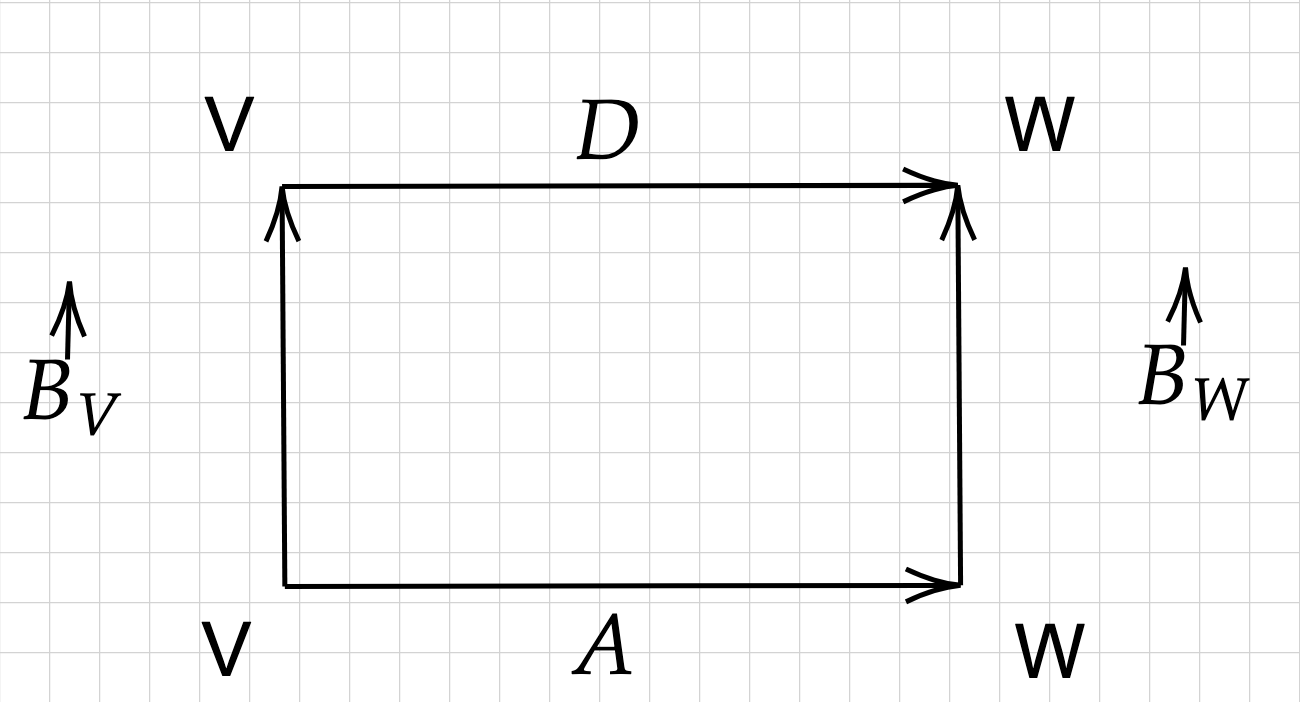
\includegraphics[width=7.5cm]{./diagram.png}
        \end{center}
        Now we wish to express the transformation $D$ w.r.t $A$. For $D$, our input vector $\mathbf{v} \in \text{Standard}$, therefore, we must first transform this vector to be in basis $B_V$.
        $$ AB_V^{-1}$$
        Then, we transform the vector (now in basis $B_W$) to the standard basis, resulting in 
        $$ D = B_WAB_V^{-1}$$
        Similarly, if we wish to express $A$ w.r.t $D$, we first recognise our input vector $\mathbf{v} \in B_V$. We must first transform this vector to the standard basis, and so
        $$ DB_V$$
        Once we are in standard basis, we now need to transform to $B_W$, and so we apply the (inverse) basis matrix
        $$ A = B_W^{-1}DB_V$$
        For change-of-basis questions, always think about
        \begin{enumerate}
            \item What basis is our input?
            \item What basis is this next transformation?
            \item What basis is our output?
        \end{enumerate}
    \end{myboxr}
    \begin{myboxr}{An alternative approach to change-of-basis, given the transformation of a basis vector} \\ 
    In some questions, you may be given a transformation defined $[T]_{B, C}$, with the bases 
    $$ B = \{e_1, e_2\}$$
    and 
    $$ C = \{f_1, f_2\}$$
    How do we find $T(f_2)$? We could of course, apply the change-of-basis to find $D$, the transformation in the standard basis 
    $$ Dv_{standard} = CTB^{-1}v_{standard}$$
    \textbf{Instead,} we can exploit the linearity of linear transformations. We first find $a$ and $b$ such that
    $$ f_2 = a \cdot e_1 + b \cdot e_2$$
    Now applying the transformation, we get 
    $$ T(f_2) = a T(e_1) + b T(e_2)$$
    Now $T(e_1), T(e_2)$ are given as linear transformations of $f_1$ and $f_2$. That is
    $$ [T]_{B, C} = \begin{pmatrix}
        t_1 & t_2 \\ t_3 & t_4
    \end{pmatrix}$$
    Implies
    $$ T(e_1) = t_1 f_1 + t_3 f_2$$
    $$ T(e_2) = t_2 f_1 + t_4 f_2$$
    And thereby, $f_2$ becomes
    $$ T(f_2) = a \cdot(t_1f_1 + t_3f_2) + b\cdot (t_2f_1 + t_4f_2)$$
    \end{myboxr}
    \begin{myboxg}{Consequences of the matrix of a linear transformation} \\ 
        Let $T : \mathbb{P}_2 \to \mathbb{R}^2$ given by $T(p) = (p(1), p(2))$ w.r.t the bases 
        $$ \{1-t, 2-t, t^2\} \text{ and }\{(2, 3), (4, 5)\}$$
        be a linear map. Find the matrix of $T$.
        \newline \\ 
        Now $T(p) = (P(1), P(2))$. The matrix
        $$ (T(1), T(t), T(t^2)) = \begin{pmatrix}
            1 & 1 & 1 \\ 1 & 2 & 4
        \end{pmatrix}$$
        Because at each basis $\{(1, 1), (t, t), (t^2, t^2) \} $
        Now $$ D = \begin{pmatrix}
            2 & 4 \\ 3 & 5
        \end{pmatrix}^{-1} \begin{pmatrix}
            1 & 1 & 1 \\ 1 & 2 & 4
        \end{pmatrix} \begin{pmatrix}
            1 & 2 & 0 \\ -1 & -1 & 0 \\ 0 & 0 &1
        \end{pmatrix}$$
        Consider the directions of the arrows - and that we must flip $\begin{pmatrix}
        2 & 4 \\ 3 & 5
    \end{pmatrix}$ to reach $D$.
    \end{myboxg}
    \begin{myboxg}{Finding $T(e_1)$ given non-standard bases and the matrix of transformation} \\
        Let $T : \mathbb{R}^2 \to \mathbb{R}$ and the standard basis 
        $$ B = \{e_1 = (1, 0), e_2 = (0, 1) \}$$ for the domain and
        $$ C = \{u_1 = (1, 4), u_2 = (1, 3) \}$$
        in the co-domain. The matrix of $T$ for these bases is
        $$ [T]_{B, C} = \begin{pmatrix}
            6 & -1 \\5 & -1
        \end{pmatrix}$$
        Find $T(e_1)$.
        \newline \\ 
        We can first find $T(e_1)$ w.r.t the basis of $C$ by simply applying 
        $$ [T]_{B, C} e_1 = \begin{pmatrix}
            6 \\ 5
        \end{pmatrix}$$
        But this is in the basis of $C$. To find it in the basis of $B$, we apply
        $$ 6 u_1 + 5 u_2 = \begin{pmatrix}
            11 \\ 39
        \end{pmatrix}$$
    \end{myboxg}
    \begin{mybox}{Nullspace and image of a linear transformation}
    \begin{enumerate}
        \item Define the terms nullspace (kernel), image, nullity and rank for a linear transformation $T: V \to W$
        \item If $A$ is a matrix, and a linear mapping is defined by $Tx = Ax$, what is the relationship between the kernel of $T$ and the kernel of $A$?
        \item What equation connects the rank and nullity of a linear map?
    \end{enumerate}
    \end{mybox}
    The \textbf{nullspace or kernel} of $T$ is defined by
    $$ \{x \in V | Tx = 0 \} = \{x \in V | Ax = 0 \} = \text{null}(A)$$
    The \textbf{image} of $T$ is defined by
    $$ \{x \in V | Ax \} = \text{col}(A)$$
    The \textbf{dimension of the kernel and image} are linked by the dimension of $V$, such that
    $$ \text{dim}(ker(T)) + \text{dim}(im(T)) = \text{dim}(V)$$
    \begin{myboxg}{Finding kernel, image, nullity and rank for the linear mappings} \\ 
        Given $T : \mathbb{R}^T \to \mathbb{R}^3$ defined by $Tx = Ax$ where
        $$ 
        A = \begin{pmatrix}
            1 & -1 & 4 & 0 & 4 \\ 2 & 1 & 7 & -1 & 11 \\ -1 & -8 & -1 & 3 & -13
        \end{pmatrix}
        $$
        find the kernel, image, nullity and rank
        \newline \\
        In echelon form, we find that
        $$ 
        A = \begin{pmatrix}
            1 & -1 & 4 & 0 & 4 \\ 0 & 3 & -1 & -1 & 3 \\ 0 & 0 & 0 & 0 & 0
        \end{pmatrix}
        $$
        The kernel of $T$ is the column space of $A$, and thus is expressed by
        $$ \text{im}(T) = \left[\begin{pmatrix}
            1 \\ 2 \\ -1
        \end{pmatrix}, \begin{pmatrix}
            -1 \\ 1 \\ -8
        \end{pmatrix}\right]$$
        The rank of $T$ is then 2, and thus the nullity is $3$. We now solve $Ax = 0$ to find the kernel of $T$.
        \newline \\  
        We parameterise $x_3, x_4, x_5 \in \mathbb{R}$ as they are non-leading columns. We find the solution
        $$
        \text{ker}(T) = \left[\begin{pmatrix}
            -11/3 \\ 1/3 \\ 1 \\ 0 \\ 0
        \end{pmatrix}, \begin{pmatrix}
            1/3 \\ 1/3 \\ 0 \\ 1\\ 0
        \end{pmatrix}, \begin{pmatrix}
            -5 \\ -1 \\ 0 \\ 0 \\ 1
        \end{pmatrix}\right]
        $$
    \end{myboxg}
    \begin{myboxg}{An example in $\mathbb{P}$} \newline 
        Given that $T: \mathbb{P}_4 \to \mathbb{R}^2, T(p) = (p(0), p'(0))$, find the kernel and image - and thus the nullity and rank.
        \newline \\ 
        Find the transformation of the standard bases
        $$ \{ 1, t, t^2, t^3, t^4 \}$$
        These become
        \begin{align*}
            T(1) &= (1, 0) \\
            T(t) &= (0, 1) \\ 
            T(\{t^2, t^3, t^4\}) &= (0, 0)
        \end{align*}
        Thereby the transformation matrix is
        $$
        T = \begin{pmatrix}
            1 & 0 & 0 & 0 & 0 \\
            0 & 1 & 0 & 0 & 0
        \end{pmatrix}
        $$
        The image is the column space, and therefore
        $$ 
        \text{im}(T) = \left\{\begin{pmatrix}
        1 \\ 0
        \end{pmatrix}, \begin{pmatrix}
        0 \\ 1
        \end{pmatrix}\right\} = \mathbb{R}^2
        $$
        And the null space is given by the solution of $Tx = 0$. A $\mathbb{P}_4$ vector is given by
        $$ a + bt + ct^2 + dt^3 + et^4$$
        It is trivial to see that $Tx = 0$ yields the solutions $a, b = 0$, and thus the kernel is
        $$ \text{span}\{t^2, t^3, t^4\}$$
        Finally, the nullity is $3$ (the dim. of the kernel) and the rank is $2$ (the dim. of the image)
    \end{myboxg}
    \subsection{Dot products, lengths and projections}
    \begin{mybox}{The definition of dot product, lengths and projections} \\ 
        The length of a vector $\mathbf{x}$ expressed by $||x||$ or $|x|$, is defined by
        $$ ||\mathbf{x}|| = \sqrt{\sum_{i=1}^nx_i}$$
        The dot product of two vectors $\mathbf{x,y}$ expressed by $\mathbf{x} \cdot \mathbf{y}$, is defined by
        $$ \mathbf{x} \cdot \mathbf{y} = \sum_{i=1}^n x_iy_i$$
        The angle $\theta$ between two vectors $\mathbf{x, y}$ expressed by
        $$ \cos \theta = \frac{\mathbf{x} \cdot \mathbf{y}}{||\mathbf{x}|| \times||\mathbf{y}||}$$
        The projection of a vector $\mathbf{x}$ onto a vector $\mathbf{y}$ is defined by
        $$ \text{proj}_{\mathbf{y}}\mathbf{x} = \frac{\mathbf{x} \cdot \mathbf{y}}{||\mathbf{y}||^2}\mathbf{y}$$
    \end{mybox}
    \subsection{The orthogonal complement}
    \begin{mybox}{The definition of an orthogonal complement} \\
        Let $V$ be a subspace in $\mathbb{R}^n$. The orthogonal complement of $V$, $V^\perp$ is defined by
        $$ V^\perp = \{\mathbf{x} \in \mathbb{R}^n | \mathbf{x} \cdot \mathbf{y} = 0 \text{ for all } \mathbf{v} \in V \}$$
        If $V$ is a plane, then $V^\perp$ is a plane perpendicular to it.
    \end{mybox}
    \begin{myboxg}{Find an orthogonal component of a plane} \\ 
        Let $W  = \{x \in \mathbb{R}^3 | 3x_1 - x_2 + 7x_3 = 0 \}$. Find $W^\perp$
        \newline \\ 
        Note that the orthogonal vector to the plane is
        $$ \begin{pmatrix}
            3 \\ -1 \\ 7
        \end{pmatrix}$$
        Thereby, $W^\complement$ is the set of vectors that are orthogonal to the plane $W$, namely
        $$ W^\perp =\left[ \begin{pmatrix} 
            3 \\ -1 \\ 7
        \end{pmatrix} \right]$$
    \end{myboxg}
    \begin{myboxg}{Find an orthogonal component of a span} \\ 
        In $\mathbb{R}^3$, let $W = \text{span}\{(1, 4, -1), (1, 2, 0)\}$. Find $W^\perp$
        \newline \\ 
        We find vectors that are orthogonal to $W$. We can find this by considering the cross product of the vectors that exist in the span. Thereby
        $$ (1, 4, -1)^T \times (1, 2, 0)^T = (2, -1, -2)^T$$
        Thereby, the orthogonal component is expressed by
        $$ W^\perp = \left[\begin{pmatrix}
            2 \\ -1 \\ -2
        \end{pmatrix} \right]$$
    \end{myboxg}
    \begin{myboxg}{A more involved example in $\mathbb{R}^4$} \\ 
        Let $W = \text{span}\{(1, -1, 2, 0), (-2, 1, 0, 1) \}$. Find $W^\perp$.
        \newline \\ 
        We then aim to find the orthogonal complement. Thereby, we find some vector(s) $\mathbf{x}$ such that
        $$ \begin{pmatrix}
            1 & -1 & 2 & 0 \\ -2 & 1 & 0 & 1
        \end{pmatrix} \begin{pmatrix}
            x_1 \\ x_2 \\ x_3 \\ x_4
        \end{pmatrix} = 0$$
        We can apply Gaussian elimination to find
        $$ \begin{pmatrix}
            1 & -1 & 2 & 0 \\
            0 & -1 & 4 & 1
        \end{pmatrix}$$
        And thereby $x_3$ and $x_4$ are parameters in $\mathbb{R}$. We find that
        $$ x_2 = 4x_3 + x_4$$
        and further
        $$ x_1 = 2x_3 + x_4$$
        Thereby, we can express the solution of the system of equations as
        $$ \begin{pmatrix}
            2x_3 + x_4 \\ 4x_3 + x_4 \\ x_3 \\ x_4
        \end{pmatrix} = x_3\begin{pmatrix}
            2 \\ 4 \\ 1 \\ 0
        \end{pmatrix} + x_4 \begin{pmatrix}
            1 \\ 1 \\ 0 \\ 1
        \end{pmatrix}$$
        and thereby the orthogonal component can be expressed as
        $$ W^\perp = \text{span}\{(2, 4, 1, 0), (1, 1, 0, 1)\}$$
    \end{myboxg}
    \subsection{Projections onto higher dimensional surfaces}
    Let $x \in \mathbb{R}^n$ and $W \subset \mathbb{R}^n$ as a subspace. We denote $o = P_Wx$ as the projection of $x$ on the subspace $W$. We say that $o$ is a projection of $x$ on $W$ iff
    \begin{enumerate}
        \item $o \in W$
        \item $x - o \in W^\perp$
    \end{enumerate}
    \begin{myboxg}{Finding a projection onto a higher dimensional surface (plane)} \newline 
    Find the projection of a vector $v = (6, 1, -5)$ onto the plane $W = \{w_1, w_2 \}$ where $w_1 = (1, 2, 1)$ and $w_2 = (-1, 1, 0)$.
    \newline \\ 
    First consider that the vector space $W + W^\perp$ consists of the entire domain, and thus we can express $v$ as
    $$ v = a_1w_1 + a_2w_2 + a_3w^\perp_3$$
    such that $w_1, w_2 \in W$, $w_3 \in W^{\perp}$. Thus, the projection of $v$ onto $W$ is expressed as
    $$ \text{proj}_Wa = a_1w_1 + a_2w_2$$
    We can take the dot product with $w_1, w_2$ to obtain a system of equations.
    \begin{align*}
        v \cdot w_1 &= a_1w_1 \cdot w_1 + a_2w_2 \cdot w_1 = 3\\ 
        v \cdot w_2 &= a_1w_1 \cdot w_2 + a_2w_2 \cdot w_2 = -5
    \end{align*}
    What occurs to the $w_3$ term? Well since $w_1, w_2 \in W$ and $w_3 \in W^\perp$, we have that $w_1\cdot w_3, w_2\cdot w_3 = 0$.
    \newline \\ 
    We then further find
    \begin{align*}
        w_1 \cdot w_1 &= 6 \\ 
        w_1 \cdot w_2 &= 1 \\
        w_2 \cdot w_2 &= 2
    \end{align*}
    Now, we can substitute our findings to get
    \begin{align*}
        3 &= 6a_1 + a_2 \\ 
        -5 &= a_1 + 2a_2
    \end{align*}
    Which we then find that $a_1 = 1, a_2 = -3$.
    \end{myboxg}
    \begin{mybox}{Orthonormal} \\   
        A set of vectors is \textbf{orthonormal} if the vectors are all of unit length and perpendicular to eachother.
        \newline \\ 
        That is for $ V = \{v_1, v_2, \dots, v_n\}$, $V$ is orthonormal if
        $$ v_i \cdot v_j = \begin{cases}
            1 & \text{if } i = j \\ 
            0 & \text{otherwise }
        \end{cases}$$
    \end{mybox}
    \begin{myboxr}{Theorem of orthonormal basis and projections}
        Let $W$ be a subspace of $V$, and suppose that $\{w_1, \dots, w_n\}$ is an orthonormal basis for $W$. The projection of any $v$ onto $W$ is given by
        $$ \text{proj}_WV = (v \cdot w_1)w_1 + \dots + (v \cdot w_n)w_n$$
    \end{myboxr}
    \begin{myboxg}{Using orthonomal basis to find a projection} \\ 
        The three vectors
        \begin{align*}
            w_1 &= \frac{1}{2}(1, 1, 1, -1) \\
            w_2 &= \frac{1}{2}(1, -1, 1, 1) \\ 
            w_3 &= \frac{1}{2}(-1, 1, 1, 1)
        \end{align*}
        form an orthonormal basis for a subspace $W \subset \mathbb{R}^4$. Find the projection onto $W$ for a vector $v = (2, 7, -1, 6)$.
        \newline \\ 
        Referring to the theorem stated above, we find
        $$
            \text{proj}_W v = \left[\begin{pmatrix}
                2 \\ 7 \\ -1 \\ 6
            \end{pmatrix} \cdot \begin{pmatrix}
                1/2 \\ 1/2 \\ 1/2 \\ -1/2
            \end{pmatrix}\right] \begin{pmatrix}
                1/2 \\ 1/2 \\ 1/2 \\ -1/2
            \end{pmatrix} + \dots
        $$
        This results in
        $$
            \text{proj}_Wv = \begin{pmatrix}
                -6/4 \\ 11 / 4 \\ 11 / 4 \\ 9/4
            \end{pmatrix}
        $$
    \end{myboxg}

    \subsection{More about the orthogonal component}
    Notice that $W^\perp = Null(A^t)$, Where $A = (b_1, b_2)$ with $b_i$ as columns. We can express
    that this is true by the following.
    \newline \\ 
    Suppose $A \in V$ is spanned by $b_1$ and $b_2$. For some arbitrary vector $\mathbf{x} \in V$, it 
    must be true that
    $$
    \begin{pmatrix}
        b_{11} \\ \dots \\ b_{1n}
    \end{pmatrix} \begin{pmatrix}
        x_1 \\ \dots \\ x_n
    \end{pmatrix} = 0
    $$
    and the same for $b_2 \cdot \mathbf{x}$. $A$ is expressed as the two column vectors
    $$
    A = \begin{pmatrix}
        b_{11} & b_{21} \\ \dots & \dots \\b_{1n} & b_{2n}
    \end{pmatrix}
    $$
    and therefore $A^T\mathbf{x} = 0$ (the nullspace of $A^T$) represents both $b_1\mathbf{x} = 0$ and $b_2\mathbf{x} = 0$.

    \begin{mybox}{Orthogonal components, projections and some theorems}
        \begin{enumerate}
            \item $Col(A)^\perp = Null(A^T)$
            \item $Null(A)^\perp = Col(A^T)$
        \end{enumerate}
        We can prove these by applying the transpose and orthogonal components in a specific order 
        \begin{align*}
            Col(A^t)^\perp &= Null(A^{T^T}) = Null(A) \\
            Col(A^t)^{\perp^\perp} &= Null(A)^\perp \\
            Col(A^t) &= Col(A^t)
        \end{align*}
    \end{mybox}
    \begin{myboxg}{Identities regarding the projection} \\ 
        The projection of $y$ of $v$ onto $CS(A)$, where $A$ has basis $W$ has two properties
        \begin{enumerate}
            \item $y$ is in $CS(A)$
            \item $v - y$ is perpendicular to $CS(A)$
        \end{enumerate}
        The first observation means that $y = Ax$ for some $x \in \mathbb{R}^m$. 
        \newline \\
        The second observation means that we must find some $x$, such that $A^T(v - Ax) = 0$, that is
        $$ A^Tv = Ax$$
        $A^TA$ is indeed invertible, and thus has a unique solution. Thereby, we have a formula for the projection onto a column space, such that
        $$ proj_Wv = y = Ax = A(A^TA)^{-1}A^Tv$$
    \end{myboxg}
    \begin{myboxr}{Linearly independence of $A$ and invertibility of $A^TA$} \\ 
        If the columns of $A$ are linearly independent, then $A^TA$ is invertible.
    \end{myboxr}
    \begin{mybox}{The projection as a linear transformation} \\ 
        \textbf{Theorem.} If $W$ is a subspace of $\mathbb{R}^n$, then the \textbf{projection map} onto $W$ is a linear transformation. Its 
        matrix wioth respect to the standard basis in $\mathbb{R}^n$ is
        $$ A(A^TA)^{-1}A^T$$ 
        where the columns of $A$ form a basis for $W$.
    \end{mybox}
    \begin{myboxg}{Proof of the projection matrix} \\
        For some matrix $A$ which columns are a basis for $W$, and some vector $c$, we wish to find the projection 
        such that
        $$ \text{proj}_Wc = Av$$
        for some arbitrary vector $v \in \mathbb{R}^n$. We then get the \textbf{perpendicular component}
        $$ c - Av$$
        The perpendicular component must, of course, be perpendicular to all the columns of $A$. Therefore
        $$ A^T(c - Av) = \mathbf{0}$$
        Now, expanding for $v$
        $$ A^TAv = A^Tc$$
        and thus $v = (A^TA)^{-1}A^Tc$. Therefore, our projection is given by
        $$ \text{proj}_Wv = A(A^TA)^{-1}A^Tc$$
        and the projection matrix is $A(A^TA)^{-1}A^T$.
    \end{myboxg}
    \begin{myboxg}{Applying the projection as a linear transformation} 
        Consider $W = Span\{(1,0,1,0), (0, 2, -1, 1) \}$ is a subspace of $\mathbb{R}^4$. Find the projection of $(2, 5, 6, 3)$ on $W$ using two methods.
        \newline \\ 
        We can apply the usual methods, of defining the projection as some linear combination of the span and the orthogonal component.
        \newline \\
        Alternatively, we use the linear transformation method.
        $$
        A^TA = \begin{pmatrix}
            1 & 0 & 1 & 0 \\ 0 & 2 & -1 & 1
        \end{pmatrix} \begin{pmatrix}
            1 & 0 \\ 0 & 2 \\ 1 & -1 \\ 0 & 1
        \end{pmatrix} = \begin{pmatrix}
            2 & -1 \\ -1 & 6
        \end{pmatrix}
        $$
        Now, computing the inverse we find that
        $$
        (A^TA)^{-1} = \frac{1}{11}\begin{pmatrix}
            6 & 1 \\ 1 & 2
        \end{pmatrix}
        $$
        And then, we find that
        $$
        A(A^TA)^{-1}A^T = \frac{1}{11}\begin{pmatrix}
            6 & 2 & 5 & 1 \\ 
            2 & 8 & -2 & 4 \\
            5 & -2 & 6 & -1 \\
            1 & 4 & -1 & 2
        \end{pmatrix}
        $$
        and then applying this to the vector we are projecting
        $$
        A(A^TA)^{-1}A^T \begin{pmatrix}
            2 \\ 5 \\ 6 \\ 3
        \end{pmatrix} = \begin{pmatrix}
            5 \\ 4 \\ 3 \\ 2
        \end{pmatrix}
        $$
    \end{myboxg}
    What about if $A$ is an orthonormal basis of $W$?
    \begin{myboxr}{Orthonomal basis and the projection transformation} \\ 
        Suppose that the columns of $Q$ form an orthonormal basis for a subspace of $W \in \mathbb{R}^n$. Then
        $$ \text{proj}_Wv = QQ^Tv$$
        for all $v \in \mathbb{R}^n$.
        \newline \\ 
        The above is a byproduct of the fact that $Q^TQ = I$.
    \end{myboxr}
    \textbf{But how do we form orthonormal bases?}
    \begin{mybox}{The Gram-Schmidt Procedure} \\ 
        The Gram-Schmidt procedure takes a basis, and then converts it to an orthonormal basis. Given a basis 
        $$ \{x_1, x_2, \dots\}$$
        \begin{enumerate}
            \item Let $v_1 = x_1$
            \item Let $v_2 = x_2$ with the component in the $v_1$ direction removed. Then, $v_2 \cdot v_1 = 0$.
            \item Let $v_3 = x_3$ with the components in the $v_1$ and $v_2$ directions removed. Then $v_3 \cdot v_2 = v_3 \cdot v_1 = 0$
            \item and so on...
            \item finally, an orthonormal basis $\{u_1, u_2, \dots \}$ is obtained by normalising (making them unit vectors) $\{v_1, v_2, \dots\}$
        \end{enumerate}
        In other words, step 2 means that
        $$ v_2 = x_2 - proj_{v_1}x_2$$
        Furthermore, step 3 means that
        $$ v_3 = x_3 - proj_{v_1}x_3 - proj_{v_2}x_3$$
        So we find the 'components of direction' by using projections.
    \end{mybox}

    \subsection{The QR factorisation}
    \begin{mybox}{QR factorisation} \\ 
        Let $A$ be an $m \times n$ matrix whose columns are linearly independent. Then $A$ can be written in the form
        $$ A = QR$$
        where:
        \begin{itemize}
            \item $Q$ is an $m \times n$ matrix with orthonormal columns
            \item $R$ is an $n \times n$ upper triangular matrix whose diagonal elements are non-zero
        \end{itemize}
    \end{mybox}
    \begin{myboxg}{QR factorisation of a basis} \\ 
        Use the Gram-Schmidt algorithm to find a QR factorisation of the matrix

        $$ A = \begin{pmatrix}
            1 & 1 & 8 \\ 2 & -2 & 7 \\ -4 & 5 & -4 \\ -2 & 1 & -6
        \end{pmatrix}$$
        \newline 
        We essentially have three linearly independent $\mathbb{R}^4$ vectors such that $A = \{x_1, x_2, x_3\}$. So we assign:
        $$v_1 = x_1 = \begin{pmatrix}
            1 \\ 2 \\ -4 \\ -2
        \end{pmatrix}$$
        $$ v_2 = x_2 - \text{proj}_{v_1}x_2 = x_2 - \frac{x_2\cdot v_1}{v_1\cdot v_1} v_1 = \begin{pmatrix}
            2 \\ 0 \\ 1 \\ -1
        \end{pmatrix}$$
        $$ v_3 = x_3 - \text{proj}_{v_2}x_3 - \text{proj}_{v_1}x_3 = \begin{pmatrix}
            0 \\ 3 \\ 2 \\ 1
        \end{pmatrix}$$
        We now find the unit vectors of $v_1, v_2, v_3$.
        $$
        u_1 = \frac{v_1}{||v_1||} = \begin{pmatrix}
            1 \\ 2 \\ -4 \\ -2
        \end{pmatrix} \cdot \frac{1}{5}
        $$
        $$
        u_2 = \frac{v_2}{||v_2||} = \begin{pmatrix}
            2 \\ 0 \\ 1 \\ -1
        \end{pmatrix} \cdot \frac{1}{\sqrt{6}}
        $$
        $$
        u_3 = \frac{v_3}{||v_3||} = \begin{pmatrix}
            0 \\ 3 \\ 2 \\ 1
        \end{pmatrix} \cdot \frac{1}{\sqrt{14}}
        $$
        Now we wish to express $A$ in terms of $u_i$.
        So
        \begin{enumerate}
            \item $x_1 = v_1 = u_1 ||v_1||$
            \item $x_2 = v_2 - v_1 = u_2||v_2|| - x_1||v_1||$
            \item $x_3 = v_3 + 2v_1 + 3v_2 = u_3||v_3|| + 2u_1||v_1|| + 3u_2||v_2||$
        \end{enumerate}
        The above relationships are found by resolving the projections.
        Therefore, we have
        $$ 
        A = \begin{pmatrix}
            u_1 & u_2 & u_3
        \end{pmatrix} \begin{pmatrix}
            ||v_1|| & -||v_1|| & 2||v_1|| \\ 
            0 & ||v_2|| & 3||v_2|| \\ 
            0 & 0 & ||v_3||
        \end{pmatrix}
        $$
        \textbf{Alternatively, we can use the fact that $Q$ is orthonormal to find $R$ with $Q$ and $A$}
        \begin{align*}
            A &= QR \\
            Q^TA &= Q^TQR \\ 
            Q^TA &= R
        \end{align*} 
    \end{myboxg} 
    \section{Least squares problems}
    First, let us motivate the least squares problem. We often wish to find $Ax = v$, for some matrix $A$ and some given vector $v$. However, a solution does not always exist.
    \newline \\
    Thereby we try to find a solution such that the distance between $Ax$ and $v$ are minimised.
    \begin{mybox}{The definition of least squares problems} \\ 
        Let $W$ be an $m$-dimensional subspace of $\mathbb{R}^n$. We can confirm the formula found above for the matrix of the projection onto $W$ by observing that $\text{proj}_{W}v$ is the closest vector of $W$ to $v$.
        \newline \\ 
        As usual we take $A$ to be an $n \times m$ matrix whose columns form a basis for $W$, such that $W = \text{CS}(A)$. Then any vector in $W$ has the form $Ax$ for some $x$ in $\mathbb{R}^m$. \\ \\
        \begin{myboxr}{The task}
            The task is to find $x$ such that $||Ax - v||$ is a minimum.
        \end{myboxr}
    \end{mybox}
    \begin{myboxg}{The shortest distance} \\ 
        The shortest distance from a vector $y$ to a subspace $W$ is the length of the vector $y - \text{proj}_W{y}$. For $W \subset \mathbb{R}^n, y \in \mathbb{R}^n$ we have
        $$ \min_{x\in W}||x - y|| = ||y - \text{proj}_{W}(y)||$$
    \end{myboxg}
    \begin{myboxr}{The least squares theorem} \\
        Let $A$ be an $n\times m$ matrix having linearly independent columns, and let $b$ be in $\mathbb{R}^n$. The vector $x$ in $\mathbb{R}^m$ which minimises $||Ax - b||$ is given by
        $$ A^TAx = A^Tb$$
    \end{myboxr}
    The least squares theorem is fundamentally deriven from projections. The 'error' from the column space, $v - Ax$ should be orthogonal to $\text{Col}(A) = A^T$, and thereby we have
    \begin{align*}A^T(v - Ax) &= 0 \\ A^TAx &= A^Tv\end{align*}
    \begin{myboxg}{An example of find $Ax = b$} \\ 
        Find the least squares solution of $Ax = b$ where
        $$ A = \begin{pmatrix}
            1 & 1 \\ 1 & 2 \\ 1 & 3 \\ 1 & 4
        \end{pmatrix}$$
        and 
        $$ b = \begin{pmatrix}
            7 \\ 4 \\ 0 \\ 2
        \end{pmatrix}$$
        Hence find the projection of $b$ onto $CS(A)$.
        \newline \\ 
        First we find $A^TA$.
        $$ A^TA = \begin{pmatrix}
            4 & 10 \\ 10 & 3
        \end{pmatrix}$$
        and $A^Tb$
        $$ A^Tb = \begin{pmatrix}
            13 \\ 23
        \end{pmatrix}$$
        Thereby, we have the equation
        $$
        \begin{pmatrix}
            4 & 10 \\ 10 & 30
        \end{pmatrix} \begin{pmatrix}
            x_1 \\ x_2
        \end{pmatrix} = \begin{pmatrix}
            13 \\ 23
        \end{pmatrix}
        $$  
        This can be found my Gaussian elimination (or the use of an inverse matrix) to find
        $$
        x = \begin{pmatrix}
            8 \\ -1.9
        \end{pmatrix}
        $$
        Thereby the 'projection' is $Ax$, such that
        $$
        Ax = \begin{pmatrix}
            1 & 1 \\ 1 & 2 \\ 1 & 3 \\ 1 &4
        \end{pmatrix}\begin{pmatrix}
            8 \\ -1.9
        \end{pmatrix} = \begin{pmatrix}
            6.1 \\ 4.2 \\ 2.3 \\ 0.4
        \end{pmatrix}
        $$
    \end{myboxg}
    \begin{myboxg}{A line-of-best fit example} \\
        Find the line $y = a + bx$ of best fit for the data points
        $$ (-1, -2), (0, -3), (1, 2), (3, 5)$$
        Plugging these values in, we find
        \begin{align*}
            -2 &= a - b \\ 
            -3 &= a \\
            2 &= a + b \\
            5 &= a + 3b
        \end{align*}
        Now we have $Ax = b$, which becomes
        \begin{align*}
        Ax &= b \\
        \begin{pmatrix}
            1 & -1 \\ 1 & 0 \\ 1 & 1 \\ 1 & 3
        \end{pmatrix} \begin{pmatrix}
            a \\ b
        \end{pmatrix} &= \begin{pmatrix}
            -2 \\ -3 \\ 2  \\ 5
        \end{pmatrix}
    \end{align*}
    The system of least squares is given by
    $$ A^TAx = A^Tb$$
    We find
    $$ A^TA = \begin{pmatrix}
        4 & 3 \\ 3 & 11
    \end{pmatrix}$$
    $$ A^Tb = \begin{pmatrix}
        2 \\ 19
    \end{pmatrix}$$
    Now we have the least-squares system of equations
    $$
    \begin{pmatrix}
        4 & 3 \\ 3 & 11
    \end{pmatrix} \begin{pmatrix}
        a \\ b
    \end{pmatrix} = \begin{pmatrix}
        2 \\ 19
    \end{pmatrix}
    $$
    Which resolves to the answer
    $$
    \begin{pmatrix}
        a \\ b
    \end{pmatrix} = \begin{pmatrix}
        4 & 3 \\ 3 & 11
    \end{pmatrix}^{-1} \begin{pmatrix}
        2 \\ 19
    \end{pmatrix} = \begin{pmatrix}
        -1 \\ 2
    \end{pmatrix}
    $$
    \end{myboxg}
    \subsection{Inner product}
    \begin{mybox}{Definition of an inner product} \\ 
        Let $V$ be a vector space over the field of real numbers. An inner product on $V$ is a function which assigns to any two vectors $u, v$ in $V$ a real number $<u, v>$ which has the following properties:
        \begin{enumerate}
            \item It is symmetric, $<u, v> = <v, u>$
            \item It preserves addition $<u_1 + u_2, v> = <u_1, v> + <u_2, v>$
            \item It preserves scalar multiplication $<\lambda u, v> = \lambda <u, v>$
            \item It is positive definite $<u, u> \ge 0$; such that $<u, u> = 0 : u = 0$.
        \end{enumerate}
    \end{mybox}
    We know of some inner products already
    \begin{enumerate}
        \item If we let $V = \mathbb{R}^n$, and let $<u, v>$ be the ordinary dot product
        $$ <u, v> = u \cdot v $$
        Then all the conditions of the definition are satisfied, so $<u, v>$ is an inner product on $\mathbb{R}^n$.
        \item Let $V$ be the vector space of all continuous functions on $[-\pi, \pi]$. We define the inner product to be
        $$ <f, g> = \frac{1}{\pi} \int_{-\pi}^{\pi} f(x)g(x)dx$$
        The first three conditions are simple to prove under linearity. The difficult identity to prove is
        $$ \frac{1}{\pi}\int_{-\pi}^{\pi}f(x)^2dx > 0$$
        whenever $f$ is not identitically zero. Consider the graph of $y = f(x)^2$. This graph never goes below the x-axis; therefore, the area under $y = f(x)^2$ must always be positive.
    \end{enumerate}
    \begin{myboxr}{Inner product definition of magnitude} \\ 
        Let $V$ be a real vector space on which an inner product $<u, v>$ has been defined. The norm or magnitude of any vector $v \in V$ is defined by
        $$ ||v|| = \sqrt{<v, v>}$$
    \end{myboxr}
    \begin{myboxg}{Examples of norms on inner products}
        \begin{enumerate}
            \item If $V = \mathbb{R}^2$ and $<u, v> = u \cdot v$, then $||v||$ is just the usual magnitude of $v$. For example 
            $$ ||(1, 2)|| = \sqrt{<(1, 2), (1, 2)>} =\sqrt{5}$$
            \item If an inner product for functions on $[-\pi, \pi]$ is given by $<f, g> = \frac{1}{\pi} f(x)g(x)dx$, then
            $$||\sin x|| = \sqrt{\frac{1}{\pi}\int_{-\pi}^{\pi} sin^2 dx} = 1 $$
            (By using the conversion $\sin x = (1 + \cos 2x) / 2$)
        \end{enumerate}
    \end{myboxg}
    \begin{mybox}{Cauchy-Schwartz Inequality} \\ 
        Let $V$ be a real vector space on which an inner product has been defined. For any $u, v \in V$, we have
        $$ |<u, v>| \le ||u|| \cdot ||v||$$
    \end{mybox}
    \begin{myboxr}{Proof of Cauchy-Schwartz}
        Let $t \in R$. Using the inner product axioms we have
        \begin{align*}
            ||tu + v||^2 &= <tu + v, tu + v> \\
            &= t^2<u, u> + 2t<u, v> + <v, v> \\ 
            &= t^2||u||^2 + 2t<u, v> + ||v||^2 \ge 0
        \end{align*}
        The discriminant is
        $$ 4<u, v>^2 - 4||u||^2||v||^2 \le 0$$
        which from there, we arrive to the Cauchy-Schwartz inequality
        $$ |<u, v>| \le ||u||^2 \cdot ||v||^2$$
    \end{myboxr}
    \begin{mybox}{Triangle inequality} \\ 
        In a vector space $V$ with an inner product
        $$||u + v|| \le ||u|| + ||v||$$
        for all $u, v$.
    \end{mybox}
    \begin{myboxr}{Proof of triangle inequality}
        \begin{align*}
            ||u+v||^2 &= <u+v, u+ v> \\
            &= ||u||^2 + 2<u, v> + ||v||^2  \\
            &\le ||u||^2 2+ 2||u|| ||v|| + ||v||^2 \\
            &\text{Above, we apply Cauchy-Scwhartz} \\
            &\le (||u|| + ||v||)^2
        \end{align*}
    \end{myboxr}
    \begin{myboxg}{Finding orthonormal basis w.r.t non-standard inner products} \\
        Find an orthonormal basis of $P_2$ with respect to the inner product
        $$ <p, q> = p(0)q(0) + p(1)q(1) + p(2)q(2)$$
        We have the standard basis
        $$ \{1, t, t^2 \}$$
        And using the Gram-Schmidt algorithm, we get
        $$
        v_1 = 1
        $$
        $$
        v_2 = t - \text{proj}_{v_1}t = t - 1
        $$
        $$
        v_3 = t^2 - \text{proj}_{v_1}t^2 - \text{proj}_{v_2}t^2 = t^2 - 5 
        $$
        Importantly, our projection definitions changed from our usual definitions, such that
        $$ 
        \text{proj}_{u}v = \frac{<u, v>}{<v, v>}v
        $$
        Thereby, we have:
        \begin{align*}
            v_1 &= 1 \\
            v_2 &= t - 1 \\ 
            v_3 &= t^2 - 2t + \frac{1}{3}
        \end{align*}
        But we require an orthonormal basis, thereby
        \begin{align*}
            u_1 &= \frac{v_1}{||v_1||} = \frac{1}{\sqrt{3}}\\
            u_2 &= \frac{v_2}{||v_2||} = \frac{t - 1}{\sqrt{2}}\\
            u_3 &= \frac{v_3}{||v_3||} = \frac{t^2 - 2t + 1/3}{\sqrt{2/3}}
        \end{align*}
    \end{myboxg}
    Therefore, a defined inner product may change (or add) definitions to what we conventionally see as the dot product.
    \subsection{Reflections}
    \begin{mybox}{Reflections}
        Let a plane $W \subset \mathbb{R}^3$, a vector $v \in \mathbb{R}^3$ and the reflection $T(v)$ of $v$ in $W$. The point on $W$ is $w$. We have
        $$ T(v) - w = -(v - w)$$
        Solving and noting that $w$ is the projection of $v$ onto $W$, we obtain
        $$ T(v) = 2w - v = 2(proj_W v) - v$$
        We can further use least squares to express in terms of the projection
        \begin{align*}
            T(v) &= 2A(A^TA)^{-1}A^Tv - v \\
            &= (2A(A^TA)^{-1}A^T - I)v
        \end{align*}
        We can extend this expression using the normal. Take $d$ to be the normal in zero on the plane $W$. Then 
        $$ T(v) = v - 2proj_d v$$
        Once we can write $proj_dv = d\frac{d\cdot v}{d\cdot d} = \frac{dd^tv}{d\cdot d}$, we have
        $$ T(v) = (I - \frac{2}{d\cdot d}dd^T)v$$
        So we can express it in terms of a single vector, $d$.
    \end{mybox}
    \begin{myboxr}{Theorem of orthogonal components and reflections} \\ 
        Let $d \in \mathbb{R}^n$ and let 
        $$ W = \{w \in \mathbb{R}^n | w \perp d \}$$
        be the orthogonal component of $span\{d\}$. For each $v \in \mathbb{R}^n$, let $T(v)$ be the reflection of $v \in W$. Then $T$ is a linear transformation, and its matrix w.r.t the standard basis of $\mathbb{R}^n$ is
        $$ Q = I - \frac{2}{d \cdot d}dd^T$$
        where $d$ is written as a column vector.
    \end{myboxr}
    \begin{myboxg}{Finding the reflection of a vector on a plane} \\
        Find the reflection of the vector $v = (6, 5, -1)$ in the plane $x_1 - 3x_2 - 2x_3 = 0$.
        \newline \\ 
        So we have the normal 
        $$ d = \begin{pmatrix}
            1 \\ -3 \\ -2
        \end{pmatrix}$$
        Therefore, our transformation matrix is
        $$ Tv = \left(I - \frac{2}{d\cdot d}dd^T\right)v$$
        Now 
        $$ dd^T = \begin{pmatrix}
            1 \\ -3 \\ -2
        \end{pmatrix}\begin{pmatrix}
            1 & -3 & -2
        \end{pmatrix} = \begin{pmatrix}
            1 & -3 & -2 \\ -3 & 9 & 6 \\ -2 & 6 & 4
        \end{pmatrix}$$
        and $d\cdot d = 14$. Now the total transformation matrix becomes
        $$ I - \frac{2}{d\cdot d}dd^T = \frac{1}{7}\begin{pmatrix}
            6 & 3 & 2 \\ 3 & -2 & -6 \\ 2 & -6 & 3
        \end{pmatrix}$$
        Now applying the transformation, we get
        $$ \begin{pmatrix}
            7 \\ 2 \\ -3
        \end{pmatrix}$$
    \end{myboxg}
    Notice two properties of the reflection:
    \begin{enumerate}
        \item The reflection of the reflection is the original vector
        \item The length of the reflection is equal to the length of the original
    \end{enumerate}
    \begin{myboxg}{Example using the above observations} \\ 
        Find the reflection $T$ such that $T(3, 4, -5) = (-2, 6, 3)$, and one such that $T(-2, 3, 4) = (5, 2, 0)$
        \newline \\ 
        If there exists a reflection such that $T(3, 4, -5) = (-2, 6, 3)$, then:
        $$ ||T(3, 4, -5)|| = ||(-2, 6, 3)|| = \sqrt{49}$$
        But $$||(3, 4, -5)|| = \sqrt{50}$$
        therefore no reflection could exist.
        \newline \\
        Similarly, with the second transformation
        $$ ||(-2, 3, 4)|| = \sqrt{29}$$
        and
        $$ ||(5, 2, 0)|| = \sqrt{29}$$
        So we must find the reflection. The normal is given by
        \begin{align*}
         d &= T(-2, 3, 4) - (-2, 3, 4) \\
         &= (5, 2, 0) - (-2, 3, 4) \\
         &= (7, -1, -4)
        \end{align*}
        And thereby, we can declare the plane
        $$ 7x - y - 4z = 0$$
    \end{myboxg}
    \begin{myboxg}{Matrix of reflection} \\ 
        Find the matrix of reflection that interchanges $\mathbf{v} = (12, 3, -5)$ and $\mathbf{w} = (13, 0, -3)$.
        \newline \\ 
        We first validate that the norms of the two vectors are equal. If this is the case, the normal between $v$ and $w$ is given as
        $$ \mathbf{w} - \mathbf{v} = \mathbf{d} = (1, -3, 2)$$
        Now the matrix of transformation is given by
        $$ Q = I - \frac{2}{\mathbf{d}\cdot\mathbf{d}}\mathbf{d}\mathbf{d}^T$$
        which becomes
        $$ Q = \frac{1}{7}\begin{pmatrix}
            6 & 3 & -2 \\ 3 & -2 & 6 \\ -2 & 6 & 3
        \end{pmatrix}$$
        Note this is equal to $v - 2\text{proj}_dv$ in matrix form, as
        $$ \text{proj}_dv = d\frac{d\cdot v}{d\cdot d} = \frac{dd^Tv}{d\cdot d}$$
    \end{myboxg}
    \section{Determinants and their uses}
    Only square matrices have determinants. Consider the following matrices
    $$
        \begin{vmatrix}
            a & b \\ c & d
        \end{vmatrix},
        \begin{vmatrix}
            a & b & c \\ d & e & f \\ g & h & i
        \end{vmatrix}
    $$
    The determinant for the $2 \times 2$ matrix is
    $$ ad - bc$$
    and for the $3 \times 3$ matrix is
    $$ a \cdot (e\cdot i - h \cdot f) - b\cdot(d \cdot i - g \cdot f) + c \cdot (d \cdot h + g \cdot e)$$
    \begin{mybox}{Laplace transformation} \\ 
        The systematic way of finding determinants is as such. Choose a column $i$, or a row $j$ depending. Then the determinant 
        for the matrix $A$ is given by
        $$ \text{det}(A) = \sum_{j=1;i=1}^{n} (-1)^{i + j}a_{ij} \cdot \text{det}(M_{ij})$$
        where $M_{i, j}$ is the minor of $a_{ij}$, the matrix remaining when removing the $i$-th row and $j$-th column. You iterate through the 'free axis' (if you fixed the row, iterate through columns, etc).
    \end{mybox}
    \begin{myboxr}{Determinants and their relationship to $Ax = b$}
        \begin{itemize}
            \item If $det(A) \neq 0$, then $Ax = b$ has a unique solution (since $A$ is invertible)
            \item If $det(A) = 0$, then $Ax = 0$ has infinitely many solutions
            \item If $det(A) \neq 0$, then $Col(A)$ has $n$ linearly independent columns.
            \begin{itemize}
                \item Thereby, $Col(A) = \mathbb{R}^n$
            \end{itemize}
        \end{itemize}
    \end{myboxr}
    \textbf{Identities involving determinants}
    \begin{enumerate}
        \item $det(A^T) = det(A)$
        \item $det(A^{-1}) = \frac{1}{det(A)}$
        \item $det(AB) = det(A)det(B)$
        \item Two matrices $A, B$ are similarly if $A = PBP^{-1}$. Thereby $det(A) = det(B)$, as
        $$ det(A) = det(P)det(B)\frac{1}{det(P)} = det(B)$$
        \item An orthogonal matrix has $det = 1$.
        \item If there are any zero rows, then $det = 0$.
        \item A matrix with two equal rows have determinant zero
        \item Adding a multiple of a row to another row doesn't change the determinant
        \item If $B = \alpha A$ and $A \in M_{n, n}$, then $det(B) = \alpha^n det(A)$
        \item Multiplying a row by $\alpha$ in $A$ changes the determinant to $\alpha det(a)$
    \end{enumerate}
    \begin{myboxr}{Using Gaussian Elimination to simply determinants} \\ 
        Given the task of finding the determinant for
        $$
        \begin{vmatrix}
            -1 & 3 & 1 & 2 \\ 2 & -6 & 4 & 5 \\ 3 & -4 & -4 & -5 \\ 6 & -8 & -2 & 9
        \end{vmatrix}
        $$
        This at first appears to be a long task. However, we can use gaussian elimination to reduce the 
        first column to all zeroes besides the first element - which we can then do a \textbf{reduction by rows} to do a single $3 \times 3$ determinant.
    \end{myboxr}
    \section{Eigenvalues and eigenvectors}
    \begin{mybox}{Defining the eigen-(value and vector)} \\ 
        A complex number $\lambda$ is called an eigen value of a matrix $A \in M_{m, n}(\mathbb{C})$, if there is a non-zero vector $x \in \mathbb{C}^n$ such that $Ax = \lambda x$. In this case, we call $x$ an eigenvector of the eigenvalue $\lambda$.
        \newline \\ 
        Now since 
        $$ (A - \lambda I)x = 0$$
        is necessary for the existence of an eigen-value/vector, we then have that
        $$ det(A - \lambda I) = 0$$
    \end{mybox}
    \begin{myboxr}{Characteristic polynomial} \\ 
        The characteristic polynomial is defined by
        $$ P(x) = det(A - \lambda I)$$
        Solving for $P(x) = 0$ yields the eigenvalues.
    \end{myboxr}
    \textbf{Characteristics of eigenvalues and vectors}
    \begin{enumerate}
        \item For an $n \times n$ matrix - there are $\le n$ eigenvalues.
        \item $det(A)$ is the product of eigenvalues.
    \end{enumerate}
    \begin{myboxg}{A $2 \times 2$ example} \\ 
        Find the eigenvalues and the corresponding eigenvectors of the matrix
        $$ A = \begin{pmatrix}
            -8 & -5 \\ -9 & 4
        \end{pmatrix}$$
        \newline \\ 
        We consider the characteristic polynomial $$ P(x) = \text{det}(A - \lambda I)$$
        Thereby, we have
        $$\begin{vmatrix}
            -8 - \lambda & -5 \\ -9 & 4 - \lambda
        \end{vmatrix} $$
        which results in $ \lambda^2 + 4\lambda - 77$, which can be factorised to
        $$ (\lambda + 11)(\lambda - 7)$$
        resulting in the eigenvalues $\lambda = -11, 7$. To find the eigenvector, we consider the nullspace of $A - \lambda I$. Consider for $\lambda = -11$
        $$\text{Null}\begin{pmatrix}
            3 & -5 \\ -9 & 15
        \end{pmatrix}  = A -  (-11I)$$
        We can Gaussian eliminate for
        $$\text{Null}
        \begin{pmatrix}
            3 & -5 \\ 0 & 0
        \end{pmatrix}
        $$
        Which results in the vector
        $$
        \begin{pmatrix}
            5/3 \\ 1
        \end{pmatrix}
        $$
        Similarly, we can do this for $\text{Null}(A - 7I)$.
    \end{myboxg}
    \begin{myboxg}{A $3\times 3$ example} \\ 
        Find the eigenvalues and the corresponding eigenvectors of the matrix
        $$ B = \begin{pmatrix}
            0 & 4 & -10 \\ 1 & 0 & 5 \\ 1 & -2 & 7
        \end{pmatrix}$$
        \newline \\ 
        This becomes more difficult as the characteristic polynomial is of degree $3$. We rely on Maple's 
        $$ \verb|p := CharacteristicPolynomial(A, z)|$$
        which finds the characteristic polynomial of $A$ in $z$. We find using this command that
        $$ P(x) = det(B - xI) = (x-2)^2(x-3)$$
        Thereby we have eigenvalues $\lambda = 2, 3$. So we find $\text{Null}(A - 2I)$, which becomes
        $$ \text{Null}(A - 2I) = \begin{pmatrix}
            1 & -2 & 5 \\ 0 & 0 & 0 \\ 0 & 0 & 0
        \end{pmatrix}$$
        Which we can then extract that $x_1 - 2x_2 + 5x_3 = 0$, and from then get the eigen vectors
        $$ \begin{pmatrix}
            2 \\ 1 \\ 0
        \end{pmatrix}, \begin{pmatrix}
            -5 \\ 0 \\ 1
        \end{pmatrix}$$
        Similarly, we can do this for $\text{Null}(A - 3I)$.
    \end{myboxg}
    \subsection{Diagonalisation and powers of matrices}
    \begin{mybox}{Diagonalisation} \\
        Let $A$ be an $n \times n$ matrix with $n$ linearly independent eigenvectors $b_1, \dots, b_n$. Then the matrix of linear transformation $T(v) = Av$ w.r.t the basis $\{b_1, b_2, \dots, b_n \} \in \mathbb{C}^n$ is \textbf{diagonal}. Writing vectors in terms of a basis of eigenvectors, then, the formula for $T$ becomes $$T\begin{pmatrix}
            x1 \\ \vdots \\ x_n
        \end{pmatrix} = D\begin{pmatrix}
            x_1 \\ \vdots \\ x_n
        \end{pmatrix} = \begin{pmatrix}
            \lambda_1x_1 \\ \vdots \\ \lambda_nx_n
        \end{pmatrix}
        $$
        We can write $A = PDP^{-1}$, where $$P = \begin{pmatrix}
            b_1 & b_2 & \dots & b_n
        \end{pmatrix}$$
    \end{mybox}
    \begin{myboxg}{A $2 \times 2$ example} \\
        Diagonalise (if possible) the matrix $A = \begin{pmatrix}
            -8 & -5 \\ -9 & 4
        \end{pmatrix}$ and hence find a formula for $A^n$. 

        $$\text{Eigenvectors} =  \begin{pmatrix}
            5 \\ 3
        \end{pmatrix}, \begin{pmatrix}
            1 \\ -3
        \end{pmatrix}$$
        with eigenvalues $-11, 7$ respectively.
        Therefore, we have the basis of eigenvectors
        $$ B = \begin{pmatrix}
            5 & 1 \\ 3 & -3
        \end{pmatrix}$$
        We know that $A =  BDB^{-1}$. $D$ is the diagonal matrix of eigenvalues corresponding to their respective vectors
        $$ D = \begin{pmatrix}
            -11 & 0 \\ 0 & 7
        \end{pmatrix}$$
        We then find that $A^n = PD^nP^{-1}$ as the $P$'s cancel out recursively. Thus
        $$ A^n = \begin{pmatrix}
            5 & 1 \\ 3 & -3
        \end{pmatrix}\begin{pmatrix}
            (-11)^n & 0 \\ 0 & 7^n
        \end{pmatrix}\begin{pmatrix}
            5 & 1 \\ 3 & -3
        \end{pmatrix}^{-1}$$
    \end{myboxg}
    \begin{myboxr}{Traces, determinants and eigenvalues} \\ 
        Given some eigenvalues $lambda_1, \dots, \lambda_n$ for a matrix $A$, we have that
        $$ \lambda_1 + \lambda_2 + \dots + \lambda_n = tr(A)$$
        \newline \\ 
        Furthermore, it holds true that
        $$ \lambda_1 \cdot \lambda_2 \dots \cdot \lambda_n = det(A)$$
    \end{myboxr}
    \begin{myboxg}{}
    \end{myboxg}
    \begin{mybox}{The eigenspace} \\ 
        Let $A$ be an $n \times n$ matrix and let $\lambda$ be an eigenvalue of $A$. The eigenspace of $A$ corresponding to $\lambda$ is
        $$ E_\lambda = \{ v \in \mathbb{C}^n | Av = \lambda v\}$$
        that is, the set of all eigenvectors of $A$ corresponding to $\lambda$, together with the zero vector.
    \end{mybox}
    \begin{myboxr}{Algebraic and geometric multiplicity} \\ 
        Consider an eigenvalue $\lambda$.
        \begin{itemize}
            \item The algebraic multiplicity of $\lambda$ is the number of times $\lambda$ occurs as a root of the characteristic polynomial
            \item The geometric multiplicity of $\lambda$ is the dimension of the eigenspace $E_\lambda$ (the null space). Found by gaussian eliminating $A - \lambda I$.
        \end{itemize}
    \end{myboxr}
    \begin{myboxr}{Geometric multiplicity $\le$ arithmetic multiplicity} \\ 
        Since arithmetic multiplicity defines the number of times an eigenvalue appears, and geometric multiplicity
        defines how many independent directions an eigenvector can take
        $$ GM \le AM$$
    \end{myboxr}
    \begin{mybox}{Theorem of geometric multiplicity and algebraic multiplicity} \\ 
        Let $A$ be an $n \times n$ matrix and $\mu$ is an eigenvalue of $A$. The geometric multiplicty of $\mu$
        is less than or equal to it's algebraic multiplicity.
        \newline \\ 
        Let $T : \mathbb{C}^n \to \mathbb{C}^n$ be the linear map given by $T(v) = Av$. Suppose that the geometric multiplicity of $\mu$ is $r$, so that $A$ has $r$ independent eigen vectors $\{v_1, \dots, v_r \}$ corresponding to the eigenvalue $\mu$. Consider an ordered basis $B = \{v_1, \dots, v_r, b_{r+1}, \dots, b_n\}$ for $\mathbb{C}^n$ beginning with these $r$ eigenvectors.
        \newline \\ 
        The matrix of transformation $M$ with respect to the basis $B$ is then
        $$ T(v_1) = Av_1 = \mu v_1, \dots, T(v_r) = Av_r = \mu v_r $$
        Therefore the first $r$ columns is a 'diagonal' matrix of the eigenvalue $\mu$ (filled with zeroes until $n$) - and the rest of the columns are something. Thereby, $A$, the matrix of transformation in standard basis is
        $$ A = BMB^{-1}$$
        Therefore
        $$ A - \lambda I = BMB^{-1} - \lambda BIB^{-1} = B(M - \lambda I)B^{-1}$$
        therefore the characteristic polynomaial of $A$ is
        \begin{align*}
            p(\lambda) &= \pm det(A - \lambda I) \\
                       &= \pm det(B)det(M -\lambda I)det(B^{-1})  \\
                       &= \pm det(M - \lambda I) \\
                       &=  (\lambda - \mu)^r \times \text{other stuff}
        \end{align*}
    \end{mybox}
    \begin{myboxr}{Diagonalisability and multiplicities} \\ 
        A matrix is diagonalisable if and only if every eigenvalue has geometric multiplicty equal to it's algebraic multiplicity
    \end{myboxr}
    \begin{myboxg}{Diagonalisabilty and multiplicity} \\ 
        Show that the vector $v = (-1, 1, 1, 0)^T$ is an eigenvector of the matrix
        $$ A = \begin{pmatrix}
            6 & -2 & 3 & 1 \\ 3 & -1 & 9 & 3 \\ -2 & 4 & -1 & -2 \\ -1 & 2 & -3 & 4
        \end{pmatrix}$$
        and find with minimal calculation all eigenvalues of $A$ and their multiplicities. Is $A$ diagonalisable?
        \newline \\ 
        If $v$ is an eigenvector, then $Av = \lambda v$ for some $\lambda$.
        $$ Av = \begin{pmatrix}
            -5 \\ 5 \\ 5 \\ 0
        \end{pmatrix}$$
        Clearly, $Av = 5v$, and thus $v$ is an eigenvector, with eigenvalue $5$. Now consider
        $$ A - 5I_4 = \begin{pmatrix}
            1 & -2 & 3 & 1 \\ 3 & -6 & 9 & 3 \\ -2 & 4 & -6 & 2 \\ -1 & 2 & -3 & -1
        \end{pmatrix}$$
        To find the dimension of the eigenvalue $\lambda = 5$. After gaussian elimination, it becomes
        $$ \begin{pmatrix}
            1 & -2 & 3 & 1  \\ 0 & 0 & 0 & 0 \\ 0 & 0 & 0 & 0 \\ 0 & 0 & 0 & 0
        \end{pmatrix}$$
        We know that the geometric multiplicty of $\lambda = 3$, and therefore the algebraic multiplicity must be $\ge 3$.
        So we know the geometric multiplicity of $\lambda = 5$ is 3. Therefore, we have eigenvalues
        $$ \{5, 5, 5, \mu \}$$
        How do we find $\mu$? We know that $\text{tr}(A) = \text{sum of eigenvalues}$. Therefore
        $$\mu + 5 \cdot 3 = 6 - 1 - 1 + 4$$
        Thereby, $\mu = -7$
        
        So alg. mult. of $\lambda = 3$, and therefore $A$ is diagonalisable.
    \end{myboxg}
    \subsection{Similarity of matrices}
    \begin{mybox}{Similarity} \\ 
        If $A$ and $B$ are similar matrices, then they have the same characteristic polynomial, the same eigen values, the same trace and the same determinant. That is:
        \begin{center}
            If $A$ and $B$ are similar matrices,, then $A = PBP^{-1}$ for some matrix $P$.
        \end{center}
    \end{mybox}
    \begin{myboxr}{Algebraic rules of similarity} \\ 
        Similarity of amtrices is an equivalence relation on $M_{nn}^{\mathbb{R}}$. That is, if $A, B$ and $C$ are $n \times n$ matrices, then
        \begin{itemize}
            \item $A$ is similar to $A$
            \item If $A$ is similar to $B$, then $B$ is similar to $A$
            \item If $A$ is similar to $B$, and $B$ is similar to $C$ then $A$ is similar to $C$.
        \end{itemize}
    \end{myboxr}
    The following are some identities of eigenvalues and eigenvectors in finite-dimensional space.
    \begin{itemize}
        \item If $T : V \to v$ is linear and $T(v) = \lambda v$ for some scalar $\lambda$ and some non-zero $v \in V$, then $\lambda$ is said to be an \textbf{eigenvalue} of $T$ and $v$ is an $\textbf{eigenvector}$ of $T$.
        \item If $T: \mathbb{C}^n \to \mathbb{C}^n$ is defined by $T(v) = Av$, then the eigenvalues and eigenvectors of $T$ are the same as those of $A$.
        \item Let $T: M_{33} \to M_{33}$, where $T(X) = X^T$. If $X$ is an eigenvector of $T$, then $X$ is no the zero matric and $T(X) = \lambda X$, that is $X^T = \lambda X$. Therefore
        $$ X = (X^T)^T = (\lambda X)^T = \lambda X^T = \lambda^2 X$$
        and since $X \ne 0$ the only possible eigenvalues are $\lambda = \pm 1$.
    \end{itemize}
    The following are some identities of eigenvalues and eigenvectors in infinite-dimensional space.
    \begin{itemize}
        \item Let $T$ be the differentiation map on the vector space $P$ of all polynomials. To find eigenvalues and eigenvectors of $T$ we must solve
        $$ \frac{dp}{dt} = \lambda p$$
        the only solution is when $p(t)$ is constant, as otherwise the left hand side and right hand side are of different degrees.
        \newline \\ 
        So the only eigenvalue is $\lambda = 0$, and the corresponding eigenvectors are the constant polynomials.
        \item Let $T$ be the differentiation map on $V$, the vector space of all differentiable functions from $\mathbb{R} \to \mathbb{R}$. Since we are no longer restricted to polynomials, the differential equation
        $$ \frac{dy}{dx} = \lambda y$$
        has solutions for every real $\lambda$ and the eigenspaces are
        $$ E_{\lambda} = \{ce^{\lambda x} | c \in \mathbb{R} \} = \text{Span}\{e^{\lambda x} \}$$
        each of which is one dimensional.
    \end{itemize}
    \begin{myboxg}{Determinant transformations} \\ 
        Let the minors associated with the first column be
        $$ M_{31} = \begin{vmatrix}
            a_1 & b_1 \\ a_2 & b_2
        \end{vmatrix}, M_{21} = \begin{vmatrix}
            a_1 & b_1 \\ a_3 & b_3
        \end{vmatrix}, M_{11} = \begin{vmatrix}
            a_2 & b_2 \\ a_3 & b_3
        \end{vmatrix}$$
        Using the minors above, write the formula for the determinant $T(\mathbf{x})$ using the co-factor expansion by the first column.
    \end{myboxg}
    \section{Orthogonal transformations}
    \begin{mybox}{Rotations in $\mathbb{R}^2$} \\ 
        Define a mapping $T : \mathbb{R}^2 \to \mathbb{R}^2$ by taking $T(x)$ to be the vector obtained by rotating $x$ through an angle $\alpha$ about the origin. Taking a little care if $\alpha$ is not a positive acute angle, we can see that
        $$ T(1, 0) = (\cos\alpha, \sin\alpha), T(0, 1) = (-\sin\alpha, \cos\alpha)$$
        Then, the matrix of rotation w.r.t the standard bases is given by
        $$ R_{\alpha} = \begin{pmatrix}
            \cos\alpha & -\sin\alpha \\ \sin\alpha & \cos\alpha
        \end{pmatrix}$$
        $R_a$ is an \textbf{orthonormal} matrix.
    \end{mybox}
    \begin{itemize}
        \item It is true that $R_\alpha^{-1} = R_{-\alpha}$
        This is as
        \begin{align*}
            R_\alpha R_{-\alpha} &= R_\alpha R_{\alpha}^T = I \\ 
            R_{\alpha}^{-1} &= R_{-\alpha}
        \end{align*}
        \item $R_\alpha$ has no real eigenvalues unless $\alpha = n\pi$
        \begin{align*}
            \text{det}(R_\alpha - \lambda I) &= 0 \\
            \lambda^2 - 2\lambda \cos\alpha + 1 &= 0 \\ 
            \lambda &= \cos\alpha  \pm i\sin\alpha \\ 
            &= e^{\pm i \alpha}
        \end{align*}
        Thereby only real when $\sin\alpha = 0 \implies \alpha = n\pi$.
        \item The condition for a matrix $R$ to be considered a \textbf{matrix of rotation} 
        is 
        \begin{enumerate}
            \item The matrix is orthonormal
            \item $\text{det}(R) = 1$
        \end{enumerate}
    \end{itemize}
    \begin{myboxg}{Showing a matrix of rotation} \\ 
        Show that the matrix
        $$ R = \frac{1}{5}\begin{pmatrix}
            3 & -4 \\ 4 & 3
        \end{pmatrix}$$
        is a matrix of rotation, and find it's angle of rotation. \\ 

        First consider orthonormality:
        $$
        \frac{1}{5}\begin{pmatrix}
            3 \\ 4
        \end{pmatrix} \cdot \frac{1}{5} \begin{pmatrix}
            -4 \\ 3
        \end{pmatrix} = 0
        $$
        Furthermore the column vectors are of magnitude $1$. Consider the determinant
        $$
            \text{det}\begin{pmatrix}
                3/5 & -4/5 \\ 4/5 & 3/5 
            \end{pmatrix} = \frac{1}{25}(9 + 16) = 1
        $$
        Now considering that $\text{tr}(R) = 2\cos\alpha$
        \begin{align*}
            2\cos\alpha &= \frac{3}{5} + \frac{3}{5}
            \cos\alpha &= \frac{3}{5} \\ 
            \alpha &= \arccos\left(\frac{3}{5}\right)
        \end{align*}
    \end{myboxg}
    \begin{myboxr}{Theorem on determinants and traces with rotations} \\ 
        An orthogonal matrix $A$ in $M_{2, 2}$ is a matrix of rotation if $\text{det}(A) = 1$. 
        \newline \\ 
        Then the rotation has an angle of cosine
        $$\cos\alpha = \frac{1}{2}\text{tr}(A) $$
        And thereby, the angle of rotation is given by
        $$ \alpha = \pm \cos^{-1}\left(\frac{1}{2}\text{tr}(A) \right)$$
    \end{myboxr}
    When is an orthogonal matrix $A$ not a matrix of rotation?
    \begin{center}
        When $\text{det}(A) = -1$
    \end{center}
    \begin{myboxg}{Finding matrices of reflection in an axis} \\ 
        Find the matrix of reflection in the axis $e_1 = (1, 0) \in \mathbb{R}^2$
        \newline \\ 
        Geometrically, this means that we are reflecting upon the $x$-axis. Like with any linear transformation, we consider
        the effects on the standard basis vectors. We have $T : \mathbb{R}^2 \to \mathbb{R}^2$, and we find $A = (T(e_1), T(e_2))$ where $e_1, e_2$ are the standard bases. We have
        $$ T(1, 0) = (1, 0)^T$$
        $$ T(0, 1) = (1, -1)^T$$
        and thereby, we have the matrix of reflection
        $$ A = \begin{pmatrix}
            1 & 0 \\ 0 & -1
        \end{pmatrix}$$
    \end{myboxg}
    \begin{mybox}{Rotations in $\mathbb{R}^3$} \\
        To describe a rotation in $\mathbb{R}^3$, you need
        \begin{enumerate}
            \item The axis - a line that stays fixed during the rotation
            \item The angle - how mcuch everything else (perpendicular to the axis) is rotated around that line
        \end{enumerate}
    \end{mybox}
    \begin{myboxr}{Finding rotations in 3D} \\
        Denote the axis of rotation by $v_1$, and choose an orthonormal basis $B = \{v_1, v_2, v_3 \}$. Then $T$ will leave $v_1$ unchanged, and will act on $v_2$ and $v_3$ like a rotation of the plane. 
        \newline \\ 
        Drawing a diagram of the plane spanned by $v_2$ and $v_3$, we can consider the matrix
        $$ R_{\alpha} = \begin{pmatrix}
            1 & 0 & 0 \\ 0 & \cos\alpha & - \sin\alpha \\ 0 & \sin\alpha & \cos\alpha
        \end{pmatrix}$$
        This fixes $v_1$ such that $T(v_1) = v_1$, and then behaves like a $\mathbb{R}^2$ rotation on the $v2 - v3$ plane. Consider that
        \begin{align*}
            T(v_1) &= v_1 \\ 
            T(v_2) &= \cos\alpha v_2 + \sin\alpha v_3 \\ 
            T(v_3) &= -\sin\alpha v_2 + \cos\alpha v_3
        \end{align*}
        Then, in the standard basis, we have the transformation
        $$ T_{standard} = BR_\alpha B^{-1}$$
    \end{myboxr}
    \begin{myboxg}{An example} \\
        Let $T$ be the rotation of $\mathbb{R}^3$ with axis $(1, 1, 1)^T$ and angle $45^{\circ}$. Find $T(1, 0, 0)$.
        \newline \\
        We can take $v_1 = \frac{1}{\sqrt{3}}(1, 1, 1)$.  Furthermore, we can take $v_2 = \frac{1}{\sqrt{2}}(0, 1, -1)$.
        $v_3$ can be decided by the cross product of $v_1$ and $v_2$, such that $v_3 = v_1 \times v_2 = \frac{1}{\sqrt{6}}(-2, 1, 1)$. Thereby, we have
        $$ B = \begin{pmatrix}
            1/\sqrt{3} & 0 & -2/\sqrt{6} \\ 
            1/\sqrt{3} & 1/\sqrt{2} & 1/\sqrt{6} \\
            1/\sqrt{3} & -1/\sqrt{2} & 1/\sqrt{6}
        \end{pmatrix}$$
        Furthermore, given $\alpha = \frac{\pi}{4}$, we have
        $$ R_\alpha = \begin{pmatrix}
            1 & 0 & 0 \\ 0 & \frac{1}{\sqrt{2}} & -\frac{1}{\sqrt{2}} \\ 
            0 & \frac{1}{\sqrt{2}} & \frac{1}{\sqrt{2}}
        \end{pmatrix}$$
        Now, we get the final transformation
        $$ BR_\alpha B^{-1}(1, 0, 0) = \frac{1}{3\sqrt{2}} \begin{pmatrix}
            2 + \sqrt{2} \\ -1 + \sqrt{2} + \sqrt{3} \\ -1 + \sqrt{2} - \sqrt{3} 
        \end{pmatrix}$$
    \end{myboxg}
    \begin{myboxr}{Showing matrices of rotation in $\mathbb{R}^3$} \\ 
        How do we
        \begin{enumerate}
            \item Tell whether a matrix is a matrix of rotation?
            \item Find the axis and angle of the rotation?
        \end{enumerate} 
        Well
        \begin{enumerate}
            \item Any $3 \times 3$ orthogonal matrix whose determinant is $+1$ is the matrix of rotation in $\mathbb{R}^3$.
            \item Let $Q$ be the matrix of rotation with axis $v$. Since $v$ is unchanged by the rotation, then
            $$ Qv = v = \lambda v$$
            therefore $\lambda = 1$. \textbf{The axis of the rotation is an eigenvector of $Q$ responsnding to $\lambda = 1$}.
            \item $tr(A) = tr(R_{\alpha}) = 1 + 2\cos\alpha$, and from this we can find the angle of rotation.
        \end{enumerate}
    \end{myboxr}
    \begin{myboxg}{Example of proving a matrix of rotation in $\mathbb{R}^3$} \\ 
        Let 
        $$ Q = \frac{1}{3}\begin{pmatrix}
            2 & 1 & -2 \\ -2 & 2 & -1 \\ 1 & 2 & 2
        \end{pmatrix}$$. Show that $Q$ is a matrix of rotation, find its axis of rotation and determine its angle of rotation.
        \newline \\ 
        We can trivially prove $Q$ is orthogonal. Consider the determinant
        $$\text{det}(Q) = \frac{1}{3^3}(15 + 12) = 1 $$
        Therefore, we have that $Q$ is a matrix of rotation. Now we find the axis and the angle of rotation. We already know 
        that the eigenvalue is $\lambda = 1$, therefore we find
        $$ Q - 1 \cdot I =\frac{1}{3}\begin{pmatrix}
            -1 & 1 & -2 \\ -2 & -1 & -1 \\ 1 & 2 & -1
        \end{pmatrix} $$
        Now, we find the null space of this matrix to find the eigenvector
        $$ (Q - I)_{\text{elim.}} = \frac{1}{3}\begin{pmatrix}
            -1 & 1 & -2 \\ 0 & -3 & 3 \\ 0 & 0 & 0
        \end{pmatrix}$$
        With the span 
        $$ z\begin{pmatrix}
            -1 \\ 1 \\ 1
        \end{pmatrix}$$
        where $z \in \mathbb{R}$. Therefore, our axis of rotation is $(-1, 1, 1)$. Now, to find the angle
        \begin{align*}
            1 + 2\cos\alpha &= \text{tr}(Q) \\ 
            1 + 2\cos\alpha &= 2 \\ 
            2\cos\alpha &= 1 \\
            \cos\alpha &= \frac{1}{2} \\
            \alpha &= \arccos\left( \frac{1}{2}\right) 
        \end{align*}
    \end{myboxg}
    Consider the following propositions
    \begin{itemize}
        \item $Qu \cdot Qv = u \cdot v$
        \item $||Qv|| = ||v||$
    \end{itemize}
    \begin{mybox}{Transforming $\text{det}(A) = -1$ to a matrix of rotation and reflection matrices} \\
        Given an orthogonal matrix $Q$ with determinant $-1$, we can utilise the matrix
        $$ M = \begin{pmatrix}
            -1 & 0 \\ 0 & 1
        \end{pmatrix}, \begin{pmatrix}
            -1 & 0 & 0 \\ 0 & 1 & 0 \\ 0 & 0 & 1
        \end{pmatrix}$$
        and find that since $M^2 = I$ and $M^{-1} = M$, that
        $$ QM$$
        is a orthogonal matrix with $\text{det}(QM) = 1$
        \newline \\ 
        Write $R = QM$, such that $R$ is a rotation matrix, we have
        $$ Qv = RMv$$
        and $Q$ can be broken up into two stages.
        \begin{enumerate}
            \item First, $v$ is transformed to $Mv$, which means that the first component of $v$ changes signs
            \item Second, the resulting vector $Mv$ is rotated through some angle $\alpha$ through axis $z$
        \end{enumerate}
        \begin{center}
            An orthogonal matrix with determinant $-1$ represents a reflection in a plane followed by a rotation.
        \end{center}
    \end{mybox}
    \begin{myboxr}{Finding the plane of reflection and the angle of reflection} \\
        If $v$ is the normal to the plane, then $Qv = -v = \lambda v$, and since $\lambda = -1$, we find the eigenvector $v$ with eigenvalue $-1$ of $Q$.
    \end{myboxr}
    \begin{myboxg}{Finding the matrix of reflection, plane of reflection and angle of rotation} \\ 
        Let 
        $$ Q = \frac{1}{9}\begin{pmatrix}
            4 & -7 & -4 \\ 1 & -4 & 8 \\ 8 & 4 & 1
        \end{pmatrix}$$
        Show that $Q$ is a matrix of reflection, find its plane of reflection and the angle of rotation around its normal.
        \newline \\
        Note that $\text{det}(Q) = -1$. We find the eigenvector such that $\lambda = -1$, then use this to find the angle of rotation. So we find $\text{Null}(Q + I)$ such that 
        \begin{align*}
        \text{Null}(Q + I) &= \text{Null}\begin{pmatrix}
            1 & 5 & 8 \\ 0 & 2 & 3 \\ 0 & 0 & 0
        \end{pmatrix} \\ 
        &= \text{span}\left\{ \begin{pmatrix}
        -1 \\ -3 \\ 1
        \end{pmatrix} \right\}
        \end{align*}
        And thereby the axis of rotation is $(-1, -3, 1)^T$ and the plane of reflection is $-x - 3y + z = 0$. To find the angle 
        of rotation, we have that
        \begin{align*}
            \text{tr}(Q) &= -1 + 2\cos\alpha \\
            \frac{1}{9} &= -1 + 2\cos\alpha \\
            2\cos\alpha &= \frac{10}{9} \\ 
            \alpha &= \arccos\left(\frac{5}{9}\right)
        \end{align*}
    \end{myboxg}
    \begin{myboxr}{Finding the angle of rotation with matrices of $\text{det}(A) = -1$ (matrix of reflection)} \\ 
        Choose an orthonomal basis with $v = \{v_1, v_2, v_3\}$ where $v_1$ is the axis of rotation (found by $\lambda = -1$). The matrix of $Q$ has a matrix of rotation $$R_{\alpha}^{-} = \begin{pmatrix}
            -1 & 0 & 0 \\ 0 & \cos\alpha & -\sin\alpha \\ 0 & \sin\alpha & \cos\alpha
        \end{pmatrix}$$
        Since $Q$ and $R_{\alpha}^{-}$ are matrices of the same transformation with respect to different bases, they have teh same trace
        $$\text{tr}(Q) = \text{tr}(R_{\alpha}^{-}) = -1 + 2\cos\alpha$$
    \end{myboxr}
    \begin{mybox}{Pure reflections} \\
        If $\alpha = 0$, and $Q$ is a matrix of reflection, then it is a \textbf{pure reflection}.
    \end{mybox}
    \subsection{Applications of diagonalisation to geometry}
    \begin{mybox}{Connections between diagonalisation and linear algebra} \\ 
        Consider a curve $5x^2 + 4xy + 8y^2 = 36$. Note that we can represent the polynomial as
        $$ 5x^2 = 4xy + 8y^2 = \begin{pmatrix}
            x & y
        \end{pmatrix} \begin{pmatrix}
            5 & 2 \\ 2 & 8
        \end{pmatrix} \begin{pmatrix}
            x \\ y
        \end{pmatrix}$$
        Note that $A$ is \textit{symmetric} and \textit{real}. This means that $A$ is \textbf{diagonalisable}. Then, 
        we have that
        $$ D = \begin{pmatrix}
            \lambda_1 & 0 \\ 0 & \lambda_2
        \end{pmatrix}$$
        Then we have that the polynomial is $\lambda_1x^2 + \lambda_2y^2$. Note that for our above example,
        that $\lambda_1 = 4, \lambda_2 = 9$, and the have the respectiveeigen vectors
        $$
        \left\{ \begin{pmatrix}
        2 \\ -1
        \end{pmatrix}, \begin{pmatrix}
        1 \\ 2
        \end{pmatrix} \right\}
        $$
        Now let 
        $$ P = \frac{1}{\sqrt{5}}\begin{pmatrix}
            2 & 1 \\ -1 & 2
        \end{pmatrix}, D = \begin{pmatrix}
            4 & 0 \\ 0 & 9
        \end{pmatrix}$$
        Then
        $$ A = PDP^{-1} = PDP^T$$
        and $x^TPDP^Tx = 36$. Let
        $$ X = \begin{pmatrix}
            X \\ Y
        \end{pmatrix} = P^Tx =  P^T\begin{pmatrix}
            x \\ y
        \end{pmatrix}$$
        Then $X^TDX = 36$, i.e $4X^2 + 9Y^2 = 36$, an ellipse in the $(X, Y)$-plane. 
        Now note since
        $$ X = P^Tx$$ that
        \begin{align*}
            X &= \frac{1}{\sqrt{5}}(2x - y) \\ 
            Y &= \frac{1}{\sqrt{5}}(x + 2y)
        \end{align*}
    \end{mybox}
    \begin{myboxr}{Properties of real, symmetric matrices} \\ 
        Let $A$ be a real symmetric $n \times n$ matrix. Then
        \begin{itemize}
            \item all eigenvalues of $A$ are real
            \item eigenvectors of $A$ corresponding to different eigenvalues are orthogonal
            \item $A$ has $n$ orthogonal eigenvectors 
            \item $A$ is orthogonally diagonalisable
        \end{itemize}
    \end{myboxr}
    Notice that any curve $ax^2 + bxy + cy^2 = d$ can be written in the form $x^TAx = d$ such that $A$ is a 
    symmetric real matrix; thereby, the results found in the applications of diagonalisability are applicable 
    to sketching any arbitrary curve of this form. The algorithm is as follows:
    \begin{enumerate}
        \item Write the equation in the form $x^TAx = d$
        \item Find the eigenvalues of $A$, $\lambda_1, \lambda_2$
        \item Find the eigenvectors associated to the above eigenvalues, and write $P$ and $D$
        \item The curve can be written as $\lambda_1X^2 + \lambda_2Y^2 = d$
        \item Sketch the curve in the coordinates $\begin{pmatrix}
            x \\ y
        \end{pmatrix} = P \begin{pmatrix}
            X \\ Y
        \end{pmatrix}$
    \end{enumerate}
    \begin{mybox}{Templates to convert polynomials to matrix form}
        For the polynomial $Ax^2 + Bxy + Cy^2$ we have the matrix
        $$ \begin{pmatrix}
        x & y 
        \end{pmatrix}\begin{pmatrix}
            A & B/2 \\ 
            B/2 & C
        \end{pmatrix}\begin{pmatrix}
            x \\ y
        \end{pmatrix}$$
        For the polynomial $Ax^2 + By^2 + Cz^2 + Dxy + Exz + Fyz$ we have the matrix
        $$ \begin{pmatrix}
            x & y & z
        \end{pmatrix}\begin{pmatrix}
            A & D/2 & E/2 \\
            D/2 & B & F/2 \\
            E/2 & F/2 & C
        \end{pmatrix}\begin{pmatrix}
            x \\ y \\ z
        \end{pmatrix}$$
    \end{mybox}
    \begin{myboxr}{Classes of polynomials}
        \begin{itemize}
            \item $x^2 + y^2 + z^2 = 1$: ellipsoid
            \item $x^2 \pm y^2 - z^2 = 1$: hyperboloid
            \item $x^2 + y^2 - z^2 = 0$: elliptic cone
            \item $x^2 + y^2 = z$ elliptic paraboloid
            \item $x^2 + y^2 + z^2 = -1$: empty
            \item $x^2 + y^2 + z^2 = 0$: a point
        \end{itemize}
    \end{myboxr}
    \begin{myboxg}{Quadric surfaces, axis of symmtry, etc.} \\
        Describe the \textbf{quadric surface} $-3x^2 + 4xy - 4xz + 2yz = 1$. The surface may be written as
        $x^TAx = 1$ with $x = \begin{pmatrix}
            x \\ y \\ z
        \end{pmatrix}$ and $A = \begin{pmatrix}
            -3 & 2 & -2 \\ 2 & 0 & 1 \\ -2 & 1 & 0
        \end{pmatrix}$. The eigenvalues are $\lambda_1 = \lambda_2 = 1$ and $\lambda_3 = -5$.
        \newline \\ 
        Given the eigenvalues, we can define the reduction with reference to $X, Y$ and $Z$ as
        $$ X^2 + Y^2 - 5Z^2 = 1$$
        Compute the eigenvectors for the eigenvalues.
        \begin{align*}
            \text{Null}(A + 5I) &\sim 2x + 2y - 2z = 0 = \begin{pmatrix}
                2 \\ -1 \\ 1
            \end{pmatrix} \\
            \text{Null}(A - I) &\sim -2x + y - z = 0 = \left\{\begin{pmatrix}
            1 \\ 2 \\ 0
            \end{pmatrix}, \begin{pmatrix}
            -1 \\ 0 \\ 2
            \end{pmatrix} \right\}
        \end{align*}
        Now to consider the rotation $P$, $P$ must be orthogonal and $\text{det}(P) = 1$. $P$ is formed 
        by the orthogonal basis of eigenvectors. \textit{We apply the Gram-Schmidt algorithm to the eigenvectors
        to find}

        $$ P = \left\{\frac{1}{\sqrt{5}}\begin{pmatrix}
            1 \\ 2 \\ 0
        \end{pmatrix}, \frac{1}{\sqrt{6}}\begin{pmatrix}
            -2 \\ 1 \\ 1
        \end{pmatrix} \right\}$$

        Consider a few questions about our curve.
        \begin{enumerate}
            \item What is the axis of symmetry of the hyperboloid? \\ \\
                We can consider the $Z$ component of the plane, which is described by the eigenvector of $\lambda = -5$. Thereby, we have the axis of symmetry
                $$ s\begin{pmatrix}
                    2 \\ -1 \\ 1
                \end{pmatrix}$$
                for $s \in \mathbb{R}$
            \item What is the plane through the "waist" of the hyperboloid? \\ \\ 
            The waist is the $(x, y)$ component, and is thus expressed as the span of $\lambda = 1$. Therefore
            $$ -2x + y - z = 0$$
        \end{enumerate}
    \end{myboxg}
    \begin{mybox}{Eigenvectors and matrices of rotation} \\
        Consider that $A$ is real and symmetric. We consider the problem of finding the eigenvectors for
        two eigenvalues $\lambda_i, \lambda_j$. That is we find $v_i$ and $v_j$ such that
        $$ Av_i = \lambda_iv_i \hspace{1cm} Av_j = \lambda_jv_j$$
        Consider the scalar $v_i^TAv_j$. We can compute for each eigenvector
        \begin{align*}
            v_i^TAv_j &= v_i^T(\lambda_jv_J) \\ 
            &= \lambda_jv_i^Tv_j
        \end{align*}
        and
        \begin{align*}
            v_i^TAv_j &= (A^Tv_i)^Tv_j \\
            &= (Av_i)^Tv_j \\
            &= (\lambda_iv_i)^Tv_j \\
            &= \lambda_iv_i^Tv_j
        \end{align*}
        Since these are the same scalars, we have
        $$ (\lambda_i - \lambda_j)v_i^Tv_j = 0$$
        and thus that any two eigenvectors are \textbf{orthogonal}.
        \begin{center}
            This is key reason why eigenvectors are essential to matrices of rotation. By normalisation, we then 
            have for a matrix of rotation (constructed by eigenvectors) upholds
            $$ \text{det}(P^TP) = \text{det}(P)^2 = \text{det}(I) = \pm 1$$
        \end{center}
        If the determinant is $-1$, then we can flip the sign of one of the vectors.
    \end{mybox}
    \begin{mybox}{Sylvester's Law of Inertia} \\ 
        Let $A$ be a symmetric $n \times n$ matrix. Write $x = (x_1, \dots, x_n)^T$. If the expression $x^TAx$ 
        is written in different ways as a sum of multiples of squares of independent linear combinations of 
        $x_1, \dots, x_n$ then the number of positive, negative and zero multiples will always be the same.
    \end{mybox}
    \begin{myboxr}{Effects of Sylvester's Law of Inertia} \\
        This means that the \textit{signs of the eigenvalues} give the shape of the real equation. That is,
        given the canonical form
        $$ aX^2 + bY^2 + cZ^2 = d$$
        with the signs of $a, b, c, d$, produces the same signs as the cartesian form.
    \end{myboxr}
    \begin{myboxg}{Application of Sylvester's Law of Inertia} \\
        Find the signs of the eigenvalues of the matrix
        $$ A = \begin{pmatrix}
            1 & 2 & 3 \\ 2 & 4 & 3 \\ 3 & 3 & 6
        \end{pmatrix}$$
        and identify the surface $x^TAx = 0$.
        \newline \\ 
        We then have 
        $$ x^2 + 4y^2 + 6z^2 + 4xy + 6xz + 6yz = 0$$
        We can then find some factorisations of the above polynomial. Notice that
        $$ x^2 + (2y)^2 + 6z^2 + 2 \cdot 2y \cdot x + 2\cdot x \cdot 3z + 6yz$$
        So we can do a factorisation $(x + 2y + 3z)^2$ resulting in
        $$ (x+2y+3z)^2 - 3z^2 - 6yz$$
        We can then further factorise to
        $$ (x+2y+3z)^2 - 3(y+z)^2 + 3y^2$$
        Now we have written it as a combination of three squares. This means that we have 2 positive eigenvalues
        and 1 negative eigenvalue.
        \newline \\ 
        This means we have an elliptic cone.
    \end{myboxg}
    \begin{myboxr}{Guessing factorisations} \\ 
        To utilise Sylvester's Law of Inertia we need to factorise polynomials to a form that is akin to
        $$ aX^2 + bY^2 + cZ^2 = d$$
        The goal is to factorise as many values as possible in each factorisation. Try to identify squares
        that remove as many terms as possible, for example for 
        $$ x^2 + 4y^2 + 6z^2 + 4xy + 6xz + 6yz $$
        We can identify that $(x + 2y + 3z)^2$ will factorise $x^2 + 4y^2$, without introducing extra terms.
    \end{myboxr}
    \begin{mybox}{Positive definite for matrices} \\ 
        A symmetric matrix is \textbf{positive definite} if $x^TAx > 0$ for all $x \ne 0$.
    \end{mybox}
    \begin{myboxg}{Positive definite examples} \\ 
        Is 
        $$ A = \begin{pmatrix}
            1 & 1 \\ 1 & 4
        \end{pmatrix}$$
        positive definite?
        \newline \\ 
        We have
        $$ \begin{pmatrix}
            x & y
        \end{pmatrix} \begin{pmatrix}
            1 & 1 \\ 1 & 4
        \end{pmatrix} \begin{pmatrix}
            x \\ y
        \end{pmatrix} = x^2 + 4y^2 + 2xy$$
        Factorising, we have
        \begin{align*}
            x^2 + 4y^2 + 2xy &= (x+y)^2 + 3y^2 
        \end{align*}
        Then it is trivial that
        $$ (x+y)^2 + 3y^2 > 0$$
        If $x + y \ne 0$ and $y \ne 0$. Therefore $A$ is positive definite.
    \end{myboxg}
    \begin{mybox}{Positive definite with factorisations} \\ 
        The symmetric matrix $A$ is positive definite \textbf{if and only if} all it's eigen values are positive.
    \end{mybox}
    \begin{myboxg}{Combining Sylvester's Law with Positive Definite}
        Without finding eigen values, show that
        $$ A = \begin{pmatrix}
            2 & -1 & 0 \\ -1 & 3 & 2 \\ 0 & 2 & 4
        \end{pmatrix}$$
        is positive definite.
        \newline \\
        We have the polynomial $2x^2 + 3y^2 + 4z^2 - 2xy + 4yz$. Consider
        $$ x^2 - 2xy + y^2 + y^2 + 4yz + 4z^2 + x^2 + 2y^2$$
        We apply the above transformation to only have squares remaining, and thus applying Sylvester's Law. Therefore factorising to
        $$ (x - y)^2 + (y + 2z)^2 + x^2 + 2y^2$$
        This is trivially  $\ge 0$, and for $x = y = z \ne 0$, then $> 0$. Therefore positive definite.
    \end{myboxg}
    The below question nicely concludes on how to approach geometrical applications to rotations and eigenvectors.
    \begin{mybox}{A conclusive example for geometrical applications to rotations and eigenvectors} \\ 
        Sketch the curve $8x^2 + 12xy + 3y^2 = 48$
        \begin{enumerate}
            \item identify the curve by name
            \item label every principal axis
            \item identify every intersect
            \item draw every asymptote
            \item identify the slope of every asymptote
            \item find the points if any on the curve that are furthest and closest from the origin
        \end{enumerate}
        First, $A = \begin{pmatrix}
            8 & 6 \\ 6 & 3
        \end{pmatrix}$, and we find the eigenvalues of the matrix $A$. We have that
        $$ \text{det}(A - \lambda I) = (\lambda - 12)(\lambda + 1)$$
        or the eigenvalues are $\lambda = 12, -1$. We can now write in the canonical form
        $$ 12u^2 - v^2 = 48$$
        which is a \text{hyperbola}. For the principal axes, we are required to find the eigenvectors. When 
        $\lambda = 12$, we find that
        $$ \text{Null}(A - 12 I) = \text{span}\left\{\begin{pmatrix}
        3 \\ 2
        \end{pmatrix} \right\}$$
        and for $\lambda = -1$
        $$ \text{Null}(A - I) = \text{span}\left\{\begin{pmatrix}
            -2 \\ 3
        \end{pmatrix} \right\}$$
        Now the eigenvectors are orthogonal - so we only need to \textit{normalise} them. This leads us to the matrix
        $$ P = \frac{1}{\sqrt{13}}\begin{pmatrix}
            3 & -2 \\ 2 & 3
        \end{pmatrix}$$
        and we confirm that $\text{det}(P) = 1$, making it a matrix of transformation. The principal axes 
        are defined by
        $$ P\begin{pmatrix}
            1 \\ 0
        \end{pmatrix} = \frac{1}{\sqrt{13}}\begin{pmatrix}
            3 \\ 2
        \end{pmatrix}$$
        $$ P\begin{pmatrix}
            0 \\ 1
        \end{pmatrix} = \frac{1}{\sqrt{13}}\begin{pmatrix}
            -2 \\ 3
        \end{pmatrix}$$
        Now returning to our canonical form
        $$ 12u^2 - v^2 = 48$$
        we can divide through by $12$ to attain $u^2 - v^2/12 = 4$, to find that the intercepts are
        $u = \pm 2$. Therefore in the $uv$-plane, we have that 
        $$ \pm\begin{pmatrix}
            2 \\ 0
        \end{pmatrix}$$
        are the closest points to the origin. Therefore, we have that in cartesian form
        $$ P\begin{pmatrix}
            \pm 2 \\ 0
        \end{pmatrix} = \frac{\pm 2}{\sqrt{13}}\begin{pmatrix}
            3 \\ 2
        \end{pmatrix}
        $$
        \begin{myboxr}{Asymptotes of hyperbola}
            We wish to understand the behaviour of the function as $x \to \infty, y\to\infty$. To approximate this, we 
            consider the behaviour of the asymptote when 
            $$ax^2 - by^2 = 0 $$
        \end{myboxr}
        Consider $12u^2 - v^2 = 48$, and therefore to find the asymptotes
        \begin{align*}
            12u^2 - v^2 &= 0 \\ 
            u &= \pm \frac{v}{\sqrt{12}}
        \end{align*}
        Therefore our asymptotes are \textit{generated} by
        $$ m_{\pm} = \begin{pmatrix}
            \pm 1/\sqrt{12} \\ 1
        \end{pmatrix}$$
        To find them in the cartesian plane, we find $Pm_{\pm}$, which becomes
        $$
            \frac{1}{\sqrt{13}}\begin{pmatrix}
                \pm 3/\sqrt{2} - 2 \\ \pm\sqrt{2} + 3
            \end{pmatrix}
        $$
    \end{mybox}
    \section{The Cayley-Hamilton Theorem}
    \begin{mybox}{Polynomials and matrices} \\ 
        If $f(z) = f_0 + f_1z + \dots + f_dz^d$ is a polynomial and $A$ is an $n\times n$ matrix, then 
        $f(A)$ is the $n\times n$ matrix
        $$ f(A) = f_0I +f_1A + \dots + f_dA^d$$
        If $A$ is fixed, the set of all such matrices is denoted $\mathbb{C}[A]$. That is
        $$ \mathbb{C}[A] = \{f(A) | f \text{ is a polynomial} \}$$
        Note that $f$ is then a \textit{linear map}.
    \end{mybox}
    \begin{myboxr}{Lemma on vector subspaces with polynomials \& matrices} \\ 
        For any $n \times n$ matrix $A$, the set $\mathbb{C}[A]$ is a vector subspace of $M_{nn}(\mathbb{C})$. 
        Moreover, for any integer $d \ge 0$, the set
        $$ \{f(A) | f \text{ is a polynomial with degree at most $d$} \}$$
        is also a subspace of $M_{nn}(\mathbb{C})$. Consider that 
        \begin{enumerate}
            \item The set $\{I, A, A^2, \dots, A^n\}$ generates $\mathbb{C}[A]$.
            \item But $M_{nn}$ is finite dimensional with dimension $n^2$
            \item Therefore, for large enough $d$ (that is, $d \ge n^2$), the set cannot be \textbf{linearly independent}.
        \end{enumerate}
    \end{myboxr}
    \begin{myboxg}{Proving the dimensionality of $\mathbb{C}[A]$} \\ 
        Consider the $4 \times 4$ nilpotent matrix
        $$ N = \begin{pmatrix}
            0 & 1 & 0 & 0 \\ 0 & 0 & 1 & 0 \\ 0 & 0 & 0 & 1 \\ 0 & 0 & 0 & 0
        \end{pmatrix}$$
        Show that $\text{dim}(\mathbb{C}[N]) = 4$. Furthermore, show $\mathbb{C}[N]$ is linearly independent.
        \newline \\ 
        We are given that $N$ is nilpotent; that is, for some $k \in \mathbb{N}$, $N^k = 0$. We can 
        trivially find that $k = 4$. Thereby, supposed 
        $$ \mathbb{C}[N] = \text{span}\{I, N, N^2, \dots, N^j\}$$
        for some $j$. But we know that for any $j \ge 4$, that $N^j = 0$. Therefore, we have
        $$ \mathbb{C}[N] = \text{span}\{I, N, N^2, N^3\}$$
        To show $\mathbb{C}[N]$ is linearly independent, we are required to prove that for some $a_0, a_1, a_2, a_3 \in \mathbb{R}$
        \begin{align*}
            a_0I + a_1N + a_2N^2 + a_3N^3 &= 0 \\ 
            \begin{pmatrix}
                a_0 & a_1 & a_2 & a_3 \\ 0 & a_0 & a_1 & a_2 \\ 0 & 0 & a_1 & a_2 \\ 0 & 0 & 0 & a_0
            \end{pmatrix} = \mathbf{0}
        \end{align*}
        Which has a unique solution $a_0 = a_1 = a_2 = a_3 = 0$. Thereby, $\text{dim}(\mathbb{C}(N)) = 4$, with 
        a basis $\{I, N, N^2, N^3\}$.
    \end{myboxg}
    \begin{myboxg}{Finding a basis for $\mathbb{C}[A]$} \\
        Find a basis for, and hence the dimension of $\mathbb{C}[A]$ where
        $$ A = \begin{pmatrix}
            1 & 2 \\ 3 & 4
        \end{pmatrix}$$
        We consider $I$ and $A$. Are $I$ and $A$ linearly independent?
        $$ \alpha I + \beta A = 0$$
        This suggests that $A = -\frac{\alpha}{\beta}I$. This is clearly false as the zero elements of $I$ cannot be made non-zero by scalar multiplication. Therefore, $I$ and $A$ are linearly independent.
        \newline \\
        What about $I, A$ and $A^2$? We have 
        $$A^2 = \alpha A + \beta I$$
        First we find $A^2$ to be
        $$ A^2 = \begin{pmatrix}
            7 & 10 \\ 15 & 22
        \end{pmatrix}$$
        And considering our equation
        $$ \begin{pmatrix}
            7 & 10 \\ 15 & 22
        \end{pmatrix} = \begin{pmatrix}
            \alpha + \beta & 2\alpha \\ 3\alpha & 4\alpha + \beta
        \end{pmatrix}$$
        We can trivially find that $\alpha = 5, \beta = 2$. This satisfies the matrix, and thus $A^2$ is linearly 
        dependent on $A, I$. Thus, the basis for $\mathbb{C}[A]$ is
        $$ \text{Basis}(\mathbb{C}[A]) = \{I, A \} \hspace{0.5cm} \text{dim}(\mathbb{C}[A]) = 2 $$
    \end{myboxg}

    The above approach of iteratively finding linear independence with growing $A^k, k \to n$ for an $\mathbb{M}_{nn}$.
    \begin{myboxr}{Minimal polynomial} \\ 
        The minimal polynomial of an $n \times n$ matrix $A$ is the poylnomial $m(z)$ of smallest possible degree with leading coefficient $1$, such that $m(A) = 0$.
        \newline \\ 
        The approach to find this is to find the first $k$ such that $A^{k}$ is linearly dependent on it's smaller powers, and then create the polynomial
    \end{myboxr}
    \begin{myboxg}{Minimal polynomial with previous example} \\
        Consider the minimal polynomial for the previous example
        $$ A = \begin{pmatrix}
            1 & 2 \\ 3 & 4
        \end{pmatrix}$$
        We found that
        $$ A^2 = 5A + 2I$$
        and therefore our minimal polynomial is
        $$ A^2 - 5A - 2I = 0 \implies m(z) = z^2 - 5z - 2$$
    \end{myboxg}
    Consider some properties of the minimal polynomial
    \begin{enumerate}
        \item Since $I, A, A^2, \dots, A^{n^2}$ is linearly dependent, there exists \textbf{some} polynomial $f$ 
        with $f(A) = 0$.
        \item Specifying that the leading coefficient is $1$ removes the need to worry about taking different polynomials, for example $z^2 - 5z - 2 \text{ versus } -z^2 + 5z + 2$.
        \item Let $f$ be any polynomial such that $f(A) = 0$. Divide $f$ by $m$, the minimal polynomial of $A$, to give the quotient and remainder
        $$ f(z) = q(z)m(z) + r(z)$$
        Then we can show that $r(z) = 0$, and hence if $f$ is a polynomial for which $f(A) = 0$, then $f$ is a multiple of $m$.
    \end{enumerate}
    \begin{myboxg}{}
    Consider the following problem. Given a matrix $A$, we can find it's characteristic polynomial $P(x) = \text{det}(A - \lambda I)$. Is there a way to reverse this; that is, to find a matrix $A$ from it's characteristic polynomial?
    \end{myboxg}
    \begin{myboxr}{Companion matrices} \\ 
        Any quadratic with leading coefficient $1$ can be written as
        \begin{align*}
        \lambda^2 - a_1\lambda - a_2  &= (-\lambda)(a_1 - \lambda) - (a_2)(1) \\ &= \text{det}\begin{pmatrix}
            -\lambda & a_2 \\ 1 & a_1 - \lambda
        \end{pmatrix}
        \end{align*}
        Which is the characteristic polynomial of
        $$ A = \begin{pmatrix}
            0 & a_2 \\ 1 & a_1
        \end{pmatrix}$$
        For any polynomial for the form
        $$ \lambda^n + a_1\lambda^{n-1} + \dots + a_{n-1}\lambda + a_n$$
        $$ \begin{pmatrix}
            0 & 0 & \dots & 0 & 0 & -a_n \\ 
            1 & 0 & \dots & 0 & 0 & -a_{n-1} \\ 
            0 & 1 & \dots & 0 & 0 & -a_{n-2} \\ 
            \vdots & \vdots & \vdots & & & \vdots \\ 
            0 & 0 &  \dots & 1 & 0 & -a_2 \\ 
            0 & 0 & \dots & 0 & 1 & -a_1
        \end{pmatrix}$$
    \end{myboxr}
    \begin{myboxg}{Finding the companion matrix} \\ 
        Write down the companion matrix of $f(\lambda) = \lambda^3 + 2\lambda^2 - 3\lambda + 4$ and confirm that it's characteristic polynomial is $-f(\lambda)$.
        \newline \\ 
        We re-rewrite $f(\lambda)$ to $\lambda^3 - (-2)\lambda^2 - 3\lambda -(-4)$ which satisfies the companion matrix 
        $$ 
            C_{f(\lambda)} = \begin{pmatrix}
                0 & 0 & -4 \\ 1 & 0 & -3 \\ 0 & 1 & -2
            \end{pmatrix}
        $$
        Now to find the characterisc polynomial of $C$, we find
        \begin{align*}
            \text{det}(C - \lambda I) &= \begin{vmatrix}
            -\lambda & 0 & -4 \\ 1 & -\lambda & -3 \\ 0 & 1 & -2 - \lambda \\ 
        \end{vmatrix} \\
            &= -\lambda - 2\lambda^2 + 3\lambda + 4 \\ 
            &= -f(\lambda)
        \end{align*}
    \end{myboxg}
    \begin{myboxr}{Monic polynomials and companion matrices} \\ 
        Let $f$ be a monic polynomial and $C$ its companion matrix. Then $f(C)$ is the zero matrix.
        \newline \\ 
        Remember that a \textit{monic} polynomial is a polynomial with a leading coefficient $1$.
    \end{myboxr}
    \begin{mybox}{The Cayley-Hamilton Theorem} \\ 
        Let $A$ be an $n \times n$ matrix, and $f(z)$ the characteristic polynomial of $A$. Then $f(A) = 0$.
    \end{mybox}
    For any $v \in \mathbb{R}^n$, define a set of $n$ vectors by taking $u_1 = v$ and then
    $$ u_2 = Au_1, u_3 = Au_2, \dots, u_n = Au_{n-1}$$
    Assume that $v$ can be chosen in such a way that $\{u_1, u_2, \dots, u_n \}$ is a linearly dependent set of
    vectors.
    \newline \\ 
    Being a linearly independent set containing $n$ vectors, the set is a basis for $\mathbb{R}^n$, and so $Au_n$ can be written as a linear combination
    $$ Au_n = a_nu_1 + a_{n-1}u_2 + \dots + a_1u_n$$
    Let $P = \begin{pmatrix}
        u_1 & u_2 & \dots & u_n
    \end{pmatrix}$. Then consider
    \begin{align*}
    AP &= A\begin{pmatrix}
        u_1 & u_2 & \dots & u_{n-1} & u_n
    \end{pmatrix} \\ 
    &= \begin{pmatrix}
        u_2 & u_3 & \dots & u_n a_nu_1 + a_{n-1}u_2 + \dots + a_1u_n
    \end{pmatrix} \\ 
    &= \begin{pmatrix}
        u_1 & u_2 & \dots & u_{n-1} & u_n \\ 
    \end{pmatrix} \cdot C\\ 
    &= PC
    \end{align*}
    Thus, $A = PCP^{-1}$. Therefore $A^n = PC^nP^{-1}$. Furtheremore,
    $$ f(A) = Pf(C)P^{-1}$$
    However, $C$ is the companion matrix of $f$, and therefore $f(C) = 0, f(A) = 0$.
    \begin{myboxg}{Finding the minimal polynomial for a given matrix}
        Let $A$ be a matrix
        $$ A = \begin{pmatrix}
            2 & -1 & -3 \\ -1 & 2 & -3 \\ 1 & 1 & 6
        \end{pmatrix}$$
        we have the characteristic polynomial
        $$ f(z) = -z^3 + 10z^2 - 33z + 36 = -(z - 3)^2(z-4)$$
        Since the minimal polynomial divides the characteristic polynomial with no remainder, one of the 
        following will be the minimal polynomial:
        \begin{enumerate}
            \item $A - 3I$
            \item $(A-3I)^2$
            \item $A - 4I$
            \item $(A-3I)(A-4I)$
            \item $(A-3I)^2(A-4I)$
        \end{enumerate}
        We find that $(A - 3I)(A - 4I) = 0$, and thus we have the minimal polynomial
        $$ m(z) = (z-3)(z-4)$$
    \end{myboxg}
    We can also apply the recursive properties of minimal polynomials and the identities required to derive them
    to find powers of matrices quickly and easily.

    \begin{myboxg}{Powers of matrices using minimal polynomials} \\ 
        Given
        $$ A = \begin{pmatrix}
            2 & -1 & -3 \\-1 & 2 & -3 \\1 & 1 & 6
        \end{pmatrix}$$
        Find $A^4$ and $A^{-1}$.
        \newline \\
        We found the minimal polynomial $(z - 3)(z - 4)$ in the previous example which also implies
        $$ A^2 = 7A - 12I$$
        Therefore
        \begin{align*}
            A^3 &= 7A^2 - 12A \\
            &= 7(7A - 12I) - 12A \\
            &= 37A - 84I \\
            A^4 &= 37A^2 - 84A \\
            &= 37(7A - 12I) - 84A \\ 
            &= 175A - 44I
        \end{align*}
        Now, returning to $A^2$, we find the following thorugh algebraic manipulation
        \begin{align*}
            A^2 &= 7A - 12I \\ 
            A^2 - 7A &= -12I \\ 
            -\frac{A}{12}(A - 7I) &= I \\ 
            -\frac{1}{12}(A - 7I) &= A^{-1}
        \end{align*}
    \end{myboxg}
    \begin{myboxr}{Determinants with no inverses and their characteristic polynomials} \\ 
        Consider a matrix 
        $$ B = \begin{pmatrix}
            3 & 5 & -4 \\ -2 & -4 & 4 \\ -1 & -3 & 4
        \end{pmatrix}$$
        we have the characteristic polynomial $f(z) = -z^3 + 3z^2 - 2z$. $f(0) = 0$, and since $\text{det}(B) = \Pi \lambda_i$ for the eigenvalues $\lambda_i$, we have that $\text{det}(B) = 0$, and thus not invertible.
    \end{myboxr}
    \section{Jordan forms}
    First, let us motivate what Jordan forms are.

    \begin{myboxg}{Formulas for the power of a non-diagonalisable matrix} \\
        Find a formula for $A^n$, where
        $$ A = \begin{pmatrix}
            2 & -9 \\ 1 & 8
        \end{pmatrix}$$
        \newline \\ 
        The standard approach would be to diagonalise the matrix - in this case, this does not work as 
        $\lambda = 5$ has geom. mult 1 with arith. mult 2.
        \newline \\ 
        First, note that that we have
        $$ \lambda = 5, v_\lambda = \begin{pmatrix}
            -3 \\ 1
        \end{pmatrix}$$
        Consider $v_1 = \begin{pmatrix}
            1 \\ 0
        \end{pmatrix}$.
        We can express $A_{v_1}$ as
        $$ A_{v_1} = \begin{pmatrix}
            2 \\ 1
        \end{pmatrix} = 5v_1 + \begin{pmatrix}
            -3 \\ 1
        \end{pmatrix}$$
        We can notice that $(A - 5I_2)v_1 = v_\lambda$, and $v_1$ is not an eigenvector. \\ \\
        Furthermore, $\{v_1, v_\lambda\}$ form a basis in $\mathbb{R}^2$, so the matrix $P = (v_\lambda, v_1)$ is invertible. \\ \\
        Thereby, We have $Av_1 = 5v_1 + v_\lambda$ and $Av_2 = 5v_\lambda$. This implies that
        $$ AP = P\begin{pmatrix}
            5 & 1 \\ 0 & 5
        \end{pmatrix} = PJ$$
        where $J$ denotes the triangular matrix. In conclusion, we can write
        $$ A = PJP^{-1}$$
        We now have $A^n = PJ^nP^{-1}$, which for induction we find
        $$ J^n = \begin{pmatrix}
            5^n & n5^{n-1} \\ 0 & 5^n
        \end{pmatrix}$$
        Thereby, we get the get the final identity
        $$ A^n = \begin{pmatrix}
            -3n5^{n-1} + 5^n & -3(5^n + 3n5^{n-1}) + 3 \cdot 5^n \\ 
            n5^{n-1} & 5^n + 3n5^{n-1}
        \end{pmatrix}$$
    \end{myboxg}
    \begin{mybox}{Generalised eigenvectors and eigenspaces} \\ 
        Let $A$ be an $n\times n$ matrix, and let $\lambda$ be an eigenvalue of $A$. A non-zero vector $v \in \mathbb{C}^n$ is called a \textbf{generalised eigenvector} of $A$ corresponding to the eigenvalue $\lambda$ if
        $$ (A - \lambda I)^k v = 0$$
        for some $k \ge 1$. The \textbf{generalised eigenspace} corresponding to $\lambda$ is the set of all generalised eigenvectors corresponding to $\lambda$, together with the zero vector.
        \begin{align*}
            \text{GE}_\lambda &= \{v \in \mathbb{C}^n \vert (A - \lambda I)^k v = 0 \text{ for some } k \ge 1 \} \\ 
            &= \text{ker}(A - \lambda I) \cup ker(A - \lambda I)^2 \cup \dots
        \end{align*}
        Note that 
        $$ \text{ker}(A - \lambda I) \subset \text{ker}(A - \lambda I)^2 \cup \dots$$ 
    \end{mybox}
    \begin{myboxg}{Finding the generalised eigenspace for a given matrix} \\
        Consider a non-diagonalisable matrix
        $$ B = \begin{pmatrix}
            3 & -1 & -1 \\-2 & 3 & 2 \\ 5 & -3 & -3
        \end{pmatrix}$$
        we attempt to find a diagonalisation of $B$ using the almost diagonal matrix $J$.
        \newline \\ 
        $B$ has eigenvalues $2$ with multiplicity 2 and $-1$, with corresponding eigenvectors
        $$ v_2 = t\begin{pmatrix}
            1 \\ 0 \\ 1
        \end{pmatrix} \hspace{1cm} v_3= u\begin{pmatrix}
            -1 \\ 3 \\ -7
        \end{pmatrix}$$
        for $t, u \in \mathbb{R}$. We chose a vector
        $$ v_2 = \begin{pmatrix}
            1 \\ 0 \\ 1
        \end{pmatrix}$$
        such that $(B - 2I)v_1 = v_2$. We can choose after solving
        $$ v_1 = \begin{pmatrix}
            0 \\ -2 \\ 1
        \end{pmatrix}$$
        We then have
        \begin{align*}
            Bv_1 &= 2v_1 + v_2 \\ 
            Bv_2 &= 2v_2 \\
            Bv_3 &= -v_3
        \end{align*}
        Noe that $v_2, v_3$ are the original eigenvectors of the matrix.
        Now given $P = (v_2, v_1, v_3)$, we have
        $$ J = \begin{pmatrix}
            2 & 1 & 0 \\ 0 & 2 & 0 \\ 0 & 0 & -1
        \end{pmatrix}$$
        Which corresponds to the linear system of equations. Thus, we have
        $$ B = PJP^{-1}$$
    \end{myboxg}
    \begin{mybox}{Jordan chains} \\ 
        To build a Jordan matrix $J$ for an $n\times n$ matrix, we require to find a \textit{chain} of generalised eigenvectors. Consider $n = 3$. We find $v_1, v_2, v_3 \in \text{GE}_\lambda$ for some eigenvector, such that
        \begin{align*}
        (A - 2I)v_1 &= 0 \\
        (A - 2I)v_2 &= 1 \\ 
        (A - 2I)v_3 &= v_2
        \end{align*}
        This is our chain
        $$ v_3 \rightarrow v_2 \rightarrow v_1 \rightarrow 0$$
    \end{mybox}
    \begin{myboxr}{A more systematic way of finding generalised eigenvectors} \\
    Another way to find an appropiate vector $v_1$, is to compute an element
    $v_1 \in \text{ker}(B - 2I)^2$ that is \textbf{not} an eigenvector. We can 
    do this by computing $\text{ker}(B - 2I)^2$.
    This yields 
    $$ \text{ker}(B - 2I)^2 = \text{span}\left\{\begin{pmatrix}
    1 \\ 2 \\ 0
    \end{pmatrix}, \begin{pmatrix}
    1 \\ 0 \\ 1
    \end{pmatrix} \right\}$$
    We previously found before that
    $$ \text{ker}(B - 2I) = \text{span}\left\{\begin{pmatrix}
    1 \\ 0 \\ 1
    \end{pmatrix} \right\}$$
    Therefore a suitable choice, that is \textbf{not} an eigenvector for $v_1$ is
    $$ v_2 = \begin{pmatrix}
        1 \\ 2\\ 0
    \end{pmatrix} = \text{ker}(B - 2I)^2 \setminus \text{ker}(B-2I)$$
    Or any arbitrary vector $\in \text{ker}(B - 2I)^2$ but $\notin \text{ker}(B-2I)$. We can then compute $v_2$ by
    $$ (B - 2I)v_2 = v_1$$
    \end{myboxr}\
    \begin{myboxg}{A comprehensive example} \\
        Find the diagonalisation of the matrix using the Jordan form for 
        $$ C = \begin{pmatrix}
            3 & -1 & 1 \\ 2 & 5 & -8 \\ 1 & 4 & -7
        \end{pmatrix}$$
        We can find the eigenvalues and vectors as
        $$
        \lambda = 2, \begin{pmatrix}
            1 \\ 2 \\ 1
        \end{pmatrix} \hspace{0.45cm}
        \lambda = -3, \begin{pmatrix}
            0 \\ 1 \\ 1
        \end{pmatrix}
        $$
        $\lambda = 2$ has a arithmetic multiplicity of 2, but a geometric multiplicity of 1; therefore it is not diagonalise. We consider the generalised eigenspace $(C - 2I)^2$, which has the nullspace
        $$ \text{Null}((C - 2I)^2) = \text{span}\left\{\begin{pmatrix}
            0 \\ 2 \\ 1
        \end{pmatrix}, \begin{pmatrix}
            1 \\ 0 \\ 0
        \end{pmatrix}\right\}$$
        We chose the vector $v_3 = (0, 2, 1)^T$. We can find $v_2$ by considering the chain 
        $$ (C - 2I)v_3 = v_2 = \begin{pmatrix}
            -1 \\ -2 \\ -1
        \end{pmatrix}$$
        Our last eigenvector can be taken from $\lambda = -3$. Therefore, we have the Jordan chains
        \begin{align*}
            Cv_3 &= v_2 + 3v_3 \\ 
            Cv_2 &= 2v_2 \\
            Cv_1 &= -3v_1
        \end{align*}
        Which leads to the matrices
        $$ P = \begin{pmatrix}
            0 & -1 & 0 \\ 1 & -2 & 2 \\ 1 & -1 & 1
        \end{pmatrix} \hspace{0.5cm} J = \begin{pmatrix}
            -3 & 0 & 0 \\ 0 & 2 & 1 \\ 0 & 0 & 2
        \end{pmatrix}$$
    \end{myboxg}
    We have the following consequences from the above results
    \begin{enumerate}
        \item An eigenvector also counts as a generalised eigenvector, being an element of $\text{ker}(A - \lambda I)^k$ when $k = 1$
        \item In the most recent example, we have found three linearly independent generalised eigenvectors of $B$. Therefore these generalised eigenvectors form a basis for $\mathbb{C}^3$.
    \end{enumerate}
    \begin{mybox}{Kernels of powers and the generalised eigenspace}
        Let $\lambda$ be an eigenvalue of a $n \times n$ matrix $A$; for $k = 0, 1, 2, \dots$ write
        $$d_k = \text{dim}(\text{ker}(A - \lambda I)^k) = \text{dim}(NS(A - \lambda I)^k)$$
        Then
        \begin{enumerate}
            \item $\text{ker}(A -\lambda I) \subset \text{ker}(A - \lambda I)^2 \subset \text{ker}(A - \lambda I )^3$
            \item $0 = d_0 \le d_1 \le d_2 \le \dots$
            \item $d_1 - d_0 \ge d_2 - d_1 \ge d_3 - d_2 \ge$
            \item $\text{ker}(A - \lambda I)^m = \text{ker}(A-\lambda I)^{m=1}$ for some positive integer $m$, and for \textit{any such m} we have
            $$ \text{GE}_\lambda = \text{ker}(A - \lambda I)^m$$
        \end{enumerate}
    \end{mybox}
    \begin{myboxr}{The direct sum of square matrices} \\
        Consider the sqaure matrices $A_1, A_2, \dots, A_r$. The direct sum of these matrices is the matrix 
        with $A_1, A_2, \dots, A_r$ on the diagonal and zeroes elsewhere
        $$
        A_1 \oplus A_2 \oplus \dots \oplus A_r = \begin{pmatrix}
            A_1 & 0 & \dots & 0 \\ 0 & A_2 & \dots & 0 \\ \vdots & \vdots & \vdots & \vdots \\ 
            0 & 0 & \dots & A_r
        \end{pmatrix}
        $$
        For example for 
        \begin{align*}
            A_1 &= \begin{pmatrix}
                2 & 1 & 0 \\ 0 & 2 & 1 \\ 0 & 0 & 2
            \end{pmatrix} \\ 
            A_2 &= \begin{pmatrix}
                3 & 1 \\ 0 & 3
            \end{pmatrix} \\ 
            A_1 \oplus A_2 &= \begin{pmatrix}
                2 & 1 & 0 & 0 & 0 \\ 0 & 2 & 1 & 0 & 0 \\ 0 & 0 & 2 & 0 & 0 \\ 0 & 0 & 0 & 3 & 1 \\ 
                0 & 0 & 0 & 0 & 3
            \end{pmatrix}
        \end{align*}
    \end{myboxr}
    Consider that the rotation (and reflection) matrix $R_\alpha$ is a direct sum 
    $$ R_\alpha = (-1) \oplus \begin{pmatrix}
        \cos\alpha & -\sin\alpha \\ \sin\alpha & \cos\alpha
    \end{pmatrix} $$
    \begin{mybox}{Jordan block and Jordan matrix} \\
        A \textbf{Jordan block} is a $k\times k$ matrix of the form
        $$ J_k(\lambda) = \begin{pmatrix}
            \lambda & 1 & 0 \dots & 0 \\
            0 & \lambda & 1 & \dots & 0 \\ 
            \vdots & \vdots & \vdots & \ddots & \vdots \\ 
            0 & 0 & 0 & \dots & 1 \\
            0 & 0 & 0 & \dots & \lambda
        \end{pmatrix}$$
        A \textbf{Jordan matrix} is a direct sum of Jordan blocks.
    \end{mybox}
    All diagonal matrices are Jordan matrices - if $D$ has diagonal entries $\lambda_1, \dots, \lambda_n$, then
    $$ D = J_1(\lambda_1) \oplus \dots \oplus J_1(\lambda_n)$$
    Where $k=1$ makes it a $1 \times 1$ matrix.
    \begin{myboxg}{Using Jordan forms to diagonalise} \\ 
        Write the matrix
        $$ A = \begin{pmatrix}
            4 & -2 & -1 \\ -2 & 3 & 1 \\ 
            6 & -5 & -1
        \end{pmatrix}$$
        in the form $PJP^{-1}$ where $J$ is a Jordan matrix and $P$ is invertible. It is given that each matrix has one eigenvalue only.
        \newline \\ 
        Consider $\text{tr}(A) = \lambda + \lambda + \lambda$, since there is only one eigen value. Thereby, we have
        $\lambda = 2$, with algebraic multiplicity 3. 
        \newline \\
        Now we consider \textit{is $A$ diagonalisable?}
        \begin{align*}
        \text{Null}(A - I_3) &= \text{Null}\begin{pmatrix}
            2 & -2 & -1 \\ 0 & -1 & 0 \\ 0 & 0 & 0
        \end{pmatrix}_{\text{elim}} \\
        &= \text{span}\left\{\begin{pmatrix}
        1 \\ 0 \\ 2
        \end{pmatrix} \right\}
        \end{align*}
        So we have a geometric dimensionality of 1, and an algebraic dimensionality of 3, and therefore $A$ is 
        not diagonalisable. So we now consider the generalised eigenspaces for growing powers.
        \begin{align*}
            \text{Null}(A - 2I_3)^2 &= \text{Null}\begin{pmatrix}
                2 & 1 & -1 \\ 0 & 0 & 0 \\ 0 & 0 & 0
            \end{pmatrix}_\text{elim} \\ &= \text{span}\left\{ \begin{pmatrix}
            1 \\ 0 \\ 2
            \end{pmatrix}, \begin{pmatrix}
            0 \\ 1 \\ -1
            \end{pmatrix}\right\}
        \end{align*}
        We still don't have enough eigenvectors to form a basis! So we go to $n = 3$
        \begin{align*}
            \text{Null}(A - 2I_3)^3 &= \text{Null}\begin{pmatrix}
                0 & 0 & 0 \\ 0 & 0 & 0 \\ 0 & 0 & 0
            \end{pmatrix}_{\text{elim}} \\
            &= \mathbb{C}^3
        \end{align*}
        Thereby $GE_2 = \mathbb{C}^3$. We need to find a basis $v_3, v_2, v_1$ - we need to find a chain of 
        eigenvectors such that
        $$ v_3 \rightarrow_{A - 2I} v_2 \rightarrow_{A - 2I} v_1 \rightarrow_{A - 2I} 0$$
        That we, we find
        \begin{enumerate}
            \item $v_3 \in \mathbb{C}^3 \setminus \text{Null}(A - 2I)^2$
            \item $v_2 \in \text{Null}(A - 2I)^2 \setminus \text{Null}(A - 2I)$
            \item $v_1 \in \text{Null}(A - 2I)$
        \end{enumerate}
        We take some arbitary $v_3 = \begin{pmatrix}
            0 \\ 0 \\ 1
        \end{pmatrix}$, which does not satisfy the nullspace of $(A - 2I)^2$. We find the other 
        vectors through our Jordan chain. We find that
        \begin{align*}
            (A - 2I)v_3 &= \begin{pmatrix}
                -1 \\ 1 \\ -3
            \end{pmatrix} \\ 
            (A - 2I)(-1, 1, -3)^T &= \begin{pmatrix}
                1 \\ 0 \\ -2
            \end{pmatrix}
        \end{align*}
        We find our matrix $J$ through:
        \begin{align*}
            (A - 2I)v_3 &= v2 \\ 
            Av_3 &= 2v_3 + v_2 \\
            (A - 2I)v_2 &= v_1 \\
            Av_2 &= 2v_2 + v_1 \\ 
            (A - 2I)v_1 &= 0 \\
            Av_1 &= 2v_1
        \end{align*}
        Thefore, our Jordan form matrices are given by
        \begin{align*}
            P &= \begin{pmatrix}
                -1 & -1 & 0 \\ 0 & 1 & 0 \\ -2 & -3 & 1
            \end{pmatrix} \\
            J &= \begin{pmatrix}
                2 & 1 & 0 \\0 & 2 & 1 \\ 0 & 0 & 2
            \end{pmatrix}
        \end{align*}
        Therefore $A = PJP^{-1}$
    \end{myboxg}
    \begin{myboxr}{Every square matrix is similar to a Jordan matrix} \\
        Let $A$ be a square matrix, and let $\lambda$ be an eigenvalue of $A$ with algebraic multiplicity $m$. Then
        \begin{enumerate}
            \item $\text{GE}_\lambda$ has dimension $m$
            \item $\text{GE}_\lambda$ has a basis $B$ consisting of vectors which can be arranged into one or more chains
            $$ v_1 \rightarrow v_2 \rightarrow \dots$$
        \end{enumerate}
        If $A$ is a $n \times n$ matrix which only has one eigenvalue $\lambda$, then
        $$ \text{GE}_\lambda = \mathbb{C}^n$$
    \end{myboxr}
    More interestingly, a square matrix $A$ is similar to \textbf{only one} Jordan matrix, except that the 
    order of blocks may be varied.
    \begin{center}
        Any Jordan matrix similar to $A$ is called the Jordan form of $A$.
    \end{center}
    \begin{myboxr}{Testing similarity using Jordan forms} \\
        Since the Jordan form is essentially unique, it guves us a test for similarity: two matrices are similar \textbf{if and only if they have the same Jordan form}.
    \end{myboxr}
    \begin{myboxg}{Jordan forms given nullities of generalised eigenspaces} \\
        A $12 \times 12$ marix has only one eigenvalue $\lambda = 7$. Given that
        \begin{enumerate}
            \item $\text{nullity}(A - 7I) = 4$
            \item $\text{nullity}(A - 7I)^2 = 7$
            \item $\text{nullity}(A - 7I)^3 = 10$
            \item $\text{nullity}(A - 7I)^4 = 12$
        \end{enumerate}
        find a Jordan form of $A$.
        \newline \\
        The geometric dimension of $\lambda = 7$ is 4. Therefore, the number of Jordan blocks is 4.
        \begin{itemize}
            \item In $(A - 7I)^2$, we get $3$ more generalised eigenvectors, as $7 - 4 = 3$
            \item In $(A - 7I)^3$, we get $3$ more generalised eigenvectors, as $10 - 7 = 3$
            \item In $(A - 7I)^4$, we get $2$ more generalised eigenvectors, as $12 - 10 = 2$
        \end{itemize}
        Note that we have chains coming down from $\text{GE}_7$, and therefore we have the
        hypothetical chains
        \begin{align*}
            v_{11} &\to v_8 \to v_5 \to v_1 \to 0 \\
            v_{12} &\to v_9 \to v_6 \to v_2 \to 0 \\
            v_{10} &\to v_7 \to v_3 \to 0 \\
            v_4 &\to 0
        \end{align*}
        Thereby, we have
        $$ J_4(7) \oplus J_4(7) \oplus J_3(7) \oplus J_1(7)$$
    \end{myboxg}
    \begin{myboxg}{Find Jordan Form given eigen values} \\
        Find a Jordan form for the matrix
        $$ C = \begin{pmatrix}
            1 & 0 & -4 & -8 \\ -1 & 1 & 2 & 8 \\ 0 & 4 & -1 & 8 \\ 1 & -2 & -2 & -9
        \end{pmatrix}$$
        given that two of its eigenvalues are $-1$ and $-3$
        \newline \\
        \textbf{Step 1: Find the eigenvalues of $C$}\\ Let us consider the geometric dimensionality of $\lambda = -1$.
        $$
        \text{Nullity}(C + I) = 2
        $$
        Therefore, therefore we know the eigenvalues are $\{ -1, -1, -3, \lambda \}$. Thereby using the trace, we have
        \begin{align*}
            -1 - 1 - 3 + \lambda &= \text{tr}(C) \\
            &= -8 \\
            \lambda &= -3
        \end{align*}
        \textbf{Step 2: Consider the geometric and algebraic multiplicities} \\ 
        We have already found that the geom dim of $-1$ is equal to the alg dim of $-1$. What about $-3$?
        \begin{align*}
            \text{Null}(C + 3I) &= \text{Null}\begin{pmatrix}
                1 & -2 & -2 & -6 \\ 0 & 2 & 0 & 2 \\ 0 & 0 & 2 & 4 \\ 0 & 0 & 0 & 0
            \end{pmatrix}
        \end{align*}
        Therefore, we have that the geometric dimensionality of $\lambda = -3$ is $1$, which is less than the 
        algebraic multiplicity. Therefore, this is not diagonalisable. So we can then consider that the 
        vectors are set up as
        \begin{align*}
            v_2 &\to v_1 \hspace{1cm} \lambda = -3 \\
            &v_3 \hspace{1cm} \lambda = -1 \\
            &v_4 \hspace{1cm} \lambda = -1
        \end{align*}
        So we only need to consider the Jordan chain for $\lambda = -3$. Therefore, the Jordan form will be
        $$ J_2(-3) + J_1(-1) + J_1(-1)$$
    \end{myboxg}
    \begin{mybox}{Inferring Jordan blocks from an upper-triangular matrix} \\ 
        Given an upper-triangular matrix such as
        $$
        A = \begin{pmatrix}
            2 & 1 & 0 & 1 & 1 & 1 \\
            0 & 2 & 0 & 1 & 1 & 1 \\ 
            0 & 0 & 2 & 1 & 1 & 1 \\ 
            0 & 0 & 0 & 2 & 0 & 1 \\
            0 & 0 & 0 & 0 & 2 & 0 \\
            0 & 0 & 0 & 0 & 0 & 2
        \end{pmatrix}
        $$
        We can easily identify the eigenvalues along the trace of the matrix as $\lambda = 2$. By considering the $\text{nullity}(A - 2 I)$, we can find the number of blocks required to represent the required dimension. Therefore
        $$
        A - 2I = \begin{pmatrix}
            0 & 1 & 0 & 1 & 1 & 1 \\ 
            0 & 0 & 0 & 1 & 1 & 1 \\
            0 & 0 & 0 & 1 & 1 & 1 \\
            0 & 0 & 0 & 0 & 0 & 1
        \end{pmatrix}
        $$
        Which we can row-reduce to
        $$
        A - 2I = \begin{pmatrix}
            0 & 1 & 0 & 1 & 1 & 1 \\ 
            0 & 0 & 0 & 1 & 1 & 1 \\
            0 & 0 & 0 & 0 & 0 & 1 \\
            0 & 0 & 0 & 0 & 0 & 0
        \end{pmatrix}
        $$       
        There are 3 free variables, $x_1$, $x_3$ and $x_5$ such that $x_n$ considers the $n$-th columns free variable. Therefore, we require
        3 Jordan blocks.
    \end{mybox}
    \begin{myboxr}{Inferring properties of matrices from the Jordan form} \\ 
        Consider a matrix $A$ that is similar to the Jordan form
        $$ J = J_2(-4) + \oplus J_2(-4) \oplus J_2(-4) \oplus J_3(5) \oplus J_1(5)$$
        We can then set up the Jordan chains. For $\lambda = -4$
        \begin{enumerate}
            \item $v_1 \to v_2 \to 0$
            \item $v_3 \to v_4 \to 0$
            \item $v_5 \to v_6 \to 0$
        \end{enumerate}
        For $\lambda = 5$
        \begin{enumerate}
            \item $w_1 \to w_2 \to w_3 \to 0$
            \item $w_4 \to 0$
        \end{enumerate}
        The vectors before $0$ are always eigenvectors (as they define the eigenspace for $k = 1$), thereby 
        \begin{align*}
        \text{dim}\{NS(A + 4I)\} &= 3 \\
        \text{dim}\{NS(A - 5I)\} &= 2
        \end{align*}
        The following layers consider the dimensions of the $k > 1$ generalised eigenspaces, thereby
        \begin{align*}
            \text{dim}\{NS(A + 4I)^2\} &= 3 + 3 = 6\\
            \text{dim}\{NS(A - 5I)^2\} &= 2 + 1 = 3 \\
            \text{dim}\{NS(A - 5I)^3\} &= 3 + 1 = 4
        \end{align*}
        Consider the sequences of the generalised eigenspace dimensions for each eigenvalue
        \begin{align*}
            \lambda_{-4} &= 3, 6 \\ 
            \lambda_{5} &= 2, 3, 4
        \end{align*}
    \end{myboxr}
    \begin{myboxg}{Sequence completions of nullities} \\
        Suppose that $A$ is $15 \times 15$ matrix with only one eigenvalue $\lambda$ and that the nullities of $(A - \lambda I)^k$ are
        $$ 4, 8, 11$$
        for $k = 1, 2, 3$. Find all possible completiosn of the sequence of nullities, and hence all possible Jordan forms of $A$.
        \\ \\
        Since $A$ has only one eigenvalue, the generalised eigenspace $\text{GE}_\lambda$ must be all of $\mathbb{C}^{15}$, and so the sequence of nullities must eventually reach $15$. Recall that:
        \begin{enumerate}
            \item \textit{The nullities must be non-decreasing}
            \item \textit{Their differences are non-increasing}
        \end{enumerate}
        We could have possible sequences
        $$ 4, 8, 11, 14, 15$$
        $$ 4, 8, 11, 13, 15$$
        $$ 4, 8, 11, 13, 14, 15$$
        $$ 4, 8, 11, 12, 13, 14, 15$$
        Consider the Jordan forms of the first sequence. The differences are:
        \begin{enumerate}
            \item $d_1 = 4 - 0 = 4$
            \item $d_2 = 8 - 4 = 4$
            \item $d_3 = 11 - 8 = 3$
            \item $d_4 = 14 - 11 = 3$
            \item $d_5 = 15 - 14 = 1$
        \end{enumerate}
        The \textit{differences} are the amount of eigenvectors are added at stage $k$. Therefore,
        the differences are the number of chains at length $\ge k$. Thereby
        $$ d_k - d_{k + 1}$$
        is the number of chains that stop at length $k$. Thereby, the sizes of the "chains" are 
        \begin{enumerate}
            \item \verb|size 1: d(1) - d(2) = 4 - 4 = 0|
            \item \verb|size 2: d(2) - d(3) = 4 - 3 = 1|
            \item \verb|size 3: d(3) - d(4) = 3 - 3 = 0|
            \item \verb|size 4: d(4) - d(5) = 3 - 1 = 2|
            \item \verb|size 5: d(5) - d(6) = 1 - 0 = 1|
        \end{enumerate}
        Therefore we have the Jordan form
        $$ J_2(\lambda) + J_4(\lambda) + J_4(\lambda) + J_5(\lambda)$$
        Alternatively, we can directly think about the chains that exist in the sequence.
        \begin{align*}
            J_5 \hspace{0.25cm} &\circ \leftarrow \circ \leftarrow \circ \leftarrow \circ \leftarrow \circ \\
            J_4 \hspace{0.25cm} &\circ \leftarrow \circ \leftarrow \circ \leftarrow \circ \\ 
            J_4 \hspace{0.25cm} &\circ \leftarrow \circ \leftarrow \circ \leftarrow \circ \\ 
            J_2 \hspace{0.25cm} &\circ \leftarrow \circ
        \end{align*}
        The differences show the number of eigenvectors introduced at each layer.
    \end{myboxg}
    \begin{myboxr}{Finding $J$ without $P$} \\
        If we need to find a Jordan form $J$ of a matrix $A$ but are not concerned 
        about the basis which puts it in this form, shortcuts are possible. We can 
        see that
        \begin{enumerate}
            \item the diagonal elements of $J$ are the eigenvalues of $A$, repeated according 
            to multiplicity
            \item the size of the Jordan blocks is determined by the lengths of the chains 
            of generalised eigenvectors, and hence by the nullities of the matrices 
            $(A - \lambda I)^k$ for various $\lambda$ and $k$.
            \item the number of Jordan blocks associated with $\lambda$ is equal to the
            dimension of the eigenspace $E_\lambda$
        \end{enumerate}
    \end{myboxr}
    \begin{myboxg}{Jordan forms for eigenvalues and a missing eigenvector} \\ 
        A $13 \times 13$ matrix $A$ is known to have an eigenvalue $\lambda$ with 
        $$ \text{dim}(\text{ker}(A - \lambda I))^k = 3, 5 \text{ for } k = 1, 2$$
        and a different eigenvalue $\mu$ with
        $$ \text{dim}(\text{ker}(A - \mu I)^k) = 2, 4, 6, 7 \text{ for } k = 1, 2, 3, 4$$
        Find all possible Jordan forms of $A$.
        \newline \\ 
        The first thing to note is that 
        $$ \text{dim}(\text{ker}(A - \lambda I)^2) + \text{dim}(\text{ker}(A - \mu I)^4) = 12$$
        The dimension of $A$ is 13 and therefore we need to add an eigenvector somewhere. We 
        can add a generalised eigenvector to either $\lambda, \mu$ or an additional eigenvector 
        belonging to an eigenvalue $\alpha$. Consider the Jordan form when added to $\lambda$
        \begin{align*}
            J &= J_3(\lambda) \oplus J_2(\lambda) \oplus J_1(\lambda) \oplus J_4(\mu) \\ 
            &J_3(\mu) \oplus 
        \end{align*}
    \end{myboxg}
    \begin{mybox}{Powers of Jordan matrices} \\
        It can proven by induction that 
        $$
        \begin{pmatrix}
            A_1 & 0 & \dots & 0 \\
            0 & A_2 & \dots & 0 \\
            \vdots & \vdots & \ddots & \vdots \\ 
            0 & 0 & \dots & A_r
        \end{pmatrix} = 
        \begin{pmatrix}
            A_1^n & 0 & \dots & 0 \\
            0 & A_2^n & \dots & 0 \\
            \vdots & \vdots & \ddots & \vdots \\ 
            0 & 0 & \dots & A_r^n
        \end{pmatrix}
        $$
        hence for a Jordan matrix
        $$ J = J_1 \oplus J_2 \oplus dots \oplus J_r $$
        we have
        $$ J^n = J_1^n \oplus J_2^n \oplus \dots \oplus J_r^n $$
    \end{mybox}
    \begin{myboxg}{Calculating powers of Jordan matrices} \\
        Compute $J_4(\lambda)^n$
        \newline \\ 
        First, note that 
        $$ N = \begin{pmatrix}
            0 & 1 & 0 & 0 \\
            0 & 0 & 1 & 0 \\
            0 & 0 & 0 & 1 \\
            0 & 0 & 0 & 0
        \end{pmatrix}$$
        Therefore
        $$ J_4(\lambda)^n = (\lambda I + N)^n$$
        Thereby, using binomial expansion
        $$(\lambda I + N)^n = \sum_{k=0}^{n} \binom{n}{k} \lambda^{n-k} N^k$$
        Consider 
        \begin{align*}
            N^2 &= \begin{pmatrix}
                0 & 0 & 1 & 0 \\
                0 & 0 & 0 & 1 \\
                0 & 0 & 0 & 0 \\
                0 & 0 & 0 & 0
            \end{pmatrix} \\ 
            N^3 &= \begin{pmatrix}
                0 & 0 & 0 & 1 \\
                0 & 0 & 0 & 0 \\
                0 & 0 & 0 & 0 \\
                0 & 0 & 0 & 0
            \end{pmatrix} \\
            N^4 &= 0
        \end{align*}
        Thereby, we have
        $$ \lambda^n I + \lambda^{n-1} N\binom{n}{1} + \lambda^{n-2}N^2\binom{n}{2} + \lambda^{n-3}N^3 \binom{n}{3} $$
        Therefore, the matrix would be
        $$
        \begin{pmatrix}
            \lambda^n & \lambda^{n-1}\binom{n}{1} & \lambda^{n-2}\binom{n}{2} & \lambda^{n-3}\binom{n}{3} \\ 
            0 & \lambda^n & \lambda^{n-1}\binom{n}{1} & \lambda^{n-2}\binom{n}{2} \\ 
            0 & 0 & \lambda^n & \lambda^{n-1}\binom{n}{1} \\ 
            0 & 0 & 0 & \lambda^n
        \end{pmatrix}
        $$
    \end{myboxg}
    \begin{mybox}{Jordan blocks when $k \ge n$ for $J_n^k$} \\
        For a Jordan block of the form
        $$ J_n^k(\lambda)$$
        We have that
        $$ [J_n(\lambda)]^k = 0$$
        for $k \ge n$.
    \end{mybox}
    \begin{myboxr}{Jordan forms and the minimal polynomial} \\ 
        If $A = PJP^{-1}$ any polynomial $f(A)$ can be related $f(J)$ by using the result
        $$ f(A) = f(PJP^{-1}) = Pf(J)P^{-1}$$
    \end{myboxr}
    \begin{mybox}{Jordan forms and functions} \\ 
        If $J$ is expressed in terms of Jordan blocks
        $$ J = J_1 \oplus J_2 \oplus \dots \oplus J_r$$
        then $f(J)$ can also be written in terms of these Jordan blocks
        $$ f(J) = f(J_1) \oplus f(J_2) \oplus \dots \oplus f(J_r) $$
    \end{mybox}
    \begin{myboxr}{Characteristic polynomials and Jordan forms} \\ 
    Let $A$ be an $n \times n$ matrix and denote the eigenvalues of $A$ by $\lambda_1, \lambda_2, \dots, \lambda_r$. For each $j$, let $b_j$ be the size of the largest Jordan block of $A$ 
    corresponding to the eigenvalue $\lambda_j$. Then the minimal polynomial of $A$ is given 
    by
    $$ m(z) = (z-\lambda_1)^{b_1}(z - \lambda_2)^{b_2}\dots(z-\lambda_r)^{b_r}$$
    
    Therefore if
    $$ J = J_5(2) \oplus J_2(2) \oplus J_3(-2) \oplus J_3(-2) \oplus J_2(-2)$$
    Than the characteristic poylnomial of $A$ is given by
    $$ (z-2)^5(z-2)^2(z+2)^3(z+2)^3(z+2)^2$$
    \end{myboxr}
    \begin{mybox}{Minimal polynomials and Jordan forms} \\ 
        We can derive the minimal polynomial from the Jordan form by creating a polynomial from the largest block for each 
        eigenvalue. Therefore for the following Jordan form
        $$ J = J_4(5) \oplus J_3(5) \oplus J_6(-4) \oplus J_3(-4) \oplus J_7(2) $$
        The minimal polynomial is given by
        $$ (z-5)^3(z + 4)^6(z -2)^7$$

        Why is this the case? Consider we need the maximum block size to ensure that $(J_k(\lambda) - \lambda I)^k = 0$.
    \end{mybox}
    \begin{myboxg}{Inferring minimal polynomials and $\text{dim}(\mathbb{C}[A])$ from a Jordan form} \\ 
        Given a Jordan form 
        $$ J = J_3(-2) \oplus J_3(-2) \oplus J_1(-2) \oplus J_2(4) \oplus J_2(4) \oplus J_4(2)$$
        We have the minimal polynomial
        $$ (z + 2)^3(z-4)^2(z - 2)^4$$
        And thus a minimal polynomial of degree $3 + 2 + 4 = 9$. Thereby,
        $$ \text{dim}(\mathbb{C}[A]) = 9$$
    \end{myboxg}
    \begin{myboxg}{A typical comprehensive Jordan form exam question} \\ 
        Let the following $n\times n$ Jordan matrix be
        $$ J = J_3{-1} \oplus J_5(-1) \oplus J_7(-1) \oplus \oplus J_1(2) \oplus J_2(2) \oplus J_4(2)$$
        \begin{enumerate}
            \item What are the eigenvalues?
            \item Find $n$
            \item Find the algebraic multiplicities and geometric multiplicities of the eigenvalues
            \item Find the sequence of the first 8 $d_k = \text{nullity}(A + I_n)^k$
            \item Find the characteristic polynomaial and minimal polynomial
            \item Commpute $\text{nullity}(A - 2I_n)^3$
        \end{enumerate}
        The \textbf{eigenvalues} are given by the inputs into the Jordan matrix, and therefore
        $$ \mathbf{-1, 2}$$
        $n$ is given by the additive sum of the dimensions of the Jordan matrices, therefore
        $$ \mathbf{3 + 5 + 7 + 1 + 2 + 4 = 22}$$
        We can find the algebraic multiplicity through the consideration of the characteristic polynomial. The characteristic 
        polynomial is given by
        $$ (z + 1)^{3 + 5 + 7}(z - 2)^{1 + 2 + 4} = (z + 1)^{15}(z - 2)^7$$
        Thereby the algebraic mult. of $-1$ is $\mathbf{15}$ and the geometric mult. of $2$ is $\mathbf{7}$. \textit{The geometric multiplicity is the number of Jordan blocks associated to the eigenvalue}. \\ \\ 
        Therefore, geometric mult. of $-1$ is $\mathbf{3}$ and the geometric mult. of $2$ is $\mathbf{3}$. Each Jordan block has one 
        proper eigenvector $(A - \lambda I)^{1}$, while the rest of the \verb|chain| are generalised eigenvectors.
        \newline \\ 
        To find the \textbf{minimal polynomial}, we consider the sizes of the biggest Jordan blocks for each eigenvalue. This leads to 
        the minimal polynomial
        $$ m(z) = (z + 1)^7(z - 2)^4$$
        Now let us considering computing the first $8 d_k$ for the nullities of the eigenvalue $-1$. Consider the \verb|chains| of 
        eigenvalues that exist.
        \begin{align*}
            \cdot \to \cdot \to \cdot \to \cdot \to \cdot \to \cdot \to \cdot \to &0 \\
            \cdot \to \cdot \to \cdot \to \cdot \to \cdot \to &0 \\
            \cdot \to \cdot \to \cdot \to &0
        \end{align*}
        Thereby, we have the dimensionions for each 'column'
        \begin{itemize}
            \item $\text{dim}(\text{Null}(A + I))= 3$
            \item $\text{dim}(\text{Null}(A + I)^2) = 3 + 3 = 6$
            \item $\text{dim}(\text{Null}(A + I)^3) = 3 + 6 = 9$
            \item $\text{dim}(\text{Null}(A + I)^4) = 2 + 9 = 11$
            \item $\text{dim}(\text{Null}(A + I)^5) = 2 + 11 = 13$
            \item $\text{dim}(\text{Null}(A + I)^6)= 1 + 13 = 14$
            \item $\text{dim}(\text{Null}(A + I)^7) = 1 + 14 = 15$
        \end{itemize}
        Thereby, considering the sequence of 
        $$ d = \{3, 6, 9, 11, 13, 14, 15, 15 \}$$
        We repeat the $15$, as we are asked for the first $8$. Now, to consider
        $$ \text{nullity}(A - 2I_n)^3$$
        Consider the chains for the eigenvalue $\lambda = 2$
        \begin{align*}
            \cdot \to \cdot \to \cdot \to \cdot \to &0 \\ 
            \cdot \to \cdot \to &0 \\ 
            \cdot \to &0
        \end{align*}
        Thereby we can consider the dimension of the nullspaces 
        \begin{itemize}
            \item $\text{dim}(\text{Null}(A - 2I)) = 3$
            \item $\text{dim}(\text{Null}(A - 2I)^2) = 5$
            \item $\text{dim}(\text{Null}(A - 2I)^3) = 6$
        \end{itemize}
        Thereby $\text{nullity}(A - 2I)^3 = 6$.
    \end{myboxg}
    \section{Differential equations}
    \subsection{Homogenous differential equations}
    We can utilise linear algebra and Jordan forms to solve differential equations.
    \begin{myboxg}{Representing differential equations in matrix form} \\ 
        Represent $y'' - 7y' + 3y = 0$ as first-order vector/matrix differential equations 
        \\ \\
        Let $x = (x_1, x_2)^T = (y, y')^T$. We then re-arrange such that
        $$ x_2' = y'' = 7y' - 3y$$
        $$ x_1' = y' = x_2$$
        We then have
        $$ \begin{pmatrix}
            x_1 \\ x_2
        \end{pmatrix}' = x' = \begin{pmatrix}
            0 & 1 \\ 
            -3 & 7
        \end{pmatrix}x$$
    \end{myboxg}
    \begin{mybox}{Exponential of a matrix} \\ 
        Let $A$ be an $n \times n$ matrix. Then
        $$ \text{exp} A = e^A = \sum_{k=0}^\infty \frac{1}{k!}A^k$$
        We can check that $e^{tA} = I$ when $t = 0$
        \begin{myboxr}{Commutativity} \\ 
            Let $A$ and $B$ be $n \times n$ matrices. If $A$ and $B$ commute, then
            $$ e^{A + B} = e^Ae^B$$
        \end{myboxr}
    \end{mybox}
    \begin{myboxg}{Computing the exponential of a matrix} \\ 
        Consider the diagonal matrix
        $$ D = \begin{pmatrix}
            5 & 0 \\ 0 & -7
        \end{pmatrix}$$
        Compute $e^{tD}$
        \begin{align*}
            e^{tD} &= \sum_{n = 0}^\infty \frac{1}{n!} (tD)^n \\
            &= \sum_{n = 0}^\infty \frac{1}{n!}t^nD^n \\ 
            &= \sum_{n = 0}^\infty \frac{1}{n!}t^n \begin{pmatrix}
                5^n & 0 \\ 0 & -7^n
            \end{pmatrix} \\ 
            &= \sum_{n=0}^\infty \begin{pmatrix}
               \frac{1}{n!}t^n5^n & 0 \\ 0 & \frac{1}{n!}t^n(-7)^n  \\ 
            \end{pmatrix} \\ 
            &= \begin{pmatrix}
                e^{5t} & 0 \\ 0 & e^{-7t}
            \end{pmatrix}
        \end{align*}
    \end{myboxg}
    \begin{myboxg}{Exponential of a Jordan matrix} \\ 
        Consider the Jordan matrix
        $$ J = \begin{pmatrix}
            2 & 1 & 0 \\
            0 & 2 & 0 \\
            0 & 0 & -1
        \end{pmatrix}$$
        Find $\text{exp}(tJ)$ \\ \\ 
        Note we have $J = J_2(2) \oplus J_1(-1)$. Also recall that
        $$ (J_2(2) + J_1(-1))^n = J_2(2)^n + J_1(-1)^n$$
        Thereby we have
        \begin{align*}
            e^{tJ} &= e^{t(J_2(2) \oplus J_1(-1))} \\
            &= e^{tJ_2(2)} \oplus e^{tJ_1(-1)} \\ 
            &= \begin{pmatrix}
                e^{tJ_2(2)} & 0 \\ 
                0 & e^{-t}
            \end{pmatrix}
        \end{align*}
        Now what is $e^{tJ_2(2)}$? 
        \begin{align*}
            e^{tJ_2(2)} &= \sum_{k \ge 0} \frac{1}{k!} t^k J_2^k(2) \\ 
            J_2^k(2) &= \begin{pmatrix}
                2 & 1 \\ 0 & 2
            \end{pmatrix}^k = \begin{pmatrix}
                2^k & k2^{k-1} \\ 0 & 2^k
            \end{pmatrix} \\ 
            &= \frac{1}{k!}t^k\begin{pmatrix}
                2^k & k2^{k-1} \\ 0 & 2^k 
            \end{pmatrix} \\ 
            &= \begin{pmatrix}
                e^{2t} & te^{2t} \\ 0 & e^{2t}
            \end{pmatrix}
        \end{align*}
        Thereby, we have the overall exponential matrix
        $$ e^{tJ} = \begin{pmatrix}
            e^{2t} & te^{2t} & 0 \\ 0 & e^{2t} & 0 \\ 0 & 0 & e^{-t}
        \end{pmatrix}$$
        Completing the question.
    \end{myboxg}
    What results can we get from the exponential of the Jordan matrix?
    \begin{myboxr}{Jordan matrices and exponentials} \\ 
        Let $A$ be an $n \times n$ matrix
        \begin{enumerate}
            \item If $A = PJP^{-1}$ then $e^A = Pe^JP^{-1}$
            \item If $J = J_1 \oplus J_2 \oplus \dots \oplus J_r$ then
            $$ e^J = e^{J_1} \oplus e^{J_2} \oplus \dots \oplus e^{J_r}$$
        \end{enumerate}
    \end{myboxr}
    We can further segment the exponential of a Jordan block with the usage of matrix $N$ where
    $$ N = \begin{pmatrix}
        0 & 1 & 0 &\dots & 0 \\
        0 & 0 & 1 &\dots &  0 \\
        \vdots & \vdots & \vdots & \vdots & \vdots \\ 
        0 & 0 & 0 &\dots & 1 \\
        0 & 0 & 0 & \dots & 0
    \end{pmatrix}$$
    We have that
    $$ tJ_k(\lambda) = \lambda tI + tN$$
    Since $(\lambda tI)(tN) = (tN)(\lambda tI)$ we have
    $$ e^{tJ_k(\lambda)} = e^{\lambda tI + tN} = e^{\lambda tI}e^{tN} = e^{\lambda t}e^{tN}$$
    The matrix $N$ is nilpotent for some $k$, therefore
    $$ e^{tJ_k(\lambda)} = e^{\lambda t}(I + tN + \frac{1}{2!}(tN)^2 + \dots + \frac{1}{(k-1)!}(tN)^{k-1})$$W
    Which results in
    $$ e^{tJ} = e^{\lambda t} \begin{pmatrix}
        1 & t & t^2/2 & \dots & t^{k-1}/(k-1)! \\
        0 & 1 & t & \dots & t^{k-2}/(k-2)! \\ 
        \vdots & \vdots & \vdots & \ddots & \vdots \\
        0 & 0 & 0 & \dots & 1
    \end{pmatrix}$$
    \begin{myboxg}{Using diagonalisation to find exponentials of a matrix $A$} \\ 
        Let 
        $$ A = \begin{pmatrix}
            3 & 4 \\ 5 & -5
        \end{pmatrix}$$
        Find $e^{tA}$.
        \newline \\ 
        We first diagonalise and find
        $$ P = \begin{pmatrix}
            2 & -2 \\ 1 & 5
        \end{pmatrix}, D = \begin{pmatrix}
            5 & 0 \\ 0 & -7
        \end{pmatrix}$$
        We have that
        \begin{align*}
            e^{tA} &= e^{tPDP^{-1}} \\
            &= e^{P(tD)P^{-1}} \\
            &= P e^{tD}P^{-1} \\
            &= P \begin{pmatrix}
                e^{5t} & 0 \\ 0 & e^{-7t}
            \end{pmatrix} P^{-1} \\
            &= \frac{1}{12}\begin{pmatrix}
                10e^{5t} + 2e^{-7t} & 4e^{5t} - 4e^{-7t} \\ 
                5e^{5t} - 5e^{-7t} & 2e^{5t} + 10e^{-7t}
            \end{pmatrix}
        \end{align*}
    \end{myboxg}
    \begin{myboxg}{Using Jordan forms to find exponentials of a matrix $B$} \\ 
        Take the $3 \times 3$ matrix
        $$ B = \begin{pmatrix}
            6 & 4 & -1 \\ -2 & 1 & 2 \\ 1 & 1 & 2
        \end{pmatrix}$$
        for which we find $B = PJP^{-1}$ with
        $$ P = \begin{pmatrix}
            3 & 4 & 0 \\
            -2 & -2 & 1 \\ 
            1 & 1 & 0
        \end{pmatrix}, J = \begin{pmatrix}
            3 & 1 & 0 \\
            0 & 3 & 1 \\
            0 & 0 & 3
        \end{pmatrix} = J_3(3)$$
        Find $e^{tJ}$.
        \newline \\ 
        Using previous results, we can transform
        $$ e^{tJ} = e^{tJ_3(3)} = e^{3t}\begin{pmatrix}
            1 & t & t^2/2 \\ 
            0 & 1 & t \\
            0 & 0 & 1
        \end{pmatrix}$$
    \end{myboxg}
    \begin{mybox}{Jordan chains and exponentials} \\
        Let $A$ be an $n \times n$ matrix; let $\lambda$ be an eigenvalue of $A$ and $v_1$ a vector in $\text{GE}_\lambda$. Construct 
        the chain
        $$ v_1 \to v_2 \to v_3 \to \dots \to v_k \to 0$$
        Then
        $$ e^{tA}v_1 = e^{\lambda t}(v_1 + tv_2 + \frac{1}{2!}t^2v_3 + \dots + \frac{1}{(k-1)!}t^{k-1}v_k)$$
    \end{mybox}
    \begin{myboxg}{Utilising Jordan chains and exponentials} \\
        Let
        $$ A = \begin{pmatrix}
            -5 & 7 & 5 & 5 \\
            -2 & 2 & 3 & 3 \\
            -2 & 3 & 2 & 4 \\
            1 & -1 & -2 & -4
        \end{pmatrix}$$
        Show that
        $$ v = \begin{pmatrix}
            1 \\ 1 \\ 0 \\ 0
        \end{pmatrix}$$
        is a generalised eigenvector of $A$ corresponding to the eigenvalue $\lambda = -1$. Calculate $e^{tA}v$.
        \newline \\ 
        We can test this by considering the chain from $v$ and $w$.
        \begin{align*}
            Av &= \begin{pmatrix}
                3 \\ 1 \\ 1 \\ 0
            \end{pmatrix} \\ 
            A\begin{pmatrix}
                3 \\ 1 \\ 1 \\ 0
            \end{pmatrix} & = \begin{pmatrix}
                0 \\ 0 \\ 0 \\ 0
            \end{pmatrix}
        \end{align*}
        Thereby $v \in \text{ker}(A + I)^2$. Now, we can calculate
        $$ e^{tA}v = e^{t}\left(\begin{pmatrix}
            1 \\ 1 \\ 0 \\ 0
        \end{pmatrix} + t\begin{pmatrix}
            3 \\ 1 \\ 1 \\0
        \end{pmatrix} \right) = e^t \begin{pmatrix}
            1 + 3t \\ 1 + t \\ t \\ 0
        \end{pmatrix}$$
    \end{myboxg}
    \begin{myboxg}{Dealing with multiple eigenvalues and generalised eigenvectors} \\ 
        Evaluate $e^{tD}v$ where
        $$ D = \begin{pmatrix}
            0 & 1 & 0 \\
            0 & 0 & 1 \\
            -4 & 0 & 3
        \end{pmatrix}$$
        $$ v = \begin{pmatrix}
            -8 \\ 3 \\ -1
        \end{pmatrix}$$
        the matrix $D$ has generalised eigenspaces
        $$ \text{GE}_2 = \text{span}\left\{\begin{pmatrix}
        1 \\ 2 \\ 4
        \end{pmatrix}, \begin{pmatrix}
        0 \\ 1 \\ 4
        \end{pmatrix} \right\}$$
        $$ \text{GE}_{-1} = \text{span}\left\{\begin{pmatrix}
        1 \\ -1 \\ 1
        \end{pmatrix} \right\}$$
        Therefore, the three generalised eigenvectors form a basis for $\mathbb{C}^3$. This means that 
        for some $\alpha, \beta, \gamma \in \mathbb{R}$, that
        $$ \begin{pmatrix}
            -8 \\ 3 \\ -1
        \end{pmatrix} = \alpha v_1 + \beta v_2 + \gamma v_3$$
        where $v_1, v_2, v_3$ are the eigenvectors. We find that
        $$ \begin{pmatrix}
            -8 \\ 3 \\ -1
        \end{pmatrix} = -3v_1 + 4v_2 - 5v_3$$
        We can collapse these two matrices into components of $\text{GE}_2$ and $\text{GE}_{-1}$, such that
        $$ \begin{pmatrix}
            -8 \\ 3 \\ -1 
        \end{pmatrix} = \begin{pmatrix}
            -3 \\ -2 \\ 4
        \end{pmatrix} - \begin{pmatrix}
            5 \\ -5 \\ 5
        \end{pmatrix}$$
        With the respective components belonging to $\text{GE}_2$ and $\text{GE}_{-1}$. For each vector, you can then infer that
        $$ e^{tD}\begin{pmatrix}
            -8 \\ 3 \\ -1
        \end{pmatrix} = e^{tD} \begin{pmatrix}
            -3 \\ -2 \\ 4
        \end{pmatrix} - e^{tD} \begin{pmatrix}
            5 \\ -5 \\ 5
        \end{pmatrix}$$
        And then find the Jordan chains of each vector, recursively applying $(A - 2I)$ and $(A + 2I)$ and apply the formula previously mentioned.
    \end{myboxg}
    \newpage
    \begin{mybox}{Solution space} \\
        For any interval $I \subset \mathbb{R}$ we consider the solution space of this equation
        $$ \{y(t) | y(t) \text{ is defined for } t \in I \text{ and } y' = A(t)y \}$$
        If $A(t)$ is continuous on $I$, then the solution space of $y' = Ay$ forms a real vector space.
    \end{mybox}
    \begin{myboxr}{The differentiability of $e^{tA}$} \\ 
        The matrix $e^{tA}$ is differentiable and
        $$ \frac{d}{dt}(e^{tA}) = Ae^{tA} = e^{tA}A$$
        Every solution of $y' = Ay$ satisfies
        $$ y = e^{tA}y(0)$$
    \end{myboxr}
    \begin{myboxr}{Theorems and lemmas revolving $e^{tA}$ and $y' = Ay$} \\ 
        The columns of $e^{tA}$ form a basis for the solution space of the system $y' = Ay$
    \end{myboxr}
    \begin{myboxg}{Find the solution to the equaiton $y' = Ay$} \\ 
        Solve $y' = Ay$ given that
        $$ A = \begin{pmatrix}
            3 & 4 \\ 5 & -5
        \end{pmatrix} \hspace{1cm} y(0) = \begin{pmatrix}
            2 \\ 7
        \end{pmatrix}$$
        Using the exponential matrix $e^{tA}$, we find the solution of the system to be
        \begin{align*}
        y &= e^{tA}y(0) \\ 
            &= \frac{1}{12}\begin{pmatrix}
            10e^{5t} + 2e^{-7t} & 4e^{5t} - 4e^{-7t} \\
            5e^{5t} - 5e^{-7t} & 2e^{5t} + 10e^{-7t}
        \end{pmatrix}\begin{pmatrix}
            2 \\ 7
        \end{pmatrix} \\
        &= \begin{pmatrix}
            4e^{5t} - 2e^{-7t} \\
            2e^{5t} + 5e^{-7t}
        \end{pmatrix}
        \end{align*}
        \textit{Alternatively}, you can consider that $y(0)$ can be expressed with the eigenvalues of $A = \{v_1, v_2\}$ such that
        $$ \begin{pmatrix}
            2 \\ 7
        \end{pmatrix} = \alpha v_1 + \beta v_2$$
        We can then apply the Jordan chain expansion as discussed previously.
    \end{myboxg}
    \subsection{Non-homogenous differential equations}
    A non-homogenous vector differential equation is of the form
    $$ y' = A(t)y + b(t)$$
    The basis behind the solution considers two components
    \begin{itemize}
        \item $y_H$ is the generation solution of the homogenous equation $y' = A(t)y$
        \item $y_P$ is the any particular solution of the above non-homogenous system
    \end{itemize}
    Thus the general solution is
    $$ y = y_H + y_P$$
    \begin{mybox}{The solution space for non-homogenous equations} \\
        Let $I$ be an interval on the real line, and suppose that $A(t)$ and $b(t)$ are continuous on $I$. Let $V$ be the solution space of the homogenous system $y' = A(t)y$, and let $y_P$ be a solution of the non-homogenous system $y' = A(t)y + b(t)$.
        \\ \\ 
        Then the set of the solutions of the above is
        $$ y_P + V = \{y_P + y_H, y_H \in V \}$$
    \end{mybox}
    \begin{myboxg}{Given the differential equations, write the solution space} \\ 
        Consider the differential equations
        $$ y'_1 = 3y_1 + 4y_2 - 14e^t$$
        $$ y'_2 = 5y_1 - 5y_2 + 13e^t$$
        which can be written in the form
        $$ y' = Ay + b$$
        where
        $$ A = \begin{pmatrix}
            3 & 4 \\ 5 & -5
        \end{pmatrix} \hspace{0.5cm} b = e^{t}\begin{pmatrix}
            -14 \\ 13
        \end{pmatrix}$$
        We have already seen that the general soution to the homogenous system is
        $$ y_H = \begin{pmatrix}
            2e^{5t} & -2e^{-7t} \\ 
            e^{5t} & 5e^{-7t}
        \end{pmatrix}$$
        Therefore it is clear that
        $$ y_P = e^t\begin{pmatrix}
            1 \\ 3
        \end{pmatrix}$$
        Thus, the \textbf{general} solution to the non-homogenous system is
        \begin{align*}
        y &= y_H + y_P \\ 
        &= \begin{pmatrix}
            2e^{5t} & -2e&{-7t} \\
            e^{5t} & 5e&{-7t}
        \end{pmatrix}c + e^{t}\begin{pmatrix}
            1 \\ 3
        \end{pmatrix}
        \end{align*}
    \end{myboxg}
    \begin{mybox}{Finding the particular solution $y_P$; variation of parameters} \\ 
        Consider a non-homogenous system
        $$ y' = A(t)y + b(t)$$
        Find the general solution $y_H = B(t)c$ of the homogeonous system, and define a new vector variable $z$ such that
        $$ y = B(t)z$$
        We could find through subbing back into the equation
        \begin{align*}
            (B(t)z)' &= A(t)B(t)z + b(t) \\
            B'z + Bz' &= A(t)B(t)z + b(t) \\ 
            B' &= AB \therefore \\
            z' &= B(t)^{-1}b(t)
        \end{align*}
        Then $z$ can be found through integration.
    \end{mybox}
    \begin{myboxg}{Finding $y_P$ through variation of parameters} \\
        We have $y' = Ay + b$
        $$ A = \begin{pmatrix}
            3 & 4 \\ 5 & -5
        \end{pmatrix} \hspace{0.5cm} b = e^t\begin{pmatrix}
            -14 \\ 13
        \end{pmatrix}$$
        We can write down the following substitution
        \begin{align*}
        y = B(t)z &= e^{tA}z \\
        &= \begin{pmatrix}
            2e^{5t} & -2e^{-7t} \\
            e^{5t} & 5e^{-7t}
        \end{pmatrix}z
        \end{align*}
        We find that
        \begin{align*}
            z' = e^{-tA}b(t) &= B(t)'b(t) \\ 
            &= \frac{1}{12e^{-2t}}\begin{pmatrix}
                5e^{-7t} & 2e^{-7t} \\
                -e^{5t} & 2e^{5t}
            \end{pmatrix}e^t \begin{pmatrix}
                -14 \\ 13
            \end{pmatrix} \\ 
            &= \frac{1}{12}\begin{pmatrix}
                -44e^{-4t} \\ 40e^{8t}
            \end{pmatrix}
        \end{align*}
        Integrating gives
        $$ z = \frac{1}{12}\begin{pmatrix}
            11e^{-4t} \\ 
            5e^{8t}
        \end{pmatrix} + C$$
        Therefore
        \begin{align*}
            y &= B(t)z \\ 
            &= \begin{pmatrix}
                2e^{5t} & -2e^{-7t} \\
                e^{5t} & 5e^{-7t}
            \end{pmatrix}z \\
            &= \begin{pmatrix}
                e^t \\ 3e^t
            \end{pmatrix} + \begin{pmatrix}
                2e^{5t} & -2e^{-7t} \\
                e^{5t} & 5e^{-7t}
            \end{pmatrix}c
        \end{align*}
    \end{myboxg}
\end{document}